%This is a very basic  BE PROJECT PRELIMINARY template.

%#############################################
%#########Author :  PROJECT###########
%#########COMPUTER ENGINEERING############
%
% Filled for the project "Cortex" (A.Y. 2026-2027).
% Compile with: pdflatex report -> bibtex report -> pdflatex report -> pdflatex report
% Every change made to the college template only to make it compile is marked "% FIX"
% and listed in NOTES.md.


\documentclass[oneside,a4paper,12pt]{report}
%\usepackage{showframe}
%\hoffset = 8.9436619718309859154929577464789pt
%\voffset = 13.028169014084507042253521126761pt

\usepackage{fancyhdr}   % FIX: \pagestyle{fancy}, \cfoot, \rfoot need fancyhdr
\usepackage{graphicx}   % FIX: \includegraphics needs graphicx
\usepackage{titlesec}   % FIX: \titleformat needs titlesec
\providecommand{\frontmatter}{}                              % FIX: not defined in the report class
\providecommand{\mainmatter}{\clearpage\pagenumbering{arabic}} % FIX: not defined in the report class
\setlength{\headheight}{15pt} % FIX: silences the fancyhdr headheight warning at 12pt

\pagestyle{fancy}
\fancyhead{}
\renewcommand{\headrulewidth}{0pt}
\footskip = 0.625in
\cfoot{}
\rfoot{}

\usepackage[]{hyperref}
\usepackage{tikz}
\usetikzlibrary{arrows,shapes,snakes,automata,backgrounds,petri}
\usetikzlibrary{positioning,fit,calc} % FIX: used by the diagrams drawn in this report

\usepackage{tabularx}

\usepackage[nottoc,notlot,notlof,numbib]{tocbibind}
\usepackage[titletoc]{appendix}
\usepackage{titletoc}
\renewcommand{\appendixname}{Annexure}
\renewcommand{\bibname}{References}

\setcounter{secnumdepth}{5}

\usepackage{float}
\usepackage{subcaption}
\usepackage{multirow}

\usepackage[ruled,vlined]{algorithm2e}

% Project title used on every page that names it.
\newcommand{\ProjectTitle}{Cortex: An Agentic Retrieval-Augmented Generation System over Live Work Data with Explainable Memory and Consent-Gated Actions}

% Stick-figure actor for the use case diagram: \stickactor{x}{y}{label}
\newcommand{\stickactor}[3]{%
  \draw ({#1},{#2+0.9}) circle (0.22);
  \draw ({#1},{#2+0.68}) -- ({#1},{#2+0.1});
  \draw ({#1-0.4},{#2+0.5}) -- ({#1+0.4},{#2+0.5});
  \draw ({#1},{#2+0.1}) -- ({#1-0.3},{#2-0.35});
  \draw ({#1},{#2+0.1}) -- ({#1+0.3},{#2-0.35});
  \node[font=\small, align=center, below] at ({#1},{#2-0.4}) {#3};
}

\begin{document}

\setlength{\parindent}{0mm}
\begin{center}
 \vspace*{0\baselineskip}
{\bfseries A  PROJECT REPORT ON \\}
 \vspace*{2\baselineskip}
{\bfseries \fontsize{16}{18} \selectfont  \ProjectTitle \\ \vspace*{2\baselineskip}}
{\fontsize{12}{12} \selectfont SUBMITTED TOWARDS THE
 \\PARTIAL FULFILLMENT OF THE REQUIREMENTS OF \\

\vspace*{2\baselineskip}}
{\bfseries \fontsize{14}{12} \selectfont BACHELOR OF ENGINEERING (Computer Engineering) \\
\vspace*{1\baselineskip}}
{\bfseries \fontsize{14}{12} \selectfont BY \\
\vspace*{1\baselineskip}}
\makebox[55mm][l]{Ajit Paraskar}  \hspace{25 mm} Exam No: BCOC17 \\
\makebox[55mm][l]{Harshvardhan Patil} \hspace{25 mm} Exam No: BCOC32 \\
\makebox[55mm][l]{Prathamesh Kumbhar} \hspace{25 mm} Exam No: BCOC35 \\
\makebox[55mm][l]{Bikram Ghosh} \hspace{25 mm} Exam No: BCOC47 \\
\vspace*{2\baselineskip}
{\bfseries \fontsize{14}{12} \selectfont Under The Guidance of \\
\vspace*{1\baselineskip}
Prof. [Guide Name]\par} % FIX: group closed here (was left open in the template)
\vspace*{2\baselineskip}
\includegraphics[width=200pt]{DPU_DYP_Logo.png} \\
\vspace*{1\baselineskip}
{\bfseries \fontsize{14}{12} \selectfont Department of Computer Engineering \\
\vspace*{1\baselineskip}
DR.D.Y.PATIL INSTITUTE OF TECHNOLOGY  \\
PIMPRI, PUNE \\
A.Y 2026-2027\par} % FIX: group closed here (was left open in the template)
\begin{center}\includegraphics[width=100pt]{UNI_LOGO.jpg} \\
{\bfseries SAVITRIBAI PHULE PUNE UNIVERSITY \\}

\end{center}
\end{center}

\newpage



\begin{figure}[ht]
\centering
\includegraphics[width=200pt]{DPU_DYP_Logo.png}
\end{figure}


{\bfseries \fontsize{14}{12} \selectfont \centerline{DR.D.Y.PATIL INSTITUTE OF TECHNOLOGY}
\centerline{Department of Computer Engineering}
\vspace*{2\baselineskip}}


{\bfseries \fontsize{16}{12} \selectfont \centerline{CERTIFICATE}
\vspace*{2\baselineskip}}

\centerline{This is to certify that the Project Entitled}
\vspace*{.5\baselineskip}


% FIX: \centerline cannot wrap a long title, so the title is set in a centred block.
{\bfseries \fontsize{14}{18} \selectfont \begin{center}\ProjectTitle\end{center}
\vspace*{0.5\baselineskip}}

\centerline{Submitted by}
\vspace*{0.5\baselineskip}
\centerline{\makebox[55mm][l]{Ajit Paraskar}  \hspace{25 mm} Exam No: BCOC17}
\centerline{\makebox[55mm][l]{Harshvardhan Patil} \hspace{25 mm} Exam No: BCOC32}
\centerline{\makebox[55mm][l]{Prathamesh Kumbhar} \hspace{25 mm} Exam No: BCOC35}
\centerline{\makebox[55mm][l]{Bikram Ghosh} \hspace{25 mm} Exam No: BCOC47}

is a bonafide work carried out by Students under the supervision of Prof. [Guide Name] and it
is submitted towards the partial fulfillment of the requirement of Bachelor of Engineering (Computer Engineering).\\



\bgroup
\def\arraystretch{0.9}\vspace*{0.5\baselineskip}\vspace*{0.5\baselineskip}
\begin{tabular}{c c }
Prof. [Guide Name] &  \hspace{50 mm} Prof. [HOD Name] \\
Internal Guide   &  \hspace{50 mm} H.O.D \\
Dept. of Computer Engg.  &	\hspace{50 mm}Dept. of Computer Engg.  \\
\end{tabular}
\egroup % FIX: closes the \bgroup opened above
%}
\begin{center}
%\fontsize{12}{18}\selectfont
{
Dr. Nitin Sherje \\
Principal\\
DIT,Pimpri
}
\end{center}
\vspace*{2\baselineskip} % FIX: replaces "\\\\" after \end{center}, which is an error in vertical mode


Signature of Project co-ordinator \hspace{15 mm} Signature of External Examiner
\newpage
\begin{center}
\textbf{PROJECT APPROVAL SHEET}
\end{center}
\begin{center}
 A Project Titled
 \end{center} % FIX: removed "\\" after \end{center}
\begin{center}
(\ProjectTitle)
\end{center} % FIX: removed "\\" after \end{center}
\begin{center}
Is successfully completed by
\end{center}
\centerline{\makebox[55mm][l]{Ajit Paraskar}  \hspace{25 mm} Exam No: BCOC17}
\centerline{\makebox[55mm][l]{Harshvardhan Patil} \hspace{25 mm} Exam No: BCOC32}
\centerline{\makebox[55mm][l]{Prathamesh Kumbhar} \hspace{25 mm} Exam No: BCOC35}
\centerline{\makebox[55mm][l]{Bikram Ghosh} \hspace{25 mm} Exam No: BCOC47}
\begin{center}
 at
 \end{center}
 \begin{center}
 DEPARTMENT OF COMPUTER ENGINEERING
 \end{center}
 \begin{center}
 Dr.D.Y.PATIL INSTITUTE OF TECHNOLOGY
 \end{center}
 \begin{center}
 SAVITRIBAI PHULE PUNE UNIVERSITY,PUNE
 \end{center}

 \begin{center}
 ACADEMIC YEAR 2026-2027
 \end{center}

 \vspace*{1\baselineskip} % FIX: removed the stray "}" that followed this line
 \begin{tabular}{c c }
Prof. [Guide Name] &  \hspace{50 mm} Prof. [HOD Name] \\
Internal Guide   &  \hspace{50 mm} H.O.D \\
Dept. of Computer Engg.  &	\hspace{50 mm}Dept. of Computer Engg.  \\
\end{tabular}
\newpage

%\pictcertificate{TITLE OF BE PROJECT}{Student Name}{Exam Seat No}{Guide Name}
\setcounter{page}{0}
\frontmatter
\cfoot{Dr.D.Y.Patil Institute of Technology, Department of Computer Engineering 2026-2027}
\rfoot{\thepage}
\pagenumbering{Roman}
%\pictack{BE PROJECT TITLE}{Guide Name}


{  \newpage {\bfseries \fontsize{14}{12} \selectfont \centerline{Abstract}
\vspace*{2\baselineskip}} \setlength{\parindent}{11mm} }
{ \setlength{\parindent}{0mm} }
Knowledge workers, developers and students keep their work in many separate tools: e-mail, calendars, shared drives, notes, team chat and code hosting. Answering ``what changed in our project this week, and what is at risk?'' means opening each tool and reconciling what they say. A typical Retrieval-Augmented Generation (RAG) chatbot runs one similarity search over a static collection, presents every sentence with equal confidence, silently picks one side when sources disagree, and either cannot act or acts without asking.

\vspace*{0.5\baselineskip}
This project presents \textbf{Cortex}, an agentic RAG system over a user's \emph{live} work data. For each question Cortex recalls what the user has said matters, plans two to five sub-questions, searches the relevant sources in parallel through a uniform connector layer (Gmail, Google Calendar, Google Drive, Notion, Slack and GitHub through Composio; any Model Context Protocol server; the web through Firecrawl), and streams an answer in which every factual sentence must cite numbered evidence. Each claim is then checked against the evidence it cites and a groundedness score is computed; unsupported claims are struck through, and contradictions between sources are shown with both citations. Requested actions are only \emph{proposed} with an exact preview, and a separate approval endpoint is the only code path that executes them. Each memory records why it was kept, its source, salience and expiry, and the user can pin, edit or forget it. The system runs on free tiers through a failover router across several language model providers.

\vspace*{0.5\baselineskip}
The project's research framing follows recent work on agentic RAG, in particular GRASP (GRanularity-Aware Search Policy for Agentic RAG), which studies when and how finely an agent should retrieve. In a preliminary 12-question evaluation over a fictional sample workspace, using free-tier models, Cortex reached a mean groundedness of 0.88 and a citation recall of 0.92, answered the unanswerable question honestly, executed no action without consent, and had a median latency of 3.7~s (p90 7.1~s). Conflict detection and action proposals each succeeded in one of two cases, which identifies the main directions for further work.


{  \newpage {\bfseries \fontsize{14}{12} \selectfont \centerline{Acknowledgments}
\vspace*{2\baselineskip}} \setlength{\parindent}{11mm} }
{ \setlength{\parindent}{0mm} }
\textit{It gives us great pleasure in presenting the project report
on {\bfseries \fontsize{12}{12} \selectfont `\ProjectTitle'}.}
\vspace*{1.5\baselineskip}

 \textit{We would like to take this opportunity to thank our internal guide
 \textbf{Prof. [Guide Name]} for giving us all the help and guidance we needed. We are
 really grateful to them for their kind support. Their valuable suggestions were very helpful.} \vspace*{1.5\baselineskip}

 \textit{We are also grateful to \textbf{Prof. [HOD Name]}, Head of Computer
 Engineering Department, Dr. D. Y. Patil Institute of Technology, Pimpri, for their indispensable
 support and suggestions.}
\vspace*{1.5\baselineskip}

\textit{In the end our special thanks to \textbf{[Other Person Name]} for
providing various resources such as  laboratory with all needed software platforms,
continuous Internet connection, for Our Project.}
\vspace*{3\baselineskip} \\
\begin{tabular}{p{8.2cm}c}
&Ajit Paraskar\\
&Harshvardhan Patil\\
&Prathamesh Kumbhar\\
&Bikram Ghosh\\
&(B.E. Computer Engg.)
%}
\end{tabular}


% \maketitle
\tableofcontents
\listoffigures
\listoftables



\mainmatter



  \titleformat{\chapter}[display]
{\fontsize{16}{15}\filcenter}
{\vspace*{\fill}
 \bfseries\LARGE\MakeUppercase{\chaptertitlename}~\thechapter}
{1pc}
{\bfseries\LARGE\MakeUppercase}
[\thispagestyle{empty}\vspace*{\fill}\newpage]







\setlength{\parindent}{11mm}
\chapter{Synopsis}

\section{Project Title}
 \ProjectTitle

\section{ Project Option }
Internal project.

\section{Internal Guide}
Prof. [Guide Name]

\section{ Sponsorship and External Guide}
The project is not sponsored, and there is no external guide.


\section{Technical Keywords (As per ACM Keywords)}
% {\bfseries Technical Key Words:}
% \begin{itemize}
%   \item 	Cloud Computing
% \item	Service Composition
% \item	Online Web services
% \end{itemize}
The keywords below follow the 1998 ACM Computing Classification System (\url{http://www.acm.org/about/class/ccs98-html}).
\begin{enumerate}
	\item H. Information Systems
	\begin{enumerate}
		\item H.3 INFORMATION STORAGE AND RETRIEVAL
		\begin{enumerate}
			\item H.3.3 Information Search and Retrieval
			\begin{enumerate}
				\item Query formulation
				\item Retrieval models
				\item Search process
				\item Information filtering
			\end{enumerate}
			\item H.3.4 Systems and Software
			\begin{enumerate}
				\item Question-answering (fact retrieval) systems
				\item Distributed systems
				\item Performance evaluation (efficiency and effectiveness)
			\end{enumerate}
		\end{enumerate}
	\end{enumerate}
	\item I. Computing Methodologies
	\begin{enumerate}
		\item I.2 ARTIFICIAL INTELLIGENCE
		\begin{enumerate}
			\item I.2.7 Natural Language Processing
			\begin{enumerate}
				\item Language generation
				\item Language models
			\end{enumerate}
			\item I.2.8 Problem Solving, Control Methods, and Search
			\begin{enumerate}
				\item Plan execution, formation, and generation
			\end{enumerate}
			\item I.2.11 Distributed Artificial Intelligence
			\begin{enumerate}
				\item Intelligent agents
			\end{enumerate}
		\end{enumerate}
	\end{enumerate}
\end{enumerate}



\section{Problem Statement}
\label{sec:problem}
To design and implement an agentic retrieval-augmented generation system that answers natural-language questions over a user's live, distributed work data (e-mail, calendar, documents, notes, team chat, code hosting and the web) by decomposing each question into sub-questions, retrieving evidence from all relevant sources in parallel within fixed budgets, and producing an answer in which every factual claim is cited and verified against its evidence; that surfaces contradictions between sources instead of hiding them, says plainly when information is missing, keeps an explainable and user-governed long-term memory, and performs actions in the user's tools only after explicit, per-action consent; all while running on free-tier language model services.

\section{Abstract}
\begin{itemize}
	\item Work information is scattered across Gmail, Google Calendar, Google Drive, Notion, Slack, GitHub and the web, and it changes every day. Ordinary RAG chatbots run one similarity search over a static corpus, treat every sentence as equally certain, resolve contradictions silently and either cannot act or act without asking. Cortex is an agentic RAG system that plans two to five sub-questions, searches the connected sources in parallel through a registry of interchangeable connectors, recalls remembered priorities, and streams an answer in which every factual sentence cites numbered evidence. A verifier checks each claim lexically (citation exists, content-word overlap, numbers match) and, in Deep mode, asks a model to re-check only the doubtful claims; the result is a groundedness score and a visual confidence state per claim. Contradictions are reported with both citations, missing information is stated without spending a model call, and connector failures are explained together with their impact on the answer. Actions are proposed as confirmation cards and executed only through a single approval endpoint. A Python memory service keeps provenance, salience decay, expiry, pinning, editing and forgetting for every memory, on Oracle Agent Memory when configured and SQLite otherwise. A failover router over free-tier providers with cooldowns and a response cache keeps the operating cost at zero. A preliminary 12-question evaluation gave a mean groundedness of 0.88 and a citation recall of 0.92.
\end{itemize}

\section{Goals and Objectives}
\label{sec:goals}
\begin{itemize}
	\item Answer multi-part questions over several live sources with a bounded plan of sub-questions and parallel retrieval.
	\item Cite every factual sentence and verify each claim against the evidence it cites; report a groundedness score.
	\item Surface cross-source contradictions as risks with both citations, and state missing information instead of guessing.
	\item Never execute an action in a user's tool without an explicit, single-use approval of an exact preview.
	\item Keep long-term memory selective and explainable (reason, source, salience, expiry), with pin, edit and forget controls.
	\item Degrade gracefully: name any source that fails, explain the impact, and continue with the rest.
	\item Keep the number of model calls per question small and predictable (at most four in Deep mode, at most two in Fast mode) so that the system runs on free tiers.
	\item Provide an evaluation harness and an automated test suite that measure groundedness, citation recall, honesty and consent safety.
\end{itemize}


\section{Relevant mathematics associated with the Project}
\label{sec:math}
System Description: the system is modelled as $S = \{X, Y, C, M, P, F, Sc, Fc\}$, where $C$ is the set of connectors, $M$ the user's memory set and $P$ the ordered list of language model providers.
\begin{itemize}
\item Input: $X = \{q, m, H, u\}$, where $q$ is the question (a string of at most 2000 characters), $m \in \{\mathit{fast}, \mathit{deep}\}$ the run mode, $H$ the last six turns of the conversation (each truncated to 1500 characters) and $u$ the anonymous user identifier.
\item Output: $Y = \{A, L, G, K, R, W\}$, where $A$ is the answer in Markdown, $L$ the list of claims with their status in $\{\mathit{supported}, \mathit{partial}, \mathit{unsupported}\}$, $G \in [0,1]$ the groundedness score, $K$ the list of conflicts, $R$ the list of action proposals (all in state \emph{pending}) and $W$ the set of memories written (at most two). The output is delivered as an ordered stream of typed events.
\item Identify data structures, classes, divide and conquer strategies to exploit distributed/parallel/concurrent processing, constraints: the main data structures are the plan $\Pi = \{(q_i, S_i, k_i)\}_{i \le 5}$ of sub-questions $q_i$ with source sets $S_i \subseteq C$ and keyword queries $k_i$; the evidence list $E$; least-recently-used caches with expiry; and the server-side map of pending actions. The question is divided into sub-questions, and the set of search calls $T = \bigcup_i \{(s, k_i) : s \in S_i\}$ (deduplicated, $|T| \le 18$) is executed concurrently, so the search latency is $\max_{t \in T} \tau_t$ rather than $\sum_{t \in T} \tau_t$, with each $\tau_t$ bounded by a 12~s timeout and one retry. Constraints: at most 5 sub-questions, 18 tool calls, 4 model calls in Deep mode (2 in Fast mode), 16 evidence items in Deep mode (8 in Fast mode), and a 90~s run timeout.
\item Functions : Identify Objects, Morphisms, Overloading in functions, Functional relations: $F = \{f_{plan}, f_{search}, f_{rank}, f_{synth}, f_{verify}, f_{propose}, f_{remember}, f_{execute}\}$ with $f_{plan}: (q, C, M, H) \rightarrow \Pi$; $f_{search}: (s, k) \rightarrow E_{s,k}$; $f_{rank}: E \rightarrow E^{*}$; $f_{synth}: (q, \Pi, E^{*}, M) \rightarrow (A, K, R', W')$; $f_{verify}: (A, E^{*}) \rightarrow (L, G)$; $f_{propose}: R' \rightarrow R$; $f_{remember}: W' \rightarrow W$; and $f_{execute}: (r, \mathit{approve}) \rightarrow \mathit{result}$. The search function is overloaded (polymorphic) across five connector implementations behind one interface. The composition $f_{verify} \circ f_{synth} \circ f_{rank} \circ f_{search} \circ f_{plan}$ is the agent run; $f_{execute}$ is deliberately \emph{not} part of that composition and can only be invoked by the user.
\item Mathematical formulation if possible: evidence is ranked by $\mathit{score}(e) = 2\,h(e, q) + \max(0,\, 3 - a(e)/10)$, where $h$ counts question keywords present in the evidence and $a(e)$ is its age in days (30 when unknown). A claim $c$ citing evidence $E_c$ has content-word overlap $o(c) = |T(c) \cap T(E_c)| \,/\, |T(c)|$, and is \emph{supported} if $o(c) \ge 0.4$ and every number in $c$ appears in $E_c$, \emph{partial} if $o(c) \ge 0.2$, and \emph{unsupported} otherwise. Groundedness is $G = \frac{1}{|L|}\sum_{c \in L} w(c)$ with $w = 1, 0.5, 0$ for the three states ($G = 1$ when $L$ is empty). The effective salience of an unpinned memory of age $t$ days is $s_{\mathit{eff}} = s \cdot 0.5^{\,t/30}$.
\item Success Conditions: an answer is streamed in which every factual sentence carries a citation to existing evidence, $G$ and the conflicts are reported, every proposal remains \emph{pending} until the user approves it, and every unavailable source is named together with its impact.
\item Failure Conditions: every language model provider is unavailable or rate-limited (the user is told so and offered Fast Mode); the 90~s run timeout expires; no source is connected; or the memory service is unreachable (the run continues without memory and says so).
\end{itemize}


\section{Names of Conferences / Journals where papers can be published}
\begin{itemize}
\item  ACM SIGIR Conference on Research and Development in Information Retrieval (ACM).
\item  ACM IKDD CODS-COMAD (the ACM India data science conference, held in India) and workshops at IITs.
\item  Central Universities or SPPU Conferences (to be selected by the team with the guide).
\item IEEE Access (IEEE journal) and the ACL Rolling Review venues (ACL, EMNLP, NAACL) for the verification and evaluation results.
\end{itemize}


\section{Review of Conference/Journal Papers supporting Project idea}
\label{sec:survey}
We read the papers below while shaping the idea. Each entry says in a line or two what the work did and what we took from it; Chapter~\ref{ch:intro} goes into more detail.
\begin{enumerate}
\item \textbf{GRASP}~\cite{grasp2026} (base paper). Its agent picks one of three moves per turn: look something up by meaning, look it up by exact words, or open the paragraph around a sentence it already found. A reinforcement-learning reward teaches it when each move pays off. We did not train anything, but we copied the habit of starting from short quotes and capping how many retrieval turns a question gets.
\item \textbf{RAG}~\cite{lewis2020rag}. The original RAG model pairs a text generator with a dense retriever over a fixed Wikipedia index. Cortex keeps the core idea of answering from retrieved text, though our ``index'' is the user's live Gmail, Slack, GitHub and other accounts, queried at question time.
\item \textbf{ReAct}~\cite{yao2023react}. Here the model writes a thought, calls a tool, reads the result and repeats. Our planner also reasons before it searches, but the number of steps is decided up front so a run cannot loop.
\item \textbf{IRCoT}~\cite{trivedi2023ircot}. The authors fire a new retrieval after every reasoning sentence. Their results convinced us that one search round misses evidence for questions with several hops.
\item \textbf{Self-Ask}~\cite{press2023selfask}. A model can answer each part of a question and still get the whole wrong; the paper calls this the compositionality gap and closes some of it by making the follow-up questions explicit. Cortex's planner writes its two to five sub-questions out in the same way.
\item \textbf{Self-RAG}~\cite{asai2024selfrag}. One fine-tuned model decides for itself when to retrieve and grades its own output. In Cortex the grading is done outside the writer, by a separate verifier that looks at one claim at a time.
\item \textbf{Corrective RAG}~\cite{yan2024crag}. A small judge rates what was retrieved and falls back to web search when the rating is poor. Our cheaper version is a single broadened retry for any sub-question that came back empty.
\item \textbf{Adaptive-RAG}~\cite{jeong2024adaptiverag}. A classifier guesses how hard a question is and picks no retrieval, one step or many steps. We hand that choice to the user as the Fast and Deep modes.
\item \textbf{ALCE}~\cite{gao2023alce}. This benchmark scores how well generated answers cite their sources, and it is where our notion of citation recall comes from.
\item \textbf{RARR}~\cite{gao2023rarr}. RARR searches for support after the text is written and edits the parts it cannot back up. Cortex also checks after writing, but it marks weak claims in the interface rather than silently rewriting them.
\item \textbf{FActScore}~\cite{min2023factscore}. Long answers are broken into atomic facts and scored by the share that a knowledge source supports. Our groundedness score is a coarser cousin that works per sentence and only against the evidence that sentence cites.
\item \textbf{MemGPT}~\cite{packer2023memgpt} and \textbf{Generative Agents}~\cite{park2023generative}. Both give an agent a long-term store and rank memories by how recent, important and relevant they are. Cortex ranks with similar signals, then shows the user why each memory exists and when it will lapse.
\item \textbf{Toolformer}~\cite{schick2023toolformer} and the \textbf{MCP survey}~\cite{hou2025mcp}. The first teaches a model to call APIs; the second maps the Model Context Protocol ecosystem and its security holes. The second is the main reason our connectors may read freely but can only propose writes.
\item Other references: a survey of agentic RAG~\cite{singh2025agenticrag}, the RAGAS metrics~\cite{es2024ragas}, the \emph{Lost in the Middle} study~\cite{liu2024lost}, and two McKinsey reports on how knowledge workers spend their time and what generative AI may change~\cite{mckinseyweb,mckinsey}.
\end{enumerate}

\section{Plan of Project Execution}
We planned the work as a waterfall, phase by phase, using the tasks in Section~\ref{sec:taskset}: survey and requirements first, then feasibility, design, coding, testing with evaluation, and finally the write-up. Figure~\ref{fig:tasknet} shows how the tasks depend on each other, and Annexure~\ref{app:plan} holds the planner and timeline.



\chapter{Technical Keywords}
\section{Area of Project}
Information retrieval and natural language processing: agentic retrieval-augmented generation, multi-source question answering, claim verification (attribution), long-term memory for language-model agents, and tool use through the Model Context Protocol; implemented as a full-stack web application.

\section{Technical Keywords}
% {\bfseries Technical Key Words:}
% \begin{itemize}
%   \item 	Cloud Computing
% \item	Service Composition
% \item	Online Web services
% \end{itemize}
The keywords follow the 1998 ACM Computing Classification System (\url{http://www.acm.org/about/class/ccs98-html}).

\begin{enumerate}
	\item H. Information Systems
	\begin{enumerate}
		\item H.3 INFORMATION STORAGE AND RETRIEVAL
		\begin{enumerate}
			\item H.3.3 Information Search and Retrieval
			\begin{enumerate}
				\item Query formulation
				\item Retrieval models
				\item Search process
				\item Information filtering
			\end{enumerate}
			\item H.3.4 Systems and Software
			\begin{enumerate}
				\item Question-answering (fact retrieval) systems
				\item Distributed systems
				\item Performance evaluation (efficiency and effectiveness)
			\end{enumerate}
		\end{enumerate}
	\end{enumerate}
	\item I. Computing Methodologies
	\begin{enumerate}
		\item I.2 ARTIFICIAL INTELLIGENCE
		\begin{enumerate}
			\item I.2.7 Natural Language Processing
			\begin{enumerate}
				\item Language generation
				\item Language models
			\end{enumerate}
			\item I.2.8 Problem Solving, Control Methods, and Search
			\begin{enumerate}
				\item Plan execution, formation, and generation
			\end{enumerate}
			\item I.2.11 Distributed Artificial Intelligence
			\begin{enumerate}
				\item Intelligent agents
			\end{enumerate}
		\end{enumerate}
	\end{enumerate}
\end{enumerate}

Additional free keywords: agentic RAG, query decomposition, parallel tool calling, claim verification, groundedness, citation, cross-source conflict detection, explainable memory, human-in-the-loop consent, Model Context Protocol, free-tier LLM failover.


\chapter{Introduction}
\label{ch:intro}
\section{Project Idea}
\begin{itemize}
\item Cortex is a research assistant over the user's own, live tools. The user asks a question in plain language, for example ``What changed in Orbit this week, and what's at risk?''. Instead of a single similarity search, Cortex runs a short, bounded pipeline: \emph{understand} (which sources are reachable now), \emph{recall} (what the user said matters), \emph{plan} (two to five sub-questions, each with its sources, keyword query and time window), \emph{search} (every sub-question against every chosen source, in parallel), \emph{synthesize} (a streamed answer that may use only numbered evidence and must cite it), \emph{verify} (each claim checked against what it cites), \emph{propose actions} (never execute) and \emph{remember} (only salient, durable facts).
\item The answer is presented as evidence rather than as prose to be trusted blindly. Each claim shows its verification state; unsupported claims are struck through; contradictions between sources (for example a Slack message and a GitHub milestone that give different dates) are listed as conflicts with both citations; and the full trace (plan, each tool call with its result count and latency, model calls) is available on demand.
\item The same pipeline feeds a proactive \emph{Daily Brief} (what changed in the last week and what is due in the next three, as cited cards), a \emph{Memory} inspector and a \emph{Connections} page for one-click OAuth through Composio.
\item A fictional sample workspace (a four-person student team building a campus events app, with deliberate cross-source conflicts) uses the same connector interface and actions as the live connectors, so the system can be demonstrated and evaluated without any personal accounts.
\end{itemize}


\section{Motivation of the Project}
\begin{itemize}
\item \textbf{Fragmented information costs time.} In the words of the McKinsey Global Institute, ``the average interaction worker spends an estimated 28 percent of the workweek managing e-mail and nearly 20 percent looking for internal information or tracking down colleagues who can help with specific tasks''~\cite{mckinseyweb}. Generative AI is expected to have its largest effect on exactly this kind of knowledge work~\cite{mckinsey}.
\item \textbf{One search is rarely enough.} A question like ``who is blocking the release?'' may need a Slack thread, then the GitHub issue it links to. Work on multi-hop QA~\cite{trivedi2023ircot,press2023selfask} makes the same point. Dumping every retrieved chunk into the prompt does not fix it either, because models tend to overlook facts buried mid-way through a long prompt~\cite{liu2024lost}. GRASP~\cite{grasp2026} treats ``how much text to load'' as a decision in its own right.
\item \textbf{Trust needs evidence.} A model can write a confident sentence that nothing supports. Since citation quality~\cite{gao2023alce} and fact-level support~\cite{min2023factscore} can be measured, we decided Cortex should show the user, claim by claim, which parts are backed and which are not.
\item \textbf{Agents that act must ask.} If an assistant can send an e-mail, then a misread request or an instruction hidden in a retrieved message can do real damage. MCP makes it easy to plug in tools, and that convenience also gives attackers more ways in~\cite{hou2025mcp}. Requiring a proposal and a separate approval is simple to build and easy to test.
\item \textbf{Memory should be explainable.} Systems such as MemGPT and Generative Agents~\cite{packer2023memgpt,park2023generative} choose what to remember without asking. We wanted each memory in Cortex to carry its reason, its source and an expiry date, and to be deletable in one click.
\item \textbf{Cost.} Our target users are students and solo developers who will not pay per-token prices, so Cortex had to run entirely on free tiers.
\end{itemize}

\section{Literature Survey}
\begin{itemize}
\item \textbf{Retrieval-augmented generation.} Lewis et al.~\cite{lewis2020rag} let a sequence-to-sequence model look things up in an external dense index instead of relying only on what its weights memorised. Their RAG-Sequence variant sums the answer probability over the $k$ best passages $z$:
\[ p(y \mid x) \approx \sum_{z \in \mathrm{top}\mbox{-}k(p_\eta(\cdot \mid x))} p_\eta(z \mid x) \prod_{i} p_\theta(y_i \mid x, z, y_{1:i-1}). \]
Retrieval happens once, before generation starts. We kept the principle of answering from retrieved text but dropped the single prebuilt index: Cortex searches several live tools through their own APIs and hands the model numbered quotes it must cite.

\item \textbf{Agentic and multi-step retrieval.} In ReAct~\cite{yao2023react} the model writes a short thought, takes an action such as a Wikipedia lookup, reads what came back, and goes round again; on HotpotQA and FEVER this produced fewer invented facts than reasoning alone. IRCoT~\cite{trivedi2023ircot} goes further and issues a fresh retrieval after every reasoning sentence, using that sentence as the query. Press et al.~\cite{press2023selfask} noticed that models often get every sub-question right yet still botch the combined question. They named this the \emph{compositionality gap} and reduced it by having the model pose its follow-up questions explicitly. The survey by Singh et al.~\cite{singh2025agenticrag} groups such systems under the label \emph{agentic RAG}. Cortex fits the planning branch of that family: it writes one plan, then runs all of its searches at the same time.

\item \textbf{Base paper: GRASP.} Gandhi, Lee et al.~\cite{grasp2026} point out that a retrieval agent keeps facing three choices at once: should it search now, should it match on exact words or on meaning, and how much surrounding text should it pull in, given that padding can distract it. Their agent has three moves (semantic search, keyword search, and expanding a hit to its paragraph), and its policy is learned with reinforcement learning. The reward mixes four things: a correct answer, reading that is grounded, using both search types where each helps, and finishing in few turns. On 500 validation questions each from HotpotQA, 2WikiMultiHopQA and MuSiQue they report retrieval recall of 0.90, 0.90 and 0.70, and better answers than every baseline they tried, from one-shot retrieval to prompted agents and other RL-trained agents. Looking at the learned behaviour, the authors see the agent search by meaning to land on the right topic, open a paragraph to check details, and then search by keyword for the exact name it found; they compare this to skimming and then scanning a text.

We had no way to train such a policy on hosted free-tier models, so Cortex borrows three of GRASP's lessons as fixed rules instead. First, evidence is kept small: each item is a quote of a few hundred characters with title, author, time and link, and no more than 16 items reach the model. Second, searches use keywords, because the Gmail, Slack and GitHub search APIs are keyword-based anyway; only memory recall can be semantic, and only when Oracle Agent Memory is switched on. Third, the number of retrieval rounds is capped, with one wider retry for a sub-question that found nothing.

\item \textbf{Adaptive and corrective retrieval.} Self-RAG~\cite{asai2024selfrag} fine-tunes a single model to fetch passages only when it thinks it needs them and to emit special tokens that rate both the passage and its own answer. CRAG~\cite{yan2024crag} puts a small grader in front of the generator; depending on the grade, the retrieved documents are used, replaced by a web search, or combined with one, and are then trimmed to their useful strips. Adaptive-RAG~\cite{jeong2024adaptiverag} trains a classifier to guess question difficulty and picks no retrieval, one round or several rounds to match. Search-R1~\cite{jin2025searchr1} uses reinforcement learning to teach a model when to issue search queries in the middle of its reasoning. All four need training. Cortex gets a rougher form of the same adaptivity with none: the user picks Fast or Deep, the planner can label a message as \emph{chat} and skip retrieval, and empty sub-questions get one retry.

\item \textbf{Attribution and verification.} ALCE~\cite{gao2023alce} is a benchmark for answers that carry citations. It scores fluency, correctness and citation quality, where citation recall checks that the cited passages fully back each statement and citation precision checks that no citation is superfluous. RARR~\cite{gao2023rarr} takes finished model output, searches for support, and edits away what it cannot support. FActScore~\cite{min2023factscore} breaks text into atomic facts and reports
\[ f(y) = \frac{1}{|A_y|} \sum_{a \in A_y} \mathbf{1}[a \mbox{ is supported by } \mathcal{C}], \]
that is, the share of atomic facts that a knowledge source $\mathcal{C}$ backs up. RAGAS~\cite{es2024ragas} offers metrics for RAG pipelines that need no gold answers; one of them, faithfulness, asks whether the answer sticks to the retrieved context. Our groundedness score borrows from all of these but is cheaper: it works per sentence, compares each sentence only with the evidence it cites, uses word overlap first, and calls a model only for the sentences that look doubtful.

\item \textbf{Long-term memory for agents.} MemGPT~\cite{packer2023memgpt} borrows the idea of paging from operating systems: the prompt is treated as fast memory, and the agent swaps information in and out of a larger external store. In Generative Agents~\cite{park2023generative}, simulated characters log everything they observe and later pull memories back by a weighted score of recency, importance and relevance. Cortex's memory service ranks with the same three ingredients (salience for importance, a 30-day half-life for recency, search score for relevance). The difference is that the user can see them: every memory lists why it was saved and where it came from, and it can be pinned, edited or forgotten from the Memory page.

\item \textbf{Tool use and the Model Context Protocol.} Toolformer~\cite{schick2023toolformer} lets a model teach itself, from its own sampled API calls, which tool to call and with what arguments. MCP~\cite{anthropic2024mcp} is an open protocol that gives assistants one common way to reach tools and data. Hou et al.~\cite{hou2025mcp} map the MCP ecosystem and list the attacks possible at each stage of a server's life, from creation to updates. Cortex talks MCP in two places, Composio's hosted endpoint and any extra server listed in \texttt{mcp.config.json}, and in both cases a write is only ever a proposal waiting for the user.

\item \textbf{Long contexts.} Liu et al.~\cite{liu2024lost} moved the relevant passage around inside long prompts and found a U-shaped curve: models do best when the fact is near the start or the end, and worst when it sits in the middle. That result, together with GRASP's point about granularity, is why Cortex sends a short, ranked list of evidence rather than everything it found.
\end{itemize}

Table~\ref{tab:litcompare} compares the closest approaches with Cortex on the properties this project targets.

\begin{table}[!htbp]
\begin{center}
\def\arraystretch{1.3}
\small
\begin{tabularx}{\textwidth}{| X | c | c | c | c | c |}
\hline
Approach & Multi-step & Training-free & Claim check & Live tools & Consent gate \\ \hline
RAG~\cite{lewis2020rag} & No & No & No & No & -- \\ \hline
ReAct~\cite{yao2023react} & Yes & Yes & No & Yes & No \\ \hline
IRCoT~\cite{trivedi2023ircot} & Yes & Yes & No & No & -- \\ \hline
Self-RAG~\cite{asai2024selfrag} & Yes & No & Self-critique & No & -- \\ \hline
CRAG~\cite{yan2024crag} & Partly & No & Retrieval check & Web & -- \\ \hline
Adaptive-RAG~\cite{jeong2024adaptiverag} & Adaptive & No & No & No & -- \\ \hline
GRASP~\cite{grasp2026} & Yes & No (RL) & Grounded-reading reward & No & -- \\ \hline
Cortex (this work) & Yes (bounded) & Yes & Per claim & Yes & Yes \\ \hline
\end{tabularx}
\end{center}
\caption{Comparison of related approaches with Cortex}
\label{tab:litcompare}
\end{table}


\chapter{Problem Definition and scope}
\section{Problem Statement}
Given a question $q$ from a user whose work data lives in several independently hosted tools, produce, within a bounded number of model calls and tool calls, an answer that (a) uses only evidence retrieved from those tools during the run, (b) cites the evidence for every factual sentence, (c) reports how much of the answer is supported, (d) reports where the sources disagree and what could not be found, and (e) turns any requested write operation into a proposal that the user must approve before it runs. The system must keep working when individual sources or model providers fail, and it must remember only what is likely to matter later, in a way the user can inspect and control.


\subsection{Goals and objectives}
\label{sec:io}
Goal and Objectives:
\begin{itemize}
  	\item \textbf{Overall goal:} a trustworthy, free-to-run research assistant over live work data.
  	\item \textbf{Input (ask):} an HTTP \texttt{POST /api/ask} request with a JSON body \texttt{\{question, mode, threadId?, history?\}}. \texttt{question} is a non-empty string of at most 2000 characters; \texttt{mode} is \texttt{"fast"} or \texttt{"deep"} (any other value is treated as \texttt{"deep"}); \texttt{history} is the recent conversation, of which the last six turns are used, each cut to 1500 characters. The user identity is an anonymous per-browser identifier held in an HTTP-only cookie.
  	\item \textbf{Output (ask):} a \texttt{text/event-stream} response. Each event is one JSON object of a fixed type: \texttt{run}, \texttt{step} (seven steps, each \texttt{active}, \texttt{done} or \texttt{skipped}, with its duration), \texttt{memory\_used}, \texttt{plan}, \texttt{tool\_call}, \texttt{tool\_result}, \texttt{evidence}, \texttt{source\_error}, \texttt{token}, \texttt{answer}, \texttt{verdict} (claims, groundedness, conflicts, missing items, follow-up questions), \texttt{action\_proposal}, \texttt{memory\_written}, \texttt{usage}, \texttt{error} and \texttt{done}.
  	\item \textbf{Input/output (approve):} \texttt{POST /api/actions/\{id\}} with \texttt{\{decision: "approve" | "reject", edits?\}} returns the updated proposal with status \texttt{executed}, \texttt{failed} or \texttt{rejected}; a second decision on the same proposal is refused with HTTP 409.
  	\item \textbf{Other outputs:} the Daily Brief (\texttt{GET /api/brief}), the memory list and its pin, edit and forget operations (\texttt{/api/memory}), and the connection list and OAuth start (\texttt{/api/connections}).
\end{itemize}

 \subsection{Statement of scope}
	\begin{itemize}
	\item	\textbf{Size and bounds of input:} question length $\le 2000$ characters (longer questions are rejected with a message); history $\le 6$ turns; plan $\le 5$ sub-questions; search calls $\le 18$ per run; each connector returns at most 6 items per call (4 in Fast mode); at most 16 evidence items (8 in Fast mode) reach the model; at most 3 action proposals and 2 memory writes per run. \textbf{Input validation:} an empty question is rejected; planner output is validated against a schema and replaced by a local single-step plan if unusable; action proposals are validated against the connector's declared actions and required parameters; memory writes are validated for length (3--500 characters) and salience in $[0,1]$. \textbf{Input dependency:} the plan depends on the connected sources and on recalled memories; the answer depends on the evidence; verification depends on the answer and the evidence. The I/O state behaviour of an action is shown in Figure~\ref{fig:state-dig}.
	\item \textbf{What the product is:} a web application and a set of reusable packages (agent, connectors, model router) plus a memory service, which answer questions over connected tools with cited, verified answers, propose actions, and keep an explainable memory. \textbf{What it is not:} it is not a search index or a data warehouse (it does not copy users' data; it queries the tools at question time and caches results for 90~s), it does not train or fine-tune models, it does not execute any write operation on its own, and it does not yet implement the time-travel (snapshot diff) queries, the editable plan, or the Cortex-as-an-MCP-server interface described in the project vision; those are future work.
	\end{itemize}


\section{Major Constraints}
\begin{itemize}
\item \textbf{Free-tier quotas.} All language models are used through free tiers with per-minute and per-day limits that change often. This constrains the number of model calls per question (at most 4 in Deep mode, 2 in Fast mode), requires failover across providers with cooldowns, and motivates the response cache.
\item \textbf{Third-party APIs.} Connectors depend on Composio, the MCP servers and Firecrawl; tool names and output shapes can change. Tool identifiers are therefore stored as data, and tool output is mapped to evidence by a tolerant extractor.
\item \textbf{Privacy and consent.} The system reads private mail and chat. It must not store users' source data beyond short-lived caches, must not expose OAuth tokens to the browser, and must not perform write operations without explicit approval.
\item \textbf{Latency.} An interactive answer should start within a few seconds. Searches run in parallel with a 12~s timeout per call, and the answer is streamed.
\item \textbf{Memory backend.} Oracle Agent Memory provides only a Python SDK, which forces a separate Python service. The Oracle AI Database container could not be used at the time of writing because of a Docker networking issue, so the SQLite fallback is the active backend.
\item \textbf{Team and time.} A four-member team within one academic year, alongside regular coursework.
\end{itemize}

\section{Methodologies of Problem solving and efficiency issues}
\begin{itemize}
	\item The problem can be solved in several ways. Table~\ref{tab:approaches} compares them on the number of model calls per question, which dominates both latency and free-tier cost, and on other efficiency and quality issues.
\end{itemize}

\begin{table}[!htbp]
\begin{center}
\def\arraystretch{1.3}
\small
\begin{tabularx}{\textwidth}{| p{3.2cm} | c | X |}
\hline
Approach & Model calls & Efficiency and quality issues \\ \hline
Single-shot RAG over a copied index & 1 & Needs ingesting and re-indexing every tool; stale data; one retrieval round misses multi-hop evidence; no claim check. \\ \hline
Unbounded ReAct loop & $n$ (unbounded) & Calls grow with the number of steps; hard to keep within free quotas; latency varies widely; can loop. \\ \hline
RL-trained search policy (GRASP, Search-R1) & several per question & Best retrieval decisions, but requires training data, GPUs and a model the team can fine-tune; not feasible with hosted free-tier APIs. \\ \hline
Graph framework with human interrupts & varies & Flexible, but adds a framework dependency and makes the call count less predictable. \\ \hline
\textbf{Bounded plan-then-execute pipeline (chosen)} & Deep $\le 4$, Fast $\le 2$ & One planning call, parallel searches (no model call), one streamed synthesis, an optional verification call for doubtful claims only. ``Not found'' answers use no model call. Predictable cost and latency. \\ \hline
\end{tabularx}
\end{center}
\caption{Alternative methodologies and their efficiency}
\label{tab:approaches}
\end{table}

Further efficiency measures in the chosen design: identical prompts are served from a least-recently-used cache (default lifetime 6~h, persisted to disk); identical searches within 90~s are served from a search cache; the planner and the verifier use the faster model tier and only the synthesis uses the stronger tier; and the lexical verifier, which is linear in the number of claim and evidence tokens, runs before any model-based check.

\section{Outcome}
\begin{itemize}
\item A working web application (Ask with live trace, Brief, Memory, Connections) and an agent API that answers questions over six work tools and the web with cited, verified answers.
\item Reusable packages: a free-tier model router with failover, cooldowns and caching; a connector registry with Composio, generic MCP, Firecrawl and sample-workspace connectors; and a memory service with provenance, decay and governance.
\item A consent model in which only one endpoint can execute an action, once, for the user who received the proposal, within 30 minutes.
\item An automated test suite (18 tests) and an evaluation harness with preliminary results (mean groundedness 0.88, citation recall 0.92, zero actions executed without consent).
\end{itemize}

\section{Applications}
\begin{itemize}
\item A student project team can ask what the guide asked for, which deadline moved and who is stuck, without opening mail, chat, Drive and GitHub one by one.
\item A developer can check which pull requests wait on them and whether the release date in Slack matches the GitHub milestone.
\item Anyone who starts the day with e-mail can read the Daily Brief instead, ordered by the priorities Cortex has been told to remember.
\item A team that needs to audit an assistant can follow each claim back to its source, and nothing is sent or changed without a person approving it.
\end{itemize}

\section{Hardware Resources Required}
\begin{table}[!htbp]
\begin{center}
\def\arraystretch{1.5}
  \begin{tabular}{| c | c | c | p{6cm} |}
\hline
Sr. No. &	Parameter &	Minimum Requirement & Justification \\
\hline
1 &	CPU Speed &	 2 GHz, dual core  & Runs the Next.js server, the Python memory service and the browser at the same time; model inference happens at the providers. \\
\hline
2 &	RAM  &	8 GB &  The Next.js development server, Node.js, the Python service and a browser together need several gigabytes; the optional Oracle Database Free container needs more. \\
 \hline
3 & Storage & 5 GB free & Node.js dependencies, the Python virtual environment, caches and the SQLite ledger. \\
\hline
4 & Network & Broadband Internet & Every model call and live connector call is a remote API request. \\
\hline
\end{tabular}
 \caption { Hardware Requirements }
 \label{tab:hreq}
\end{center}

\end{table}


\section{Software Resources Required}
Platform :
\begin{enumerate}
\item Operating System: Windows 10/11, Linux or macOS (development was done on Windows 11).
\item IDE: Visual Studio Code.
\item Programming Language: TypeScript on Node.js 24 or later (web application, agent, connectors, router); Python 3.11 (memory service).
\item Frameworks and libraries: Next.js 16 with React 19 and Tailwind CSS 4; Zod; the OpenAI-compatible client library; the Composio SDK; the MCP TypeScript SDK; the Firecrawl SDK; the LangSmith SDK; FastAPI, Uvicorn and Pydantic; \texttt{oracledb} and \texttt{oracleagentmemory} (optional); Vitest.
\item External services (free tiers): Groq, Google Gemini, Cerebras, OpenRouter and Puter (model providers); Composio; Firecrawl; LangSmith; Oracle AI Database (optional).
\end{enumerate}




\chapter{Project Plan}

\section{Project Estimates}
As the department's format asks, we used a waterfall plan: each phase (requirements, feasibility, design, coding, testing, maintenance) was signed off before the next one started. The estimates below use the basic COCOMO model together with the outputs of the laboratory assignments in Annexures~\ref{app:algo} and~\ref{app:quality}.
\subsection{Reconciled Estimates}
\subsubsection{Cost Estimate}
The size of the delivered source code, counted as non-blank lines of TypeScript, TSX, Python, CSS and scripts (excluding dependencies and generated files), is about 6.1~KLOC. The basic COCOMO model for an organic project gives
\[ E = 2.4 \times (\mathrm{KLOC})^{1.05} = 2.4 \times 6.1^{1.05} \approx 16.0 \mbox{ person-months}. \]
The monetary cost of operation is zero: every external service is used on its free tier (Table~\ref{tab:cost}). The only expenses are the team's own computers and Internet connection. If a notional labour rate is needed for comparison, the effort can be multiplied by a rate chosen by the department; no such rate is assumed here.

\begin{table}[!htbp]
\begin{center}
\def\arraystretch{1.3}
\begin{tabular}{| l | l | c |}
\hline
Resource & Plan used & Cost (INR) \\ \hline
Language models (Groq, Gemini, Cerebras, OpenRouter) & Free tier & 0 \\ \hline
Puter (last-resort model fallback) & User-pays free credit & 0 \\ \hline
Composio (managed OAuth connectors) & Free plan & 0 \\ \hline
Firecrawl (web evidence) & Free plan & 0 \\ \hline
LangSmith (tracing) & Developer (free) plan & 0 \\ \hline
Oracle AI Database & Free container / Always Free & 0 \\ \hline
Development tools (VS Code, Node.js, Python, Git) & Open source / free & 0 \\ \hline
\end{tabular}
\end{center}
\caption{Operating cost of the project}
\label{tab:cost}
\end{table}

\subsubsection{Time Estimates}
The development time from basic COCOMO is
\[ D = 2.5 \times E^{0.38} = 2.5 \times 16.0^{0.38} \approx 7.2 \mbox{ months}, \]
with an average staffing of $E/D \approx 2.2$ persons. With four team members working part-time alongside coursework, this fits the academic year (about ten months including documentation and evaluation). The phase-wise schedule is in Section~\ref{sec:schedule} and Annexure~\ref{app:plan}.


\subsection{Project Resources}
\begin{itemize}
\item \textbf{People:} four students (see Section~\ref{sec:team}) and the internal guide.
\item \textbf{Hardware:} the team's laptops (Table~\ref{tab:hreq}); no dedicated server is needed for development.
\item \textbf{Software and tools:} as listed in the software resources section; Git for version control.
\item \textbf{Memory sharing, IPC and concurrency:} the web server and the memory service are separate processes that communicate over HTTP/JSON on the local machine; the agent and the browser communicate over a server-sent event stream; within the server, search calls run concurrently as asynchronous promises; the memory service serialises access to its SQLite database with a lock; and the process-wide singletons (model router, action store, connector registries) are shared by all requests in one Node.js process.
\end{itemize}

\section{Risk Management w.r.t. NP Hard analysis}
Here we list what could derail Cortex and what we did about each item.
\subsection{Risk Identification}
We went back over our scope, the requirements and the schedule, and answered the risk questionnaire from Pressman and Maxim~\cite{bookPressman}. The questions below are quoted from that book, with our answer in italics after each one. The risks it surfaced are sorted into Pressman's categories and collected in Table~\ref{tab:risk}.

\begin{enumerate}
\item Have top software and customer managers formally committed to support the project? \emph{Yes; it is an internal project approved by the department, with no external customer.}
\item Are end-users enthusiastically committed to the project and the system/product to be built? \emph{Not yet established; there are no real users yet, so the sample workspace and the evaluation stand in for user feedback.}
\item Are requirements fully understood by the software engineering team and its customers? \emph{Mostly; the core requirements are fixed, while some vision items (time-travel queries, editable plan) are deferred.}
\item Have customers been involved fully in the definition of requirements? \emph{No external customer; requirements come from the team and the guide.}
\item Do end-users have realistic expectations? \emph{The interface states uncertainty explicitly (struck-through claims, ``not found'' answers) to keep expectations realistic.}
\item Does the software engineering team have the right mix of skills? \emph{Partly; agent design, web development and Python are covered, while database operations (Oracle) were new.}
\item Are project requirements stable? \emph{The functional requirements are stable; external APIs and free-tier limits are not.}
\item Is the number of people on the project team adequate to do the job? \emph{Yes for the current scope (Section~\ref{sec:team}).}
\item Do all customer/user constituencies agree on the importance of the project and on the requirements for the system/product to be built? \emph{Yes within the team and with the guide.}
\end{enumerate}

\subsection{Risk Analysis}
Table~\ref{tab:risk} rates each risk by how likely it is and how much it would hurt the schedule and the quality of answers. Tables~\ref{tab:riskdef} and~\ref{tab:riskImpactDef} give the scales.

\begin{table}[!htbp]
\begin{center}
%\def\arraystretch{1.5}
\def\arraystretch{1.5}
\begin{tabularx}{\textwidth}{| c | X | c | c | c | c |}
\hline
\multirow{2}{*}{ID} & \multirow{2}{*}{Risk Description}	& \multirow{2}{*}{Probability} & \multicolumn{3}{|c|}{Impact} \\ \cline{4-6}
	& & &	Schedule	& Quality	& Overall \\ \hline
1	& Free-tier model limits, quota changes or model removals stop answers	& High	& Medium	& High	& High \\ \hline
2	& Connector APIs (Composio tool names, MCP servers) change or fail	& Medium	& Medium	& High	& High \\ \hline
3	& Answers contain unsupported or hallucinated claims	& Medium	& Low	& Very High	& High \\ \hline
4	& The agent performs an unintended action (e.g. after prompt injection)	& Low	& Low	& Very High	& Very High \\ \hline
5	& The Oracle memory backend cannot be brought up	& High	& Medium	& Medium	& Medium \\ \hline
6	& Private user data is exposed or retained	& Low	& Low	& Very High	& High \\ \hline
\end{tabularx}
\end{center}
\caption{Risk Table}
\label{tab:risk}
\end{table}


\begin{table}[!htbp]
\begin{center}
%\def\arraystretch{1.5}
\def\arraystretch{1.5}
\begin{tabular}{| c | c | c |}
\hline
Probability & Value &	Description \\ \hline
High &	Probability of occurrence is &  $ > 75 \% $ \\ \hline
Medium &	Probability of occurrence is  & $26-75 \% $ \\ \hline
Low	& Probability of occurrence is & $ < 25 \% $ \\ \hline
\end{tabular}
\end{center}
\caption{Risk Probability definitions \cite{bookPressman}}
\label{tab:riskdef}
\end{table}

\begin{table}[!htbp]
\begin{center}
%\def\arraystretch{1.5}
\def\arraystretch{1.5}
\begin{tabularx}{\textwidth}{| c | c | X |}
\hline
Impact & Value	& Description \\ \hline
Very high &	$> 10 \%$ & Schedule impact or Unacceptable quality \\ \hline
High &	$5-10 \%$ & Schedule impact or Some parts of the project have low quality \\ \hline
Medium	& $ < 5 \% $ & Schedule impact or Barely noticeable degradation in quality Low	Impact on schedule or Quality can be incorporated \\ \hline
\end{tabularx}
\end{center}
\caption{Risk Impact definitions \cite{bookPressman}}
\label{tab:riskImpactDef}
\end{table}

\subsection{Overview of Risk Mitigation, Monitoring, Management}


Each risk from Table~\ref{tab:risk} is expanded below with its source, our response and its current status.
\begin{table}[!htbp]
\begin{center}
%\def\arraystretch{1.5}
\def\arraystretch{1.5}
\begin{tabularx}{\textwidth}{| l | X |}
\hline
Risk ID	& 1 \\ \hline
Risk Description	& Free-tier model limits, quota changes or model removals stop answers. \\ \hline
Category	& Technology \\ \hline
Source	& Live testing with real keys (rate-limit and ``model not found'' responses). \\ \hline
Probability	& High \\ \hline
Impact	& High \\ \hline
Response	& Mitigate \\ \hline
Strategy	& Failover router across several providers; cooldowns per error type (rate limit, invalid key, out of credit, model not found); one wait of up to 12~s for the soonest provider; response cache; model identifiers configurable through environment variables; Fast Mode as a one-call fallback. \\ \hline
Risk Status	& Occurred; mitigated \\ \hline
\end{tabularx}
\end{center}
%\caption{Risk Impact definitions \cite{bookPressman}}
\label{tab:risk1}
\end{table}

\begin{table}[!htbp]
\begin{center}
%\def\arraystretch{1.5}
\def\arraystretch{1.5}
\begin{tabularx}{\textwidth}{| l | X |}
\hline
Risk ID	& 2 \\ \hline
Risk Description	& Connector APIs change or fail. \\ \hline
Category	& Technology / External dependency \\ \hline
Source	& Software Design Specification documentation review. \\ \hline
Probability	& Medium \\ \hline
Impact	& High \\ \hline
Response	& Mitigate \\ \hline
Strategy	& Tool identifiers kept as data in one file; tolerant evidence extraction from any output shape; per-call timeout, one retry and a short cache; a failed source is reported with its impact while the run continues; a service check script verifies every configured tool. \\ \hline
Risk Status	& Identified; mitigated \\ \hline
\end{tabularx}
\end{center}
\label{tab:risk2}
\end{table}

\begin{table}[!htbp]
\begin{center}
%\def\arraystretch{1.5}
\def\arraystretch{1.5}
\begin{tabularx}{\textwidth}{| l | X |}
\hline
Risk ID	& 3 \\ \hline
Risk Description	& Answers contain unsupported or hallucinated claims. \\ \hline
Category	& Product quality \\ \hline
Source	& Literature survey and early testing. \\ \hline
Probability	& Medium \\ \hline
Impact	& Very High \\ \hline
Response	& Mitigate \\ \hline
Strategy	& Evidence-only prompt that requires a citation per factual sentence; lexical claim verification with a model re-check for doubtful claims; struck-through unsupported claims and a groundedness score in the interface; ``not found'' answered without a model call; groundedness measured by the evaluation harness. \\ \hline
Risk Status	& Identified; monitored by evaluation \\ \hline
\end{tabularx}
\end{center}
\label{tab:risk3}
\end{table}

\begin{table}[!htbp]
\begin{center}
\def\arraystretch{1.5}
\begin{tabularx}{\textwidth}{| l | X |}
\hline
Risk ID	& 4 \\ \hline
Risk Description	& The agent performs an unintended action. \\ \hline
Category	& Security \\ \hline
Source	& Threat review of tool use and MCP~\cite{hou2025mcp}. \\ \hline
Probability	& Low \\ \hline
Impact	& Very High \\ \hline
Response	& Avoid \\ \hline
Strategy	& The agent can only propose; proposals are validated, stored server-side and shown with an exact preview; one endpoint executes an approved proposal once, for the same user, within 30 minutes; tests and the evaluation check that nothing runs without consent. \\ \hline
Risk Status	& Identified; controlled (0 unconsented executions measured) \\ \hline
\end{tabularx}
\end{center}
\label{tab:risk4}
\end{table}

\begin{table}[!htbp]
\begin{center}
\def\arraystretch{1.5}
\begin{tabularx}{\textwidth}{| l | X |}
\hline
Risk ID	& 5 \\ \hline
Risk Description	& The Oracle memory backend cannot be brought up. \\ \hline
Category	& Development Environment \\ \hline
Source	& Setting up the local Oracle AI Database Free container. \\ \hline
Probability	& High \\ \hline
Impact	& Medium \\ \hline
Response	& Mitigate \\ \hline
Strategy	& The memory service offers the same API on SQLite with full-text search and reports the active backend on its health endpoint; Oracle remains optional. \\ \hline
Risk Status	& Occurred (Docker networking issue); fallback in use \\ \hline
\end{tabularx}
\end{center}
\label{tab:risk5}
\end{table}

\begin{table}[!htbp]
\begin{center}
\def\arraystretch{1.5}
\begin{tabularx}{\textwidth}{| l | X |}
\hline
Risk ID	& 6 \\ \hline
Risk Description	& Private user data is exposed or retained. \\ \hline
Category	& Security / Privacy \\ \hline
Source	& Requirements review. \\ \hline
Probability	& Low \\ \hline
Impact	& Very High \\ \hline
Response	& Mitigate \\ \hline
Strategy	& Managed OAuth so the browser never sees tokens; no copying of source data into a store (only 90~s search caches); only selected memories are kept, each with an expiry and a forget control; memories of the sample workspace are kept apart from real ones. \\ \hline
Risk Status	& Identified \\ \hline
\end{tabularx}
\end{center}
\label{tab:risk6}
\end{table}

\section{Project Schedule}
\label{sec:schedule}
\subsection{Project task set}
\label{sec:taskset}
We split the year into ten tasks:
\begin{itemize}
  \item Task 1: Problem identification, literature survey (base paper GRASP and related work) and requirement gathering.
  \item Task 2: Software requirement specification, feasibility study and risk analysis.
  \item Task 3: Architecture and detailed design (agent pipeline, connectors, router, memory, interfaces).
  \item Task 4: Feasibility spikes: free-tier model failover, Composio OAuth and tools, Oracle Agent Memory.
  \item Task 5: Implementation of the core: model router, connector registry and connectors, agent pipeline, action store, memory service.
  \item Task 6: Implementation of the web application: Ask with live trace, Brief, Memory, Connections.
  \item Task 7: Testing and evaluation: unit and integration tests, evaluation harness, live service checks.
  \item Task 8: Term-I report and paper preparation.
  \item Task 9: Term-II work: Oracle memory backend, larger evaluation set, deployment.
  \item Task 10: Final report, demonstration and submission.
\end{itemize}

\subsection{Task network}
Figure~\ref{fig:tasknet} shows which task waits on which. The feasibility spikes (T4) ran beside the design so that the riskiest services were tried before coding began.

\begin{figure}[!htbp]
\centering
\resizebox{\textwidth}{!}{%
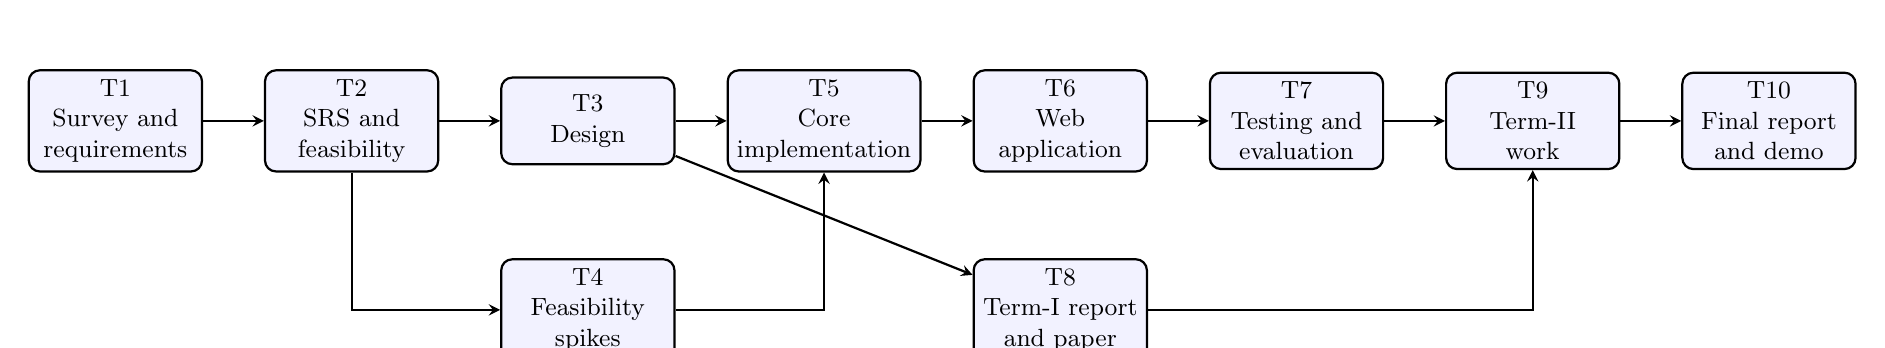
\begin{tikzpicture}[>=stealth, thick,
  task/.style={draw, rounded corners, minimum width=2.2cm, minimum height=1.1cm, align=center, font=\small, fill=blue!5}]
\node[task] (t1) at (0,0) {T1\\Survey and\\requirements};
\node[task] (t2) at (3,0) {T2\\SRS and\\feasibility};
\node[task] (t3) at (6,0) {T3\\Design};
\node[task] (t4) at (6,-2.4) {T4\\Feasibility\\spikes};
\node[task] (t5) at (9,0) {T5\\Core\\implementation};
\node[task] (t6) at (12,0) {T6\\Web\\application};
\node[task] (t7) at (15,0) {T7\\Testing and\\evaluation};
\node[task] (t8) at (12,-2.4) {T8\\Term-I report\\and paper};
\node[task] (t9) at (18,0) {T9\\Term-II\\work};
\node[task] (t10) at (21,0) {T10\\Final report\\and demo};
\draw[->] (t1) -- (t2);
\draw[->] (t2) -- (t3);
\draw[->] (t2) |- (t4);
\draw[->] (t3) -- (t5);
\draw[->] (t4) -| (t5);
\draw[->] (t5) -- (t6);
\draw[->] (t6) -- (t7);
\draw[->] (t3) -- (t8);
\draw[->] (t7) -- (t9);
\draw[->] (t8) -| (t9);
\draw[->] (t9) -- (t10);
\end{tikzpicture}}
\caption{Task network}
\label{fig:tasknet}
\end{figure}

\subsection{Timeline Chart}
The month-by-month timeline is in the planner in Annexure~\ref{app:plan}, drawn as a Gantt chart in Figure~\ref{fig:gantt}.


\section{Team Organization}
\label{sec:team}
The team consists of four students supervised by the internal guide. Work is divided by subsystem, and each subsystem has one owner and one reviewer.
\subsection{Team structure}
Table~\ref{tab:roles} lists the roles. The assignment of members to roles is to be completed by the team.

\begin{table}[!htbp]
\begin{center}
\def\arraystretch{1.4}
\begin{tabularx}{\textwidth}{| p{4.2cm} | X | p{2.8cm} |}
\hline
Role & Responsibilities & Member \\ \hline
Agent and verification & Planner, parallel search, synthesis prompt, claim verification, action store, evaluation harness & [to be filled] \\ \hline
Connectors and model router & Composio, MCP, Firecrawl and sample connectors; free-tier router, cooldowns and cache & [to be filled] \\ \hline
Memory service & FastAPI service, SQLite ledger, Oracle Agent Memory adapter, memory policy & [to be filled] \\ \hline
Web application and testing & Ask, Brief, Memory and Connections screens; event stream client; tests and documentation & [to be filled] \\ \hline
Internal guide & Review of design and progress, approval of milestones & Prof. [Guide Name] \\ \hline
\end{tabularx}
\end{center}
\caption{Team roles}
\label{tab:roles}
\end{table}

\subsection{Management reporting and communication}
We report to the guide in the project slots of the lab timetable, and progress is noted on the assessment sheet. Day to day, the Git repository is our record: every change lands as a commit with a message saying what and why, design decisions go into the docs folder, and nothing is merged until the tests and the evaluation have been run.


\chapter{Software requirement specification  }

\section{Introduction}
\subsection{Purpose and Scope of Document}
This chapter pins down what Cortex has to do and under which limits. It starts with who uses the system and why, moves on to the data it keeps and how a question flows through it, and ends with the non-functional requirements, design constraints and interfaces. We wrote it for ourselves, our guide and the examiners; the design in Chapter~\ref{ch:design} and the tests in Chapter~\ref{ch:testing} both trace back to it.

\subsection{Overview of responsibilities of Developer}
\begin{itemize}
\item Gather and document requirements; study the base paper and related literature.
\item Design the agent pipeline, the connector interface, the model router, the memory policy and the consent model.
\item Implement the web application, the packages and the memory service; keep secrets on the server only.
\item Write automated tests and an evaluation harness, run them before each change, and report results honestly.
\item Document installation, configuration and use; maintain the system as external APIs and free-tier limits change.
\end{itemize}

\section{Usage Scenario}
Below are the people and systems that interact with Cortex, followed by what each of them does with it.
 \subsection{User profiles}
\begin{itemize}
\item \textbf{End user} (primary actor): a developer, productivity-focused professional or undergraduate whose work is spread across Gmail, Google Calendar, Google Drive, Notion, Slack and GitHub. The user may be non-technical and never handles API keys or configuration files. The user asks questions, reads the Brief, approves or declines actions and manages memory.
\item \textbf{Operator} (deploys Cortex; may be the same person): places API keys in the server's environment file, optionally declares extra MCP servers in a configuration file, and starts the web server and the memory service.
\item \textbf{Connected applications} (secondary actor): Gmail, Google Calendar, Google Drive, Notion, Slack and GitHub through Composio; any MCP server; and the web through Firecrawl. They answer searches and, after approval, execute actions.
\item \textbf{Language model providers} (secondary actor): Groq, Google Gemini, Cerebras, OpenRouter and Puter, reached through OpenAI-compatible endpoints.
\item \textbf{Memory service} (secondary actor): the Python service that stores and searches memories, backed by SQLite or Oracle AI Database.
\end{itemize}

\subsection{Use-cases}
Table~\ref{tab:usecase} lists the eight use cases.

\begin{table}[!htbp]
\begin{center}
%\def\arraystretch{1.5}
\def\arraystretch{1.3}
\small
\begin{tabularx}{\textwidth}{| c | p{2.6cm} | X | p{2.3cm} | X |}
\hline
Sr No.	& Use Case	& Description	& Actors	& Assumptions \\
\hline
1& Ask a question & Cortex plans sub-questions, searches sources in parallel, streams a cited answer and verifies each claim & User, connected apps, model providers & At least one source connected and one provider key configured \\
\hline
2& Choose Fast or Deep mode & Fast: local single-step plan and one model call; Deep: model plan, empty-result retry and model re-check of doubtful claims & User & -- \\
\hline
3& Inspect trace and evidence & Open citations, cited sources, the plan, each tool call with its count and latency, and model usage & User & A run has started \\
\hline
4& Approve, edit or decline an action & Review the exact preview of a proposed action, optionally edit it, then approve (executes once) or decline & User, connected app & Proposal is pending, less than 30 minutes old, same user \\
\hline
5& Read the Daily Brief & Cited cards for what changed, what is at risk, conflicts and what is upcoming & User, connected apps, model providers & Sources connected \\
\hline
6& Manage memory & Teach a memory, pin, edit or forget it, and see why it was kept & User, memory service & Memory service running \\
\hline
7& Connect an app or choose a workspace & Start OAuth through Composio, or switch between the sample workspace and the user's own accounts & User, Composio & Composio key configured for own accounts \\
\hline
8& Add an MCP server & Declare a server, its search tool and its actions in the configuration file; no code change & Operator & Server reachable \\
\hline
\end{tabularx}
\end{center}
\caption{Use Cases}
\label{tab:usecase}
\end{table}


\subsection{Use Case View}
Figure~\ref{fig:usecase} draws the same use cases, with the user on the left and the supporting systems on the right.
\begin{center}
	\begin{figure}[!htbp]
		\centering
		\fbox{\resizebox{0.97\textwidth}{!}{%
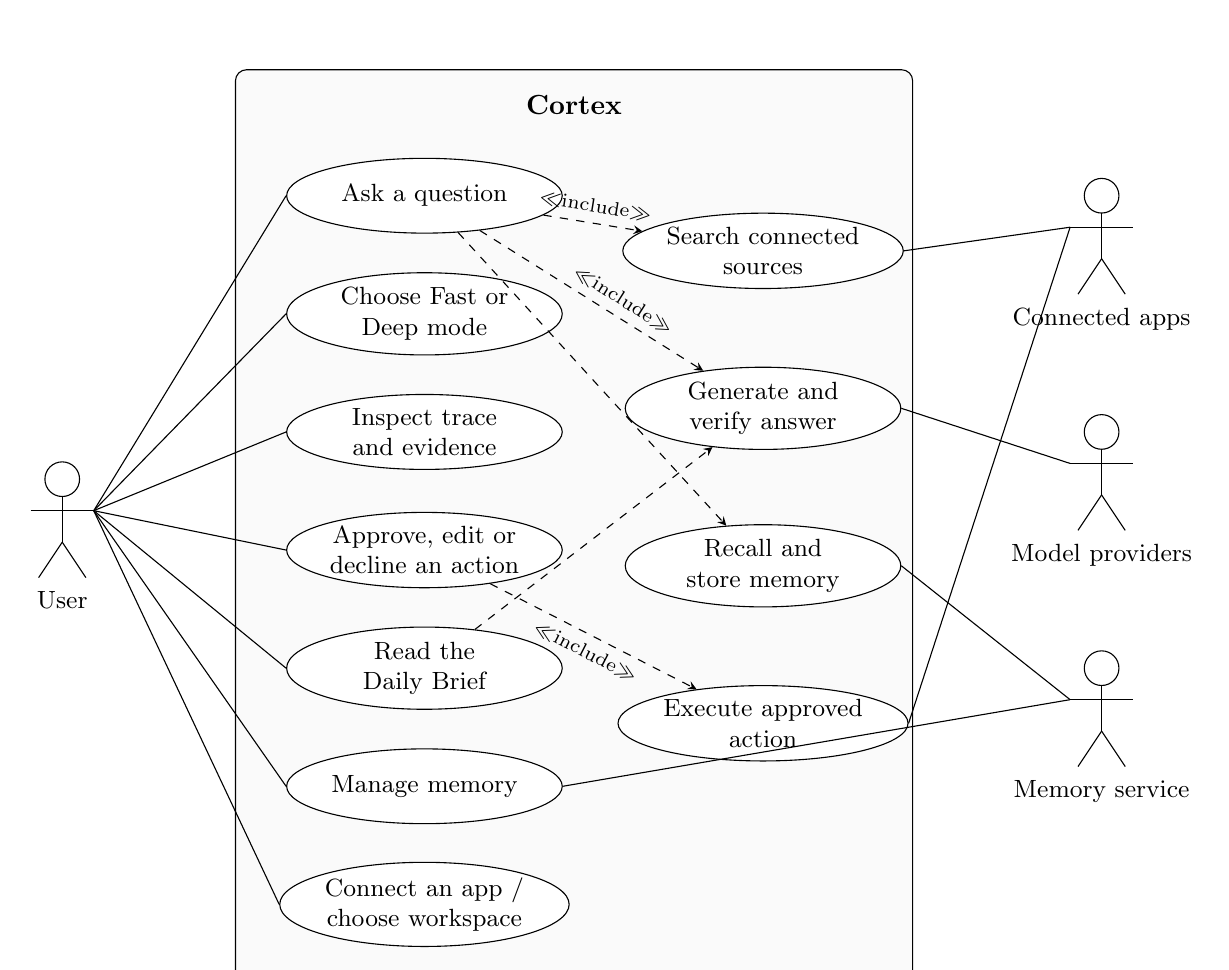
\begin{tikzpicture}[>=stealth,
  uc/.style={ellipse, draw, minimum width=3.5cm, minimum height=0.95cm, font=\small, align=center, inner sep=1pt, fill=white},
  inc/.style={->, dashed}]
\draw[rounded corners, fill=gray!4] (-3.4,0.9) rectangle (5.2,-10.7);
\node[font=\bfseries] at (0.9,0.45) {Cortex};
\node[uc] (u1) at (-1,-0.7) {Ask a question};
\node[uc] (u2) at (-1,-2.2) {Choose Fast or\\Deep mode};
\node[uc] (u3) at (-1,-3.7) {Inspect trace\\and evidence};
\node[uc] (u4) at (-1,-5.2) {Approve, edit or\\decline an action};
\node[uc] (u5) at (-1,-6.7) {Read the\\Daily Brief};
\node[uc] (u6) at (-1,-8.2) {Manage memory};
\node[uc] (u7) at (-1,-9.7) {Connect an app /\\choose workspace};
\node[uc] (u8) at (3.3,-1.4) {Search connected\\sources};
\node[uc] (u9) at (3.3,-3.4) {Generate and\\verify answer};
\node[uc] (u10) at (3.3,-5.4) {Recall and\\store memory};
\node[uc] (u11) at (3.3,-7.4) {Execute approved\\action};
\stickactor{-5.6}{-5.2}{User}
\stickactor{7.6}{-1.6}{Connected apps}
\stickactor{7.6}{-4.6}{Model providers}
\stickactor{7.6}{-7.6}{Memory service}
\foreach \uc in {u1,u2,u3,u4,u5,u6,u7} \draw (-5.2,-4.7) -- (\uc.west);
\draw[inc] (u1) -- node[above, sloped, font=\scriptsize] {$\ll$include$\gg$} (u8);
\draw[inc] (u1) -- node[above, sloped, font=\scriptsize, pos=0.6] {$\ll$include$\gg$} (u9);
\draw[inc] (u1) -- (u10);
\draw[inc] (u4) -- node[below, sloped, font=\scriptsize] {$\ll$include$\gg$} (u11);
\draw[inc] (u5) -- (u9);
\draw (u8.east) -- (7.2,-1.1);
\draw (u11.east) -- (7.2,-1.1);
\draw (u9.east) -- (7.2,-4.1);
\draw (u10.east) -- (7.2,-7.1);
\draw (u6.east) -- (7.2,-7.1);
\end{tikzpicture}}}
	  \caption{Use case diagram}
	  \label{fig:usecase}
	\end{figure}
\end{center}

\section{Data Model and Description}
\subsection{Data Description}
Cortex does not copy users' source data into a database: evidence exists only during a run (and in a 90~s search cache). The persistent data are the memories and the conversation messages kept by the memory service, and the response cache of the model router. The main data objects are:
\begin{itemize}
\item \textbf{Evidence}: one retrieved item, with a run-scoped identifier (\texttt{e1}, \texttt{e2}, \ldots), source, title, quote (a compact excerpt), and optional link, author, timestamp and sub-question identifier. Evidence is numbered in the prompt and cited as \texttt{[n]}.
\item \textbf{Plan} and \textbf{SubQuestion}: the run intent (\texttt{research}, \texttt{action} or \texttt{chat}), the rewritten question, an optional time window (since, until, label), and up to five sub-questions, each with its sources and a keyword query of at most 80 characters.
\item \textbf{Claim}: a sentence or list item of the answer, the identifiers of the evidence it cites, and its status (\texttt{supported}, \texttt{partial}, \texttt{unsupported}).
\item \textbf{Conflict}: a summary of a disagreement between sources and the identifiers of the evidence on each side.
\item \textbf{ActionProposal}: identifier, connector, action, title, a human-readable preview, arguments, risk (\texttt{low} or \texttt{high}), status (\texttt{pending}, \texttt{approved}, \texttt{rejected}, \texttt{executed}, \texttt{failed}) and result.
\item \textbf{MemoryItem}: identifier, user, content, kind (\texttt{priority}, \texttt{preference}, \texttt{fact}, \texttt{person}, \texttt{decision}), source, reason, salience in $[0,1]$, pinned flag, creation time, expiry time and the run that created it.
\item \textbf{SourceFailure}: the source, its display name, the reason (for example ``its connection expired; reconnect it'') and the impact on the answer.
\item \textbf{AgentEvent}: the unit of the output stream; one of sixteen typed events listed in Section~\ref{sec:io}.
\end{itemize}
\subsection{Data objects and Relationships}
Figure~\ref{fig:erd} draws these objects as an entity-relationship diagram. A run has one plan; a plan has up to five sub-questions; each sub-question yields evidence; a claim cites zero or more evidence items; a conflict refers to evidence from at least two sides; a run may produce action proposals and memories; and the messages of a run are appended to its conversation thread.

\begin{figure}[!htbp]
\centering
\resizebox{\textwidth}{!}{%
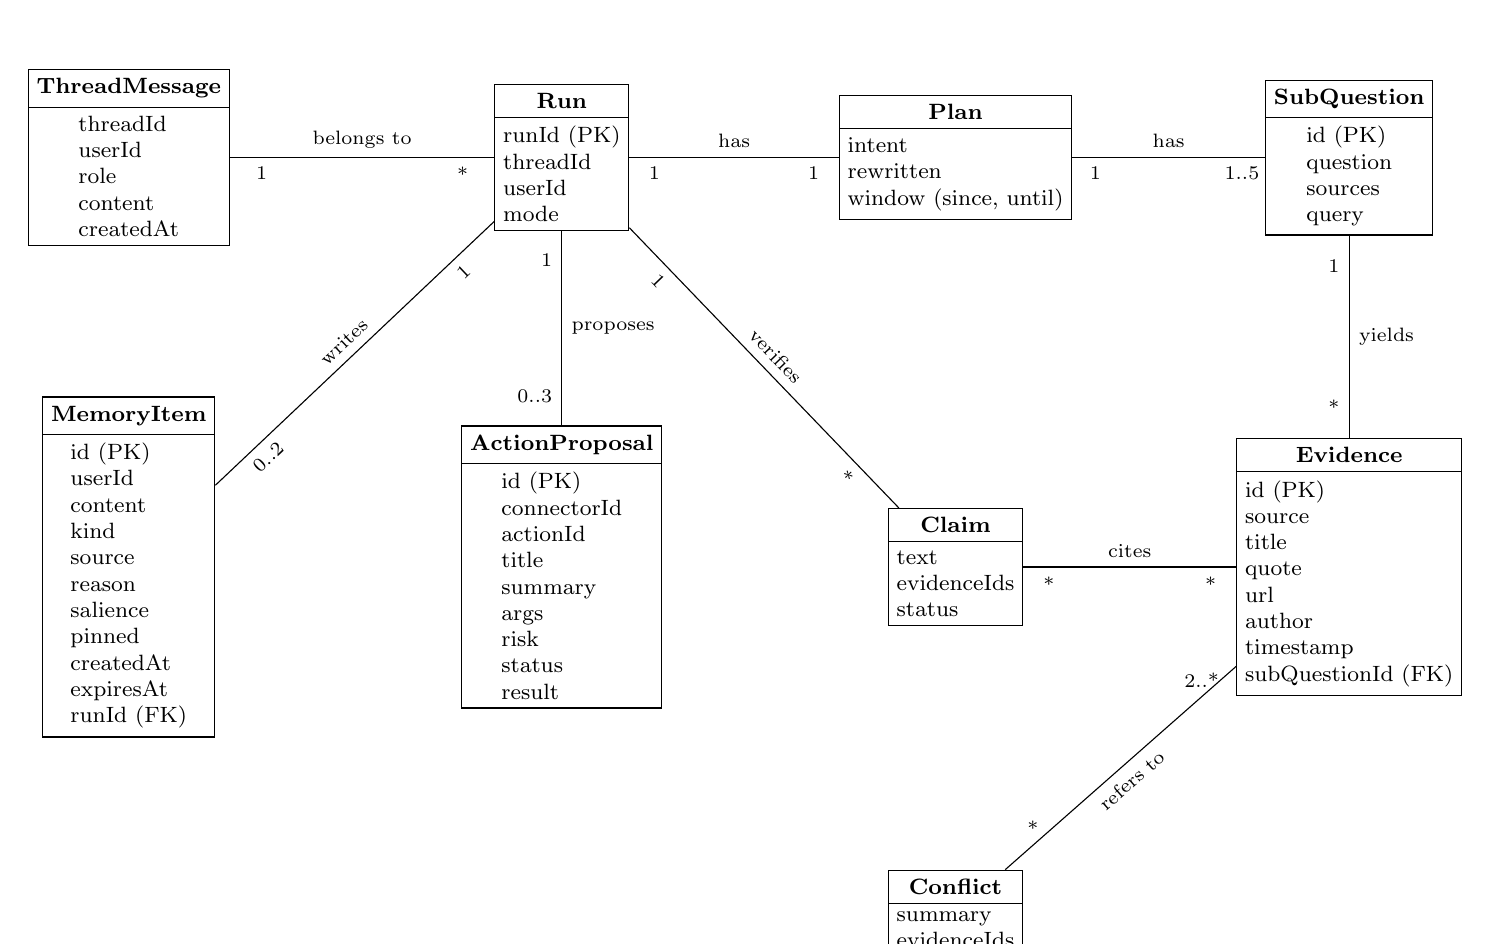
\begin{tikzpicture}[>=stealth,
  ent/.style={draw, rectangle split, rectangle split parts=2, align=left, font=\footnotesize, inner sep=3pt, fill=white, rectangle split part fill={blue!8,white}},
  rel/.style={font=\scriptsize}]
\node[ent] (thread) at (-5.5,0) {\textbf{ThreadMessage}\nodepart{second}threadId\\userId\\role\\content\\createdAt};
\node[ent] (run) at (0,0) {\textbf{Run}\nodepart{second}runId (PK)\\threadId\\userId\\mode};
\node[ent] (plan) at (5,0) {\textbf{Plan}\nodepart{second}intent\\rewritten\\window (since, until)};
\node[ent] (sq) at (10,0) {\textbf{SubQuestion}\nodepart{second}id (PK)\\question\\sources\\query};
\node[ent] (mem) at (-5.5,-5.2) {\textbf{MemoryItem}\nodepart{second}id (PK)\\userId\\content\\kind\\source\\reason\\salience\\pinned\\createdAt\\expiresAt\\runId (FK)};
\node[ent] (act) at (0,-5.2) {\textbf{ActionProposal}\nodepart{second}id (PK)\\connectorId\\actionId\\title\\summary\\args\\risk\\status\\result};
\node[ent] (claim) at (5,-5.2) {\textbf{Claim}\nodepart{second}text\\evidenceIds\\status};
\node[ent] (ev) at (10,-5.2) {\textbf{Evidence}\nodepart{second}id (PK)\\source\\title\\quote\\url\\author\\timestamp\\subQuestionId (FK)};
\node[ent] (conf) at (5,-9.6) {\textbf{Conflict}\nodepart{second}summary\\evidenceIds};
\draw (run) -- node[rel, above] {belongs to} node[rel, pos=0.12, below] {*} node[rel, pos=0.88, below] {1} (thread);
\draw (run) -- node[rel, above] {has} node[rel, pos=0.12, below] {1} node[rel, pos=0.88, below] {1} (plan);
\draw (plan) -- node[rel, above] {has} node[rel, pos=0.12, below] {1} node[rel, pos=0.88, below] {1..5} (sq);
\draw (sq) -- node[rel, right] {yields} node[rel, pos=0.15, left] {1} node[rel, pos=0.85, left] {*} (ev);
\draw (claim) -- node[rel, above] {cites} node[rel, pos=0.12, below] {*} node[rel, pos=0.88, below] {*} (ev);
\draw (conf) -- node[rel, below, sloped] {refers to} node[rel, pos=0.12, above] {*} node[rel, pos=0.85, above] {2..*} (ev);
\draw (run) -- node[rel, right] {proposes} node[rel, pos=0.15, left] {1} node[rel, pos=0.85, left] {0..3} (act);
\draw (run) -- node[rel, above, sloped] {writes} node[rel, pos=0.15, below, sloped] {1} node[rel, pos=0.85, below, sloped] {0..2} (mem);
\draw (run) -- node[rel, above, sloped] {verifies} node[rel, pos=0.15, below, sloped] {1} node[rel, pos=0.85, below, sloped] {*} (claim);
\end{tikzpicture}}
\caption{Data objects and relationships (ERD form)}
\label{fig:erd}
\end{figure}



\section{Functional Model and Description}
This section walks through what Cortex does with a question, as data flows; the classes behind it are in Chapter~\ref{ch:design}. A run uses nine functions: (1) check which sources are available; (2) recall memories; (3) plan; (4) search in parallel and rank evidence; (5) synthesize a streamed, cited answer; (6) verify claims and compute groundedness; (7) validate and store action proposals; (8) remember salient facts; and (9) execute an approved action. The Daily Brief reuses functions (1), (2), (4) and a single synthesis call.
\subsection{Data Flow Diagram}
\subsubsection{Level 0 Data Flow Diagram}
Figure~\ref{fig:dfd0} shows Cortex as a single process with its external entities.

\begin{figure}[!htbp]
\centering
\resizebox{\textwidth}{!}{%
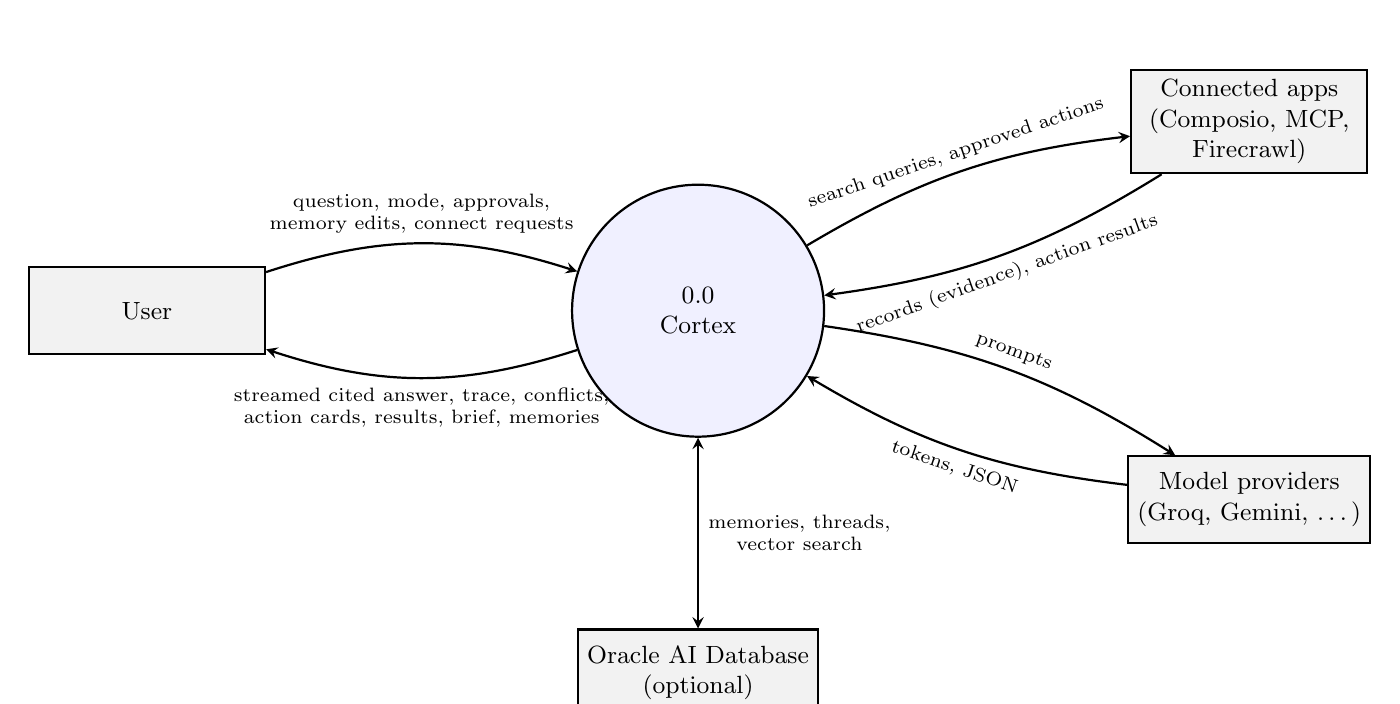
\begin{tikzpicture}[>=stealth, thick,
  ext/.style={draw, rectangle, minimum width=3cm, minimum height=1.1cm, align=center, font=\small, fill=gray!10},
  proc/.style={draw, circle, minimum size=3.2cm, align=center, font=\small, fill=blue!6},
  lab/.style={font=\scriptsize, align=center}]
\node[ext] (user) at (-7,0) {User};
\node[proc] (p0) at (0,0) {0.0\\Cortex};
\node[ext] (apps) at (7,2.4) {Connected apps\\(Composio, MCP,\\Firecrawl)};
\node[ext] (llm) at (7,-2.4) {Model providers\\(Groq, Gemini, \ldots)};
\node[ext] (ora) at (0,-4.6) {Oracle AI Database\\(optional)};
\draw[->] (user) to[bend left=18] node[lab, above] {question, mode, approvals,\\memory edits, connect requests} (p0);
\draw[->] (p0) to[bend left=18] node[lab, below] {streamed cited answer, trace, conflicts,\\action cards, results, brief, memories} (user);
\draw[->] (p0) to[bend left=12] node[lab, above, sloped] {search queries, approved actions} (apps);
\draw[->] (apps) to[bend left=12] node[lab, below, sloped] {records (evidence), action results} (p0);
\draw[->] (p0) to[bend left=12] node[lab, above, sloped] {prompts} (llm);
\draw[->] (llm) to[bend left=12] node[lab, below, sloped] {tokens, JSON} (p0);
\draw[<->] (p0) -- node[lab, right] {memories, threads,\\vector search} (ora);
\end{tikzpicture}}
\caption{Level 0 data flow diagram}
\label{fig:dfd0}
\end{figure}

\subsubsection{Level 1 Data Flow Diagram}
Figure~\ref{fig:dfd1} decomposes the process into its nine sub-processes. External entities and data stores marked with an asterisk are repeated to keep lines short. The response cache and the search cache are omitted for clarity.

\begin{figure}[!htbp]
\centering
\resizebox{!}{0.82\textheight}{%
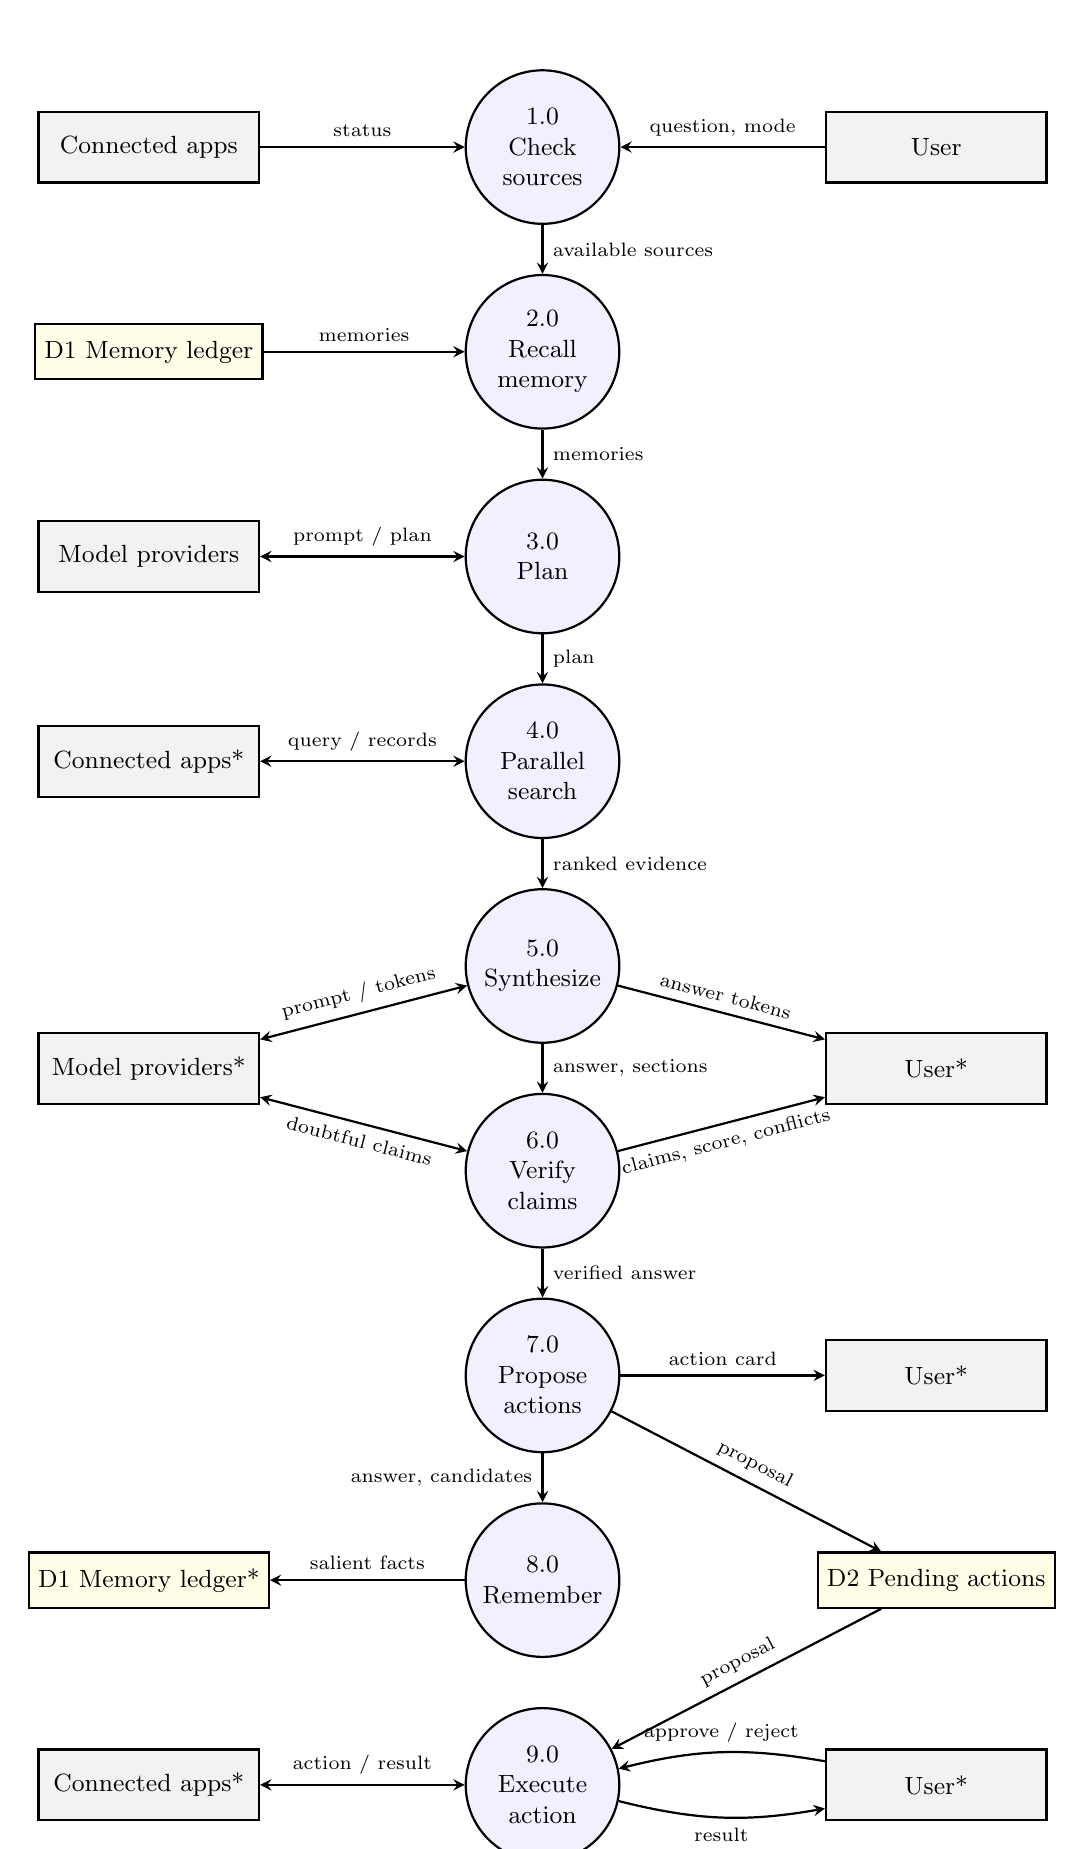
\begin{tikzpicture}[>=stealth, thick,
  ext/.style={draw, rectangle, minimum width=2.8cm, minimum height=0.9cm, align=center, font=\small, fill=gray!10},
  store/.style={draw, rectangle, minimum width=2.8cm, minimum height=0.7cm, align=center, font=\small, fill=yellow!10},
  proc/.style={draw, circle, minimum size=1.95cm, align=center, font=\small, fill=blue!6, inner sep=1pt},
  lab/.style={font=\scriptsize, align=center}]
\node[proc] (p1) at (5,0) {1.0\\Check\\sources};
\node[proc] (p2) at (5,-2.6) {2.0\\Recall\\memory};
\node[proc] (p3) at (5,-5.2) {3.0\\Plan};
\node[proc] (p4) at (5,-7.8) {4.0\\Parallel\\search};
\node[proc] (p5) at (5,-10.4) {5.0\\Synthesize};
\node[proc] (p6) at (5,-13) {6.0\\Verify\\claims};
\node[proc] (p7) at (5,-15.6) {7.0\\Propose\\actions};
\node[proc] (p8) at (5,-18.2) {8.0\\Remember};
\node[proc] (p9) at (5,-20.8) {9.0\\Execute\\action};
\node[ext] (apps) at (0,0) {Connected apps};
\node[store] (d1) at (0,-2.6) {D1 Memory ledger};
\node[ext] (llm1) at (0,-5.2) {Model providers};
\node[ext] (apps2) at (0,-7.8) {Connected apps*};
\node[ext] (llm2) at (0,-11.7) {Model providers*};
\node[store] (d1b) at (0,-18.2) {D1 Memory ledger*};
\node[ext] (apps3) at (0,-20.8) {Connected apps*};
\node[ext] (user) at (10,0) {User};
\node[ext] (user2) at (10,-11.7) {User*};
\node[ext] (user3) at (10,-15.6) {User*};
\node[store] (d2) at (10,-18.2) {D2 Pending actions};
\node[ext] (user4) at (10,-20.8) {User*};
\draw[->] (user) -- node[lab, above] {question, mode} (p1);
\draw[->] (apps) -- node[lab, above] {status} (p1);
\draw[->] (d1) -- node[lab, above] {memories} (p2);
\draw[<->] (llm1) -- node[lab, above] {prompt / plan} (p3);
\draw[<->] (apps2) -- node[lab, above] {query / records} (p4);
\draw[<->] (llm2) -- node[lab, above, sloped] {prompt / tokens} (p5);
\draw[<->] (llm2) -- node[lab, below, sloped] {doubtful claims} (p6);
\draw[->] (p8) -- node[lab, above] {salient facts} (d1b);
\draw[<->] (p9) -- node[lab, above] {action / result} (apps3);
\draw[->] (p1) -- node[lab, right] {available sources} (p2);
\draw[->] (p2) -- node[lab, right] {memories} (p3);
\draw[->] (p3) -- node[lab, right] {plan} (p4);
\draw[->] (p4) -- node[lab, right] {ranked evidence} (p5);
\draw[->] (p5) -- node[lab, right] {answer, sections} (p6);
\draw[->] (p6) -- node[lab, right] {verified answer} (p7);
\draw[->] (p7) -- node[lab, left] {answer, candidates} (p8);
\draw[->] (p5) -- node[lab, above, sloped] {answer tokens} (user2);
\draw[->] (p6) -- node[lab, below, sloped] {claims, score, conflicts} (user2);
\draw[->] (p7) -- node[lab, above] {action card} (user3);
\draw[->] (p7) -- node[lab, above, sloped] {proposal} (d2);
\draw[->] (d2) -- node[lab, above, sloped] {proposal} (p9);
\draw[->] (user4) to[bend right=12] node[lab, above] {approve / reject} (p9);
\draw[->] (p9) to[bend right=12] node[lab, below] {result} (user4);
\end{tikzpicture}}
\caption{Level 1 data flow diagram}
\label{fig:dfd1}
\end{figure}





\subsection{Activity Diagram:}
\begin{itemize}
	\item	Figure~\ref{fig:activity} follows one run from question to stored memory. The diamonds are the four branch points (Fast mode, small talk, no evidence, action requested), and the bars mark where the searches fork and join.
\end{itemize}

\begin{figure}[!htbp]
\centering
\resizebox{!}{0.85\textheight}{%
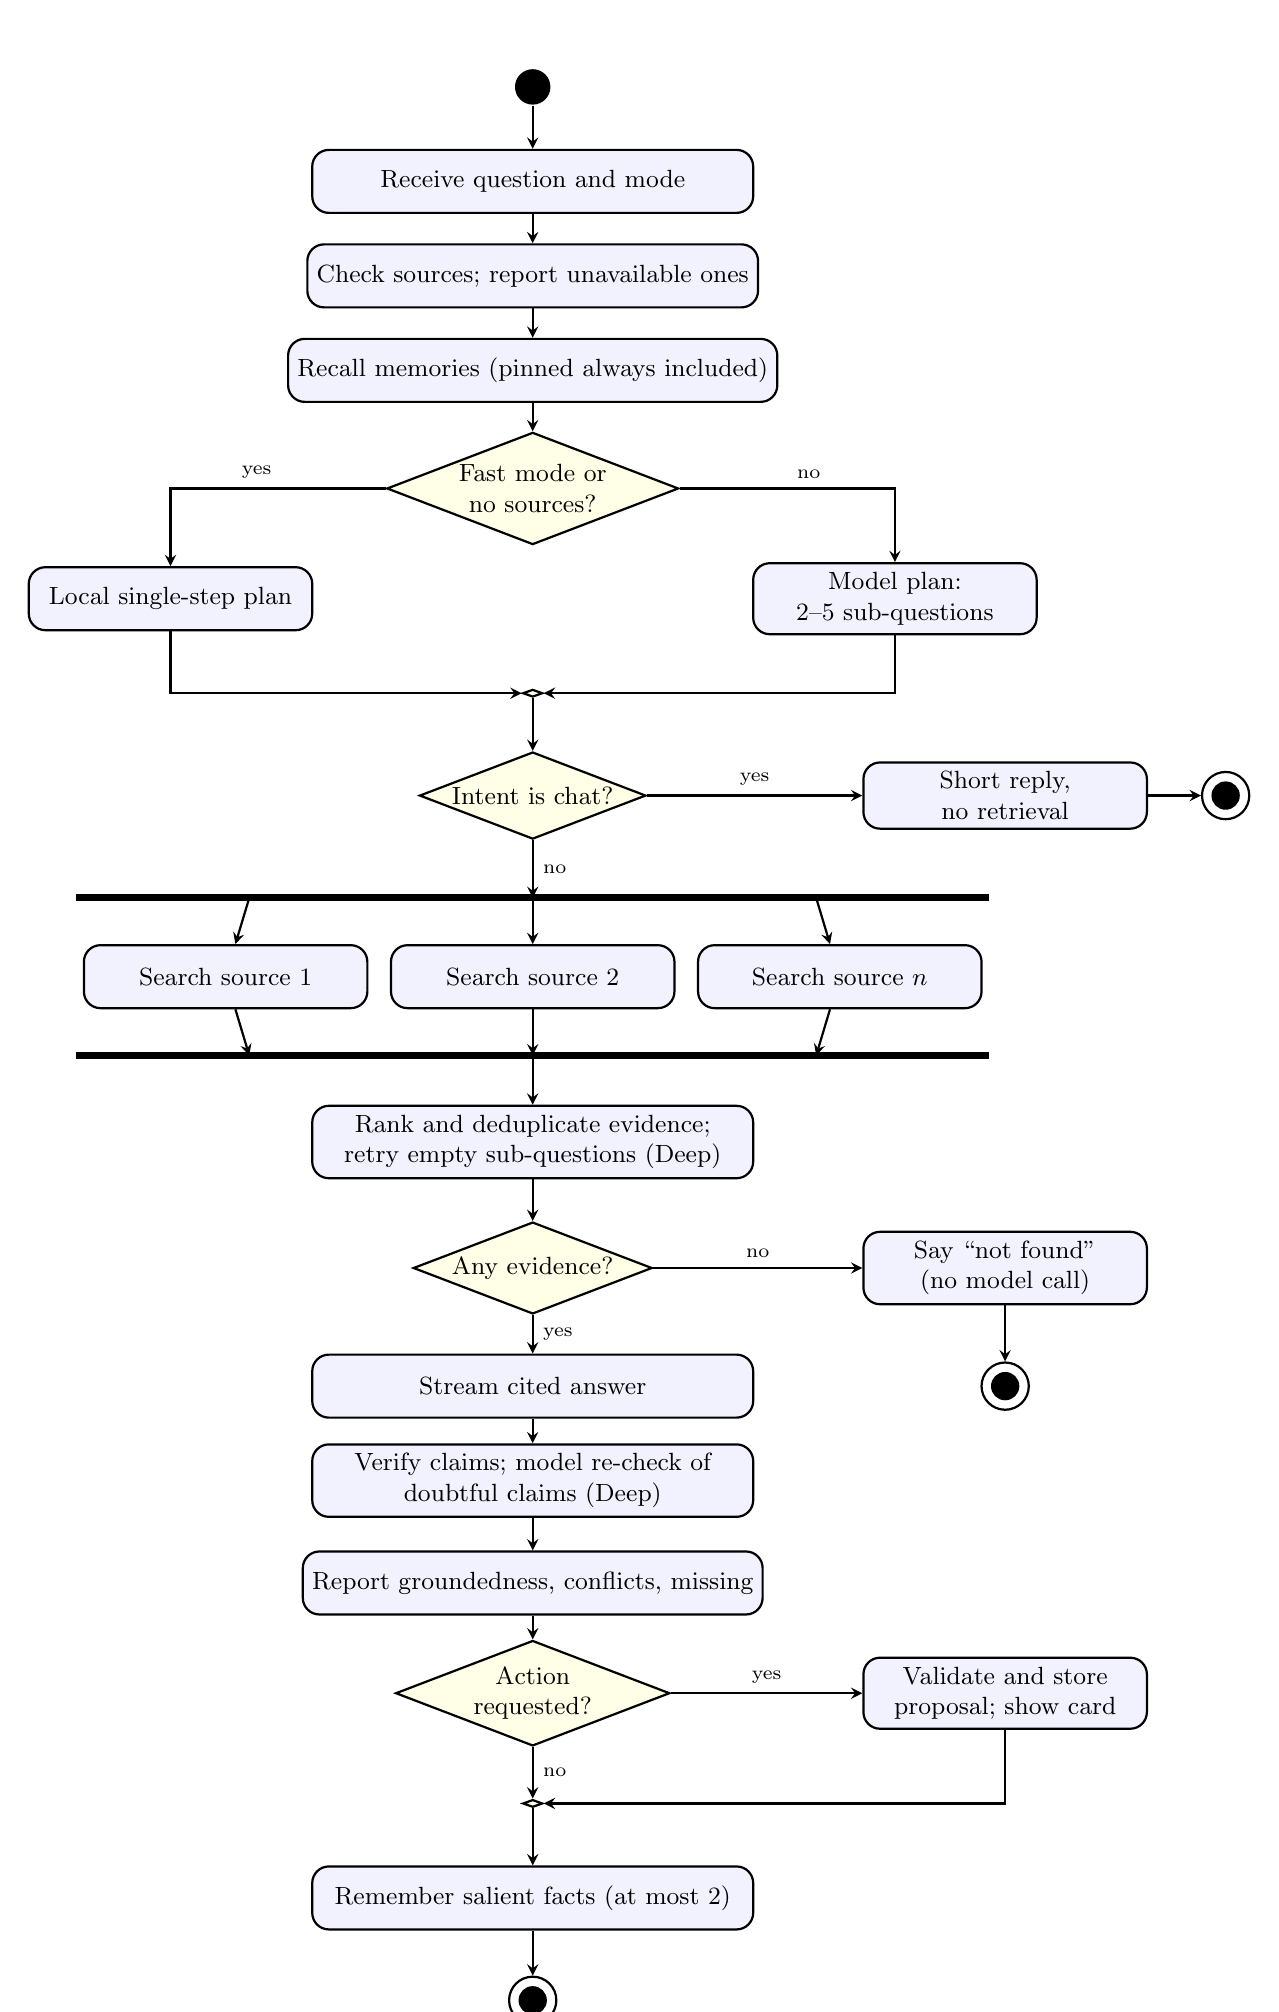
\begin{tikzpicture}[>=stealth, thick,
  act/.style={draw, rounded corners=6pt, minimum width=5.6cm, minimum height=0.8cm, align=center, font=\small, fill=blue!5},
  side/.style={draw, rounded corners=6pt, minimum width=3.6cm, minimum height=0.8cm, align=center, font=\small, fill=blue!5},
  dec/.style={draw, diamond, aspect=2.6, align=center, font=\small, inner sep=1pt, fill=yellow!10},
  lab/.style={font=\scriptsize}]
\node[circle, fill=black, minimum size=0.45cm] (start) at (0,0) {};
\node[act] (a1) at (0,-1.2) {Receive question and mode};
\node[act] (a2) at (0,-2.4) {Check sources; report unavailable ones};
\node[act] (a3) at (0,-3.6) {Recall memories (pinned always included)};
\node[dec] (d1) at (0,-5.1) {Fast mode or\\no sources?};
\node[side] (a4) at (-4.6,-6.5) {Local single-step plan};
\node[side] (a5) at (4.6,-6.5) {Model plan:\\2--5 sub-questions};
\node[dec] (m1) at (0,-7.7) {};
\node[dec] (d2) at (0,-9.0) {Intent is chat?};
\node[side] (a6) at (6,-9.0) {Short reply,\\no retrieval};
\draw[line width=2.5pt] (-5.8,-10.3) -- (5.8,-10.3);
\node[side] (s1) at (-3.9,-11.3) {Search source 1};
\node[side] (s2) at (0,-11.3) {Search source 2};
\node[side] (s3) at (3.9,-11.3) {Search source $n$};
\draw[line width=2.5pt] (-5.8,-12.3) -- (5.8,-12.3);
\node[act] (a7) at (0,-13.4) {Rank and deduplicate evidence;\\retry empty sub-questions (Deep)};
\node[dec] (d3) at (0,-15.0) {Any evidence?};
\node[side] (a8) at (6,-15.0) {Say ``not found''\\(no model call)};
\node[act] (a9) at (0,-16.5) {Stream cited answer};
\node[act] (a10) at (0,-17.7) {Verify claims; model re-check of\\doubtful claims (Deep)};
\node[act] (a11) at (0,-19.0) {Report groundedness, conflicts, missing};
\node[dec] (d4) at (0,-20.4) {Action\\requested?};
\node[side] (a12) at (6,-20.4) {Validate and store\\proposal; show card};
\node[dec] (m2) at (0,-21.8) {};
\node[act] (a13) at (0,-23.0) {Remember salient facts (at most 2)};
\node[circle, draw, minimum size=0.6cm] (end) at (0,-24.3) {};
\node[circle, fill=black, minimum size=0.36cm] at (0,-24.3) {};
\node[circle, draw, minimum size=0.6cm] (end2) at (8.8,-9.0) {};
\node[circle, fill=black, minimum size=0.36cm] at (8.8,-9.0) {};
\node[circle, draw, minimum size=0.6cm] (end3) at (6,-16.5) {};
\node[circle, fill=black, minimum size=0.36cm] at (6,-16.5) {};
\draw[->] (start) -- (a1);
\draw[->] (a1) -- (a2);
\draw[->] (a2) -- (a3);
\draw[->] (a3) -- (d1);
\draw[->] (d1) -| node[lab, above, pos=0.3] {yes} (a4);
\draw[->] (d1) -| node[lab, above, pos=0.3] {no} (a5);
\draw[->] (a4) |- (m1);
\draw[->] (a5) |- (m1);
\draw[->] (m1) -- (d2);
\draw[->] (d2) -- node[lab, above] {yes} (a6);
\draw[->] (a6) -- (end2);
\draw[->] (d2) -- node[lab, right] {no} (0,-10.3);
\draw[->] (-3.6,-10.3) -- (s1);
\draw[->] (0,-10.3) -- (s2);
\draw[->] (3.6,-10.3) -- (s3);
\draw[->] (s1) -- (-3.6,-12.3);
\draw[->] (s2) -- (0,-12.3);
\draw[->] (s3) -- (3.6,-12.3);
\draw[->] (0,-12.3) -- (a7);
\draw[->] (a7) -- (d3);
\draw[->] (d3) -- node[lab, above] {no} (a8);
\draw[->] (a8) -- (end3);
\draw[->] (d3) -- node[lab, right] {yes} (a9);
\draw[->] (a9) -- (a10);
\draw[->] (a10) -- (a11);
\draw[->] (a11) -- (d4);
\draw[->] (d4) -- node[lab, above] {yes} (a12);
\draw[->] (a12) |- (m2);
\draw[->] (d4) -- node[lab, right] {no} (m2);
\draw[->] (m2) -- (a13);
\draw[->] (a13) -- (end);
\end{tikzpicture}}
\caption{Activity diagram of one agent run}
\label{fig:activity}
\end{figure}

\subsection{Non Functional Requirements:}
\begin{itemize}
	\item	\textbf{Interface Requirements:} a responsive web interface usable on a laptop and on a phone; answers streamed as they are written; the reasoning trace available but collapsed by default; a JSON/HTTP and server-sent event interface between browser and server; an HTTP/JSON interface to the memory service; OpenAI-compatible chat-completion interfaces to model providers; MCP (streamable HTTP or standard input/output) and the Composio SDK to connected apps.
	\item	\textbf{Performance Requirements:} the answer should begin streaming within a few seconds; searches run concurrently; each connector call times out after 12~s (one retry), each connector status check after 6~s, each model request after 25~s and each memory request after 5~s; a whole run is stopped after 90~s. The preliminary evaluation measured a median end-to-end time of 3.7~s and a 90th percentile of 7.1~s in Deep mode.
    \item	\textbf{Software quality attributes:}
    \begin{itemize}
    \item \emph{Availability} (related to reliability): provider failover with cooldowns; a failed source is reported and skipped; the run continues without memory if the memory service is down; the memory service continues on SQLite if Oracle is down.
    \item \emph{Modifiability} (portability, reusability, scalability): a new source is one class implementing the connector interface, or one entry in the MCP configuration file; Composio tool names are data; model identifiers are environment variables; the agent, router, connectors and shared types are separate packages; the code runs on Windows, Linux and macOS. Horizontal scaling is limited because pending actions and caches are held in the memory of one server process.
    \item \emph{Performance}: bounded calls per run; caching of responses (6~h) and searches (90~s).
    \item \emph{Security}: actions only through the approval endpoint, once, for the proposing user; OAuth tokens held by Composio, never sent to the browser; an HTTP-only, same-site cookie for the anonymous identifier; memories of the sample workspace kept separate from real ones.
    \item \emph{Testability}: all external dependencies are passed in through one dependency object, so tests replace them with stubs; 18 automated tests; an evaluation harness.
    \item \emph{Usability}: plain-language failure messages; claims visually marked by verification state; one-click connection; no settings pages or tokens for the end user.
    \end{itemize}
\end{itemize}

\subsection{State Diagram:}
  State Transition Diagram\\
Fig.\ref{fig:state-dig} tracks a single action proposal. It is born when the model drafts an action and the store accepts it, and it ends in one of five places: discarded, rejected, expired, executed or failed (double borders). Each arrow is labelled with the event that moves it. There is no arrow from \emph{Pending} straight to \emph{Executed}; the only way through is an explicit approval.

\begin{center}
	\begin{figure}[!htbp]
		\centering
		\fbox{\resizebox{0.95\textwidth}{!}{%
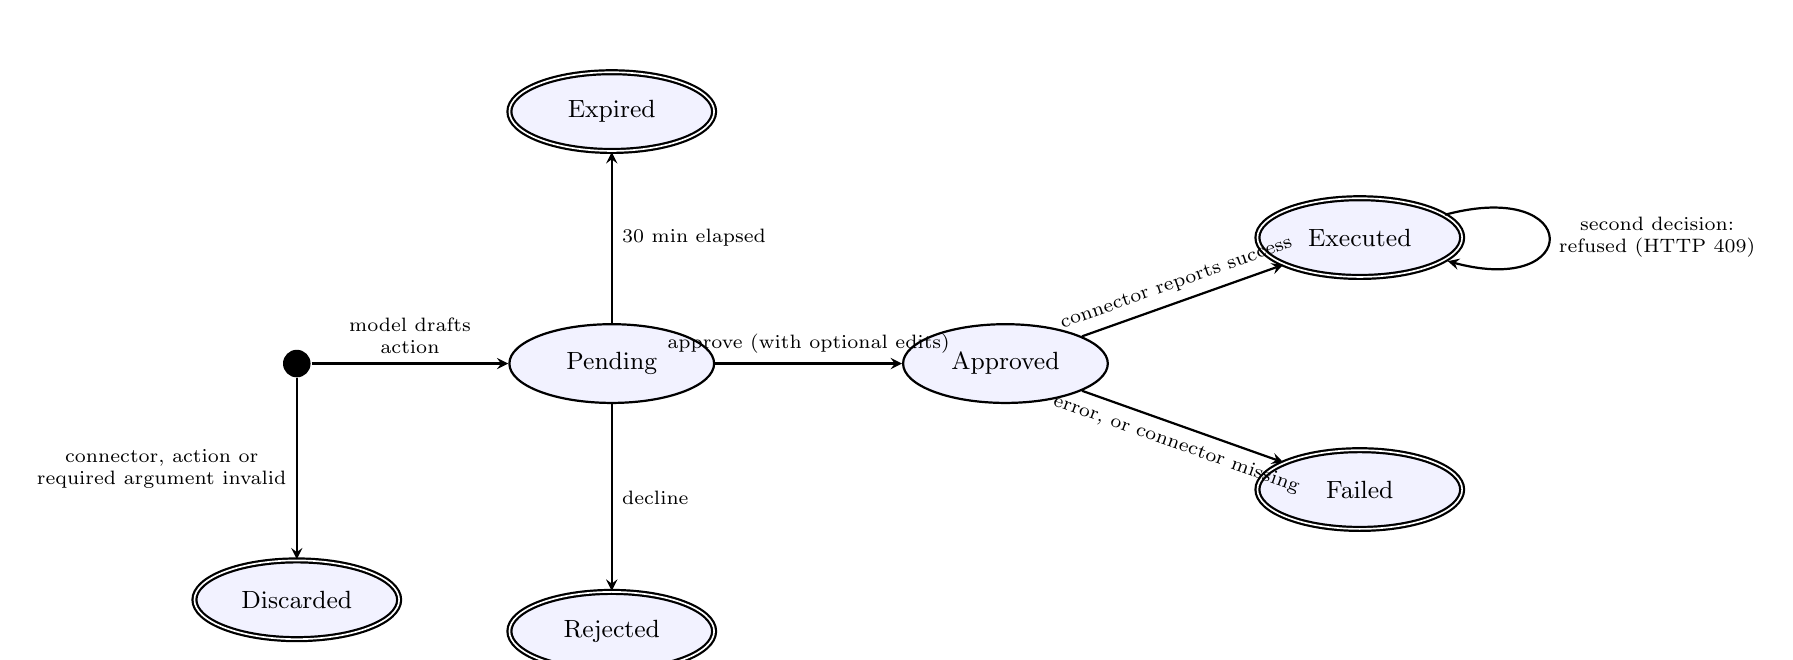
\begin{tikzpicture}[->, >=stealth, thick, auto,
  st/.style={draw, ellipse, minimum width=2.6cm, minimum height=1cm, align=center, font=\small, fill=blue!5},
  fin/.style={st, double},
  lab/.style={font=\scriptsize, align=center}]
\node[circle, fill=black, minimum size=0.35cm] (init) at (0,0) {};
\node[fin] (disc) at (0,-3) {Discarded};
\node[st] (pend) at (4,0) {Pending};
\node[fin] (rej) at (4,-3.4) {Rejected};
\node[fin] (exp) at (4,3.2) {Expired};
\node[st] (appr) at (9,0) {Approved};
\node[fin] (exec) at (13.5,1.6) {Executed};
\node[fin] (fail) at (13.5,-1.6) {Failed};
\draw (init) -- node[lab, above] {model drafts\\action} (pend);
\draw (init) -- node[lab, left] {connector, action or\\required argument invalid} (disc);
\draw (pend) -- node[lab, right] {decline} (rej);
\draw (pend) -- node[lab, right] {30 min elapsed} (exp);
\draw (pend) -- node[lab, above] {approve (with optional edits)} (appr);
\draw (appr) -- node[lab, above, sloped] {connector reports success} (exec);
\draw (appr) -- node[lab, below, sloped] {error, or connector missing} (fail);
\draw (exec) edge[loop right] node[lab, right] {second decision:\\refused (HTTP 409)} (exec);
\end{tikzpicture}}}
	  \caption{State transition diagram}
	  \label{fig:state-dig}
	\end{figure}
\end{center}

 \subsection{Design Constraints}
\begin{itemize}
\item Only free-tier services may be used, which bounds model calls per run and requires failover and caching.
\item Oracle Agent Memory has only a Python SDK, so memory is a separate Python service.
\item Streaming requires a server runtime that keeps the HTTP response open (server-sent events in a Next.js route handler).
\item Pending actions are held in the server's memory with a 30-minute lifetime; a restart discards them, which is safe (nothing executes) but requires asking again.
\item Evidence quotes are compacted to a few hundred characters to keep prompts small.
\item Node.js 24 or later and Python 3.11 are required.
\end{itemize}
 \subsection{Software Interface Description}
Table~\ref{tab:interfaces} lists every endpoint Cortex exposes or calls. People use the web screens shown in Chapter~\ref{ch:results}.

\begin{table}[!htbp]
\begin{center}
\def\arraystretch{1.25}
\small
\begin{tabularx}{\textwidth}{| p{5.2cm} | X |}
\hline
Interface & Purpose \\ \hline
\multicolumn{2}{|l|}{\textbf{Web server (browser to server)}} \\ \hline
\texttt{POST /api/ask} & Run the agent; response is a server-sent event stream \\ \hline
\texttt{POST /api/actions/\{id\}} & Approve or reject one proposal; the only execution path \\ \hline
\texttt{GET /api/brief} & Daily Brief \\ \hline
\texttt{GET, POST /api/memory} & List memories; teach a memory \\ \hline
\texttt{PATCH, DELETE /api/memory/\{id\}} & Pin or edit; forget \\ \hline
\texttt{GET, PUT /api/connections} & Connection status; choose workspace \\ \hline
\texttt{POST /api/connections/\{id\}} & Start OAuth for one app \\ \hline
\multicolumn{2}{|l|}{\textbf{Memory service (server to service, HTTP/JSON)}} \\ \hline
\texttt{GET /health} & Status and active backend (\texttt{oracle} or \texttt{sqlite}) \\ \hline
\texttt{GET, POST /memories} & List; add (near-duplicates reinforce an existing memory) \\ \hline
\texttt{PATCH, DELETE /memories/\{id\}} & Edit or pin; forget \\ \hline
\texttt{POST /search} & Recall: pinned memories plus ranked matches \\ \hline
\texttt{POST /threads/\{id\}/messages} & Append conversation turns \\ \hline
\texttt{GET /threads/\{id\}/context} & Thread summary (Oracle) and recent messages \\ \hline
\multicolumn{2}{|l|}{\textbf{External}} \\ \hline
OpenAI-compatible chat completions & Groq, Gemini, Cerebras, OpenRouter, Puter \\ \hline
Composio SDK / hosted MCP & Gmail, Calendar, Drive, Notion, Slack, GitHub tools and OAuth \\ \hline
MCP (HTTP or stdio) & Any server declared in \texttt{mcp.config.json} \\ \hline
Firecrawl API & Web search and page scraping \\ \hline
LangSmith API & Optional traces of runs, model calls and searches \\ \hline
\end{tabularx}
\end{center}
\caption{Software interfaces}
\label{tab:interfaces}
\end{table}



\chapter{Detailed Design Document using Appendix A and B}
\label{ch:design}
 \section{Introduction}
This chapter explains how Cortex is built to answer questions over scattered, live work data with cited and checked answers, and to act only with consent. It covers the architecture, then the data, then the components. The design follows four principles taken from the project's product definition: show the evidence and not only the answer; never act without consent; say ``I don't know'' before guessing; and keep every loop bounded.
\section{Architectural Design}
	Cortex is a layered system (Figure~\ref{fig:arch-dig}). The \textbf{browser client} (React) renders the Ask, Brief, Memory and Connections screens and consumes the event stream. The \textbf{web server} (Next.js route handlers) authenticates the browser by an anonymous cookie, builds the dependencies for the selected workspace and exposes the API. The \textbf{agent package} contains the orchestrator, the prompts, the verifier, the action store, the brief and the tracing wrapper. It depends on three subsystems: the \textbf{model router} package, the \textbf{connector} package and the \textbf{memory service}. A \textbf{shared} package holds the types used by both server and client. The orchestrator is written by hand rather than with a graph framework, so that every branch is explicit, every loop is bounded and the number of model calls is predictable.

\textbf{Package view.} \texttt{apps/web} depends on \texttt{packages/agent}, \texttt{packages/connectors}, \texttt{packages/llm} and \texttt{packages/shared}; \texttt{packages/agent} depends on the other three packages; \texttt{packages/connectors} uses the cache of \texttt{packages/llm}; \texttt{services/memory} is independent and is reached over HTTP.

\textbf{Deployment view.} During development and evaluation, two processes run on one machine: the Next.js server on port 3000 and the memory service (Uvicorn) on port 8000. The optional Oracle AI Database Free runs in a Docker container on port 1521. All other services are remote APIs. Deployment to a hosted environment is planned for Term II.

  \begin{center}
	\begin{figure}[!htbp]
		\centering
		\fbox{\resizebox{0.97\textwidth}{!}{%
\begin{tikzpicture}[>=stealth, thick,
  layer/.style={draw, rounded corners, fill=gray!6},
  box/.style={draw, rounded corners=3pt, align=center, font=\small, fill=white, minimum height=0.9cm},
  step/.style={draw, rounded corners=3pt, align=center, font=\scriptsize, fill=blue!8, minimum height=0.8cm, minimum width=1.6cm},
  ext/.style={draw, align=center, font=\small, fill=yellow!10, minimum height=1cm},
  ttl/.style={font=\small\bfseries, anchor=west}]
% browser
\draw[layer] (0,1) rectangle (17,-1.3);
\node[ttl] at (0.1,0.7) {Browser (React client)};
\node[box, minimum width=2.9cm] at (2,-0.5) {Ask + live trace};
\node[box, minimum width=2.9cm] at (5.3,-0.5) {Brief};
\node[box, minimum width=2.9cm] at (8.6,-0.5) {Memory inspector};
\node[box, minimum width=2.9cm] at (11.9,-0.5) {Connections};
\node[box, minimum width=2.6cm] at (15.2,-0.5) {useAgent\\(SSE client)};
\draw[<->] (8.5,-1.3) -- node[right, font=\small] {HTTPS: JSON requests, server-sent events} (8.5,-2.1);
% server
\draw[layer] (0,-2.1) rectangle (17,-4.3);
\node[ttl] at (0.1,-2.4) {Next.js server (apps/web)};
\node[box, minimum width=2.4cm, font=\scriptsize] at (1.6,-3.5) {/api/ask\\(SSE)};
\node[box, minimum width=2.4cm, font=\scriptsize] at (4.3,-3.5) {/api/actions/[id]\\(only executor)};
\node[box, minimum width=2.4cm, font=\scriptsize] at (7.0,-3.5) {/api/brief};
\node[box, minimum width=2.4cm, font=\scriptsize] at (9.7,-3.5) {/api/memory};
\node[box, minimum width=2.4cm, font=\scriptsize] at (12.4,-3.5) {/api/connections};
\node[box, minimum width=2.4cm, font=\scriptsize] at (15.2,-3.5) {proxy\\(anonymous id)};
\draw[->] (8.5,-4.3) -- (8.5,-5.0);
% agent
\draw[layer] (0,-5.0) rectangle (17,-8.6);
\node[ttl] at (0.1,-5.3) {packages/agent};
\node[step] (s1) at (1.2,-6.3) {understand};
\node[step] (s2) at (3.3,-6.3) {recall};
\node[step] (s3) at (5.4,-6.3) {plan};
\node[step] (s4) at (7.5,-6.3) {search\\(parallel)};
\node[step] (s5) at (9.6,-6.3) {synthesize\\(stream)};
\node[step] (s6) at (11.7,-6.3) {verify};
\node[step] (s7) at (13.8,-6.3) {propose\\actions};
\node[step] (s8) at (15.9,-6.3) {remember};
\foreach \sa/\sb in {s1/s2,s2/s3,s3/s4,s4/s5,s5/s6,s6/s7,s7/s8} \draw[->] (\sa) -- (\sb);
\node[box, minimum width=3.6cm] at (2.3,-7.8) {Budget and LIMITS};
\node[box, minimum width=3.6cm] at (6.4,-7.8) {ActionStore\\(pending actions)};
\node[box, minimum width=3.6cm] at (10.5,-7.8) {runBrief};
\node[box, minimum width=3.6cm] at (14.6,-7.8) {Tracing wrapper\\(LangSmith)};
\draw[->] (2.8,-8.6) -- (2.8,-9.3);
\draw[->] (8.5,-8.6) -- (8.5,-9.3);
\draw[->] (14.2,-8.6) -- (14.2,-9.3);
% subsystems
\draw[layer] (0,-9.3) rectangle (5.5,-13.1);
\node[ttl] at (0.1,-9.6) {packages/llm};
\node[box, minimum width=5cm] at (2.75,-10.6) {LlmRouter: failover,\\cooldowns, JSON mode};
\node[box, minimum width=5cm] at (2.75,-12.2) {TtlCache: LRU, 6 h,\\persisted to disk};
\draw[layer] (5.75,-9.3) rectangle (11.25,-13.1);
\node[ttl] at (5.85,-9.6) {packages/connectors};
\node[box, minimum width=5cm] at (8.5,-10.6) {ConnectorRegistry: timeout,\\one retry, 90 s cache};
\node[box, minimum width=5cm, font=\scriptsize] at (8.5,-12.2) {Composio, Composio MCP, MCP,\\Firecrawl, sample workspace};
\draw[layer] (11.5,-9.3) rectangle (17,-13.1);
\node[ttl] at (11.6,-9.6) {services/memory (Python)};
\node[box, minimum width=5cm] at (14.25,-10.6) {FastAPI: memories,\\search, threads};
\node[box, minimum width=5cm, font=\scriptsize] at (14.25,-12.2) {Ledger (SQLite + FTS5);\\OracleStore (optional)};
% external
\draw[->] (2.75,-13.1) -- (2.75,-13.8);
\draw[->] (8.5,-13.1) -- (8.5,-13.8);
\draw[->] (14.25,-13.1) -- (14.25,-13.8);
\node[ext, minimum width=5.5cm] at (2.75,-14.5) {Groq, Gemini, Cerebras,\\OpenRouter, Puter};
\node[ext, minimum width=5.5cm, font=\scriptsize] at (8.5,-14.5) {Gmail, Calendar, Drive, Notion,\\Slack, GitHub (Composio); MCP servers;\\Web (Firecrawl)};
\node[ext, minimum width=5.5cm] at (14.25,-14.5) {Oracle AI Database\\(optional); LangSmith};
\end{tikzpicture}}}
	  \caption{Architecture diagram}
	  \label{fig:arch-dig}
	\end{figure}
\end{center}


\section{Data design (using Appendices A and B)}
The data structures are deliberately small and typed. All types shared by server and client are defined once in the shared package, and the structured outputs of the models are validated with schemas before use.
\subsection{Internal software data structure}
These structures travel between the packages:
\begin{itemize}
\item \textbf{AgentEvent} stream: an asynchronous generator of typed events produced by the orchestrator, serialised by the ask route as \texttt{data: \{json\}} lines and folded by the client hook into a \emph{Turn} (steps, plan, tool calls, evidence, answer, claims, conflicts, actions, memories, usage).
\item \textbf{SearchInput} (\texttt{query}, \texttt{since}, \texttt{until}, \texttt{limit}) and \textbf{RawEvidence} (evidence without run-scoped identifiers), exchanged between the agent and the connectors.
\item \textbf{SafeSearchResult}: either \{ok, items, cached, ms\} or \{failure, ms\}; connector errors never escape as exceptions.
\item \textbf{CompleteOptions} and \textbf{Completion}: model tier (\texttt{strong} or \texttt{fast}), messages, JSON flag, token limit, cache lifetime and abort signal; and the returned text, provider, model and cache flag.
\item \textbf{Sections}: the synthesis output split at fixed markers into the answer, conflicts, missing items, action drafts (JSON), memory candidates (JSON) and follow-up questions.
\end{itemize}
\subsection{Global data structure}
These are shared across most of the server:
\begin{itemize}
\item Process-wide singletons on the server: one model router (with its provider health map and response cache), one action store, one memory client and one connector registry per workspace (sample or live). They survive development hot reloads.
\item The \texttt{LIMITS} constant of the agent (sub-questions, tool calls, model calls and evidence per mode, run timeout).
\item The provider list, built once from environment variables in failover order (free tiers first, Puter last).
\item The toolkit specifications: for each app, its search tool, the mapping of search input to tool arguments, and its actions with parameters, risk and preview function.
\end{itemize}
\subsection{Temporary data structure}
Cortex writes these short-lived files:
\begin{itemize}
\item \texttt{.cache/llm-cache.json}: the persisted response cache of the model router (entries expire; least recently used entries are evicted beyond 1000).
\item \texttt{.cache/eval-llm-cache.json}: the response cache used by evaluation runs.
\item \texttt{evals/results/<mode>-<date>.json}: the per-question rows and the summary of an evaluation run.
\item In memory only: the search cache (90~s), the pending actions (30~min) and the per-run budget.
\end{itemize}
\subsection{Database description}
The memory service uses an SQLite database file (\texttt{services/memory/data/ledger.db}) with the tables in Table~\ref{tab:db}, and an FTS5 full-text index \texttt{memories\_fts(id, content)} used for keyword search with BM25 ranking when Oracle is not configured. When Oracle AI Database is configured, the same memories are also written to an Oracle Agent Memory store (identifier \texttt{CORTEX}) for vector search, with automatic extraction switched off, and conversation threads are kept there for summaries. The ledger remains the source of the governance fields (reason, pin, salience, expiry) in both cases.

\begin{table}[!htbp]
\begin{center}
\def\arraystretch{1.2}
\small
\begin{tabularx}{\textwidth}{| l | l | X |}
\hline
Table & Column & Description \\ \hline
\multirow{11}{*}{\texttt{memories}} & \texttt{id} (PK) & UUID \\ \cline{2-3}
 & \texttt{user\_id} & Owner (workspace-scoped); indexed \\ \cline{2-3}
 & \texttt{content} & The remembered text (3--500 characters) \\ \cline{2-3}
 & \texttt{kind} & priority, preference, fact, person or decision \\ \cline{2-3}
 & \texttt{source} & Where it came from (e.g. conversation) \\ \cline{2-3}
 & \texttt{reason} & Why it was kept; ``edited by you'' appended on edit \\ \cline{2-3}
 & \texttt{salience} & Stored salience in $[0,1]$ \\ \cline{2-3}
 & \texttt{pinned} & 1 if pinned (no decay, no expiry) \\ \cline{2-3}
 & \texttt{created\_at} & ISO timestamp; refreshed on reinforcement \\ \cline{2-3}
 & \texttt{expires\_at} & ISO timestamp or NULL (never) \\ \cline{2-3}
 & \texttt{run\_id} & Run that created the memory \\ \hline
\multirow{5}{*}{\texttt{messages}} & \texttt{thread\_id} & Conversation; indexed \\ \cline{2-3}
 & \texttt{user\_id} & Owner \\ \cline{2-3}
 & \texttt{role} & user or assistant \\ \cline{2-3}
 & \texttt{content} & Message text (first 4000 characters) \\ \cline{2-3}
 & \texttt{created\_at} & ISO timestamp \\ \hline
\end{tabularx}
\end{center}
\caption{Database tables of the memory service}
\label{tab:db}
\end{table}


\section{Component Design}
The main components are described below; their classes and relationships are shown in Figure~\ref{fig:class-dig}, and the interaction for a consent-gated action in Figure~\ref{fig:seq}. The algorithms are given in Chapter~\ref{ch:impl}.
\begin{itemize}
\item \textbf{Orchestrator} (\texttt{runAgent}): runs the eight steps of a run as an asynchronous generator, enforces the budget, converts every failure into an event, and stamps each step with its duration.
\item \textbf{Prompts}: the planning prompt (returns a JSON plan), the synthesis prompt (evidence-only, cite every factual sentence, followed by five marked sections), the verification prompt, the chat prompt and the brief prompt.
\item \textbf{Verifier}: splits the answer into claim units (shared with the client so that both agree on what a claim is), checks citations, overlap and numbers, computes groundedness, and maps conflict lines to evidence.
\item \textbf{ActionStore}: validates and stores proposals and executes an approved proposal once.
\item \textbf{LlmRouter} and \textbf{TtlCache}: provider failover, cooldowns, JSON parsing, streaming with failover before the first token, and caching.
\item \textbf{ConnectorRegistry} and the connectors: a uniform search and execute interface over Composio (SDK or hosted MCP), any MCP server, Firecrawl and the sample workspace, with a tolerant evidence extractor.
\item \textbf{Memory client and service}: HTTP client in the agent; FastAPI service with the SQLite ledger and the optional Oracle store.
\end{itemize}
\subsection{Class Diagram}
 \begin{center}
	\begin{figure}[!htbp]
		\centering
		\begin{subfigure}{\textwidth}
		\centering
		\fbox{\resizebox{0.97\textwidth}{!}{%
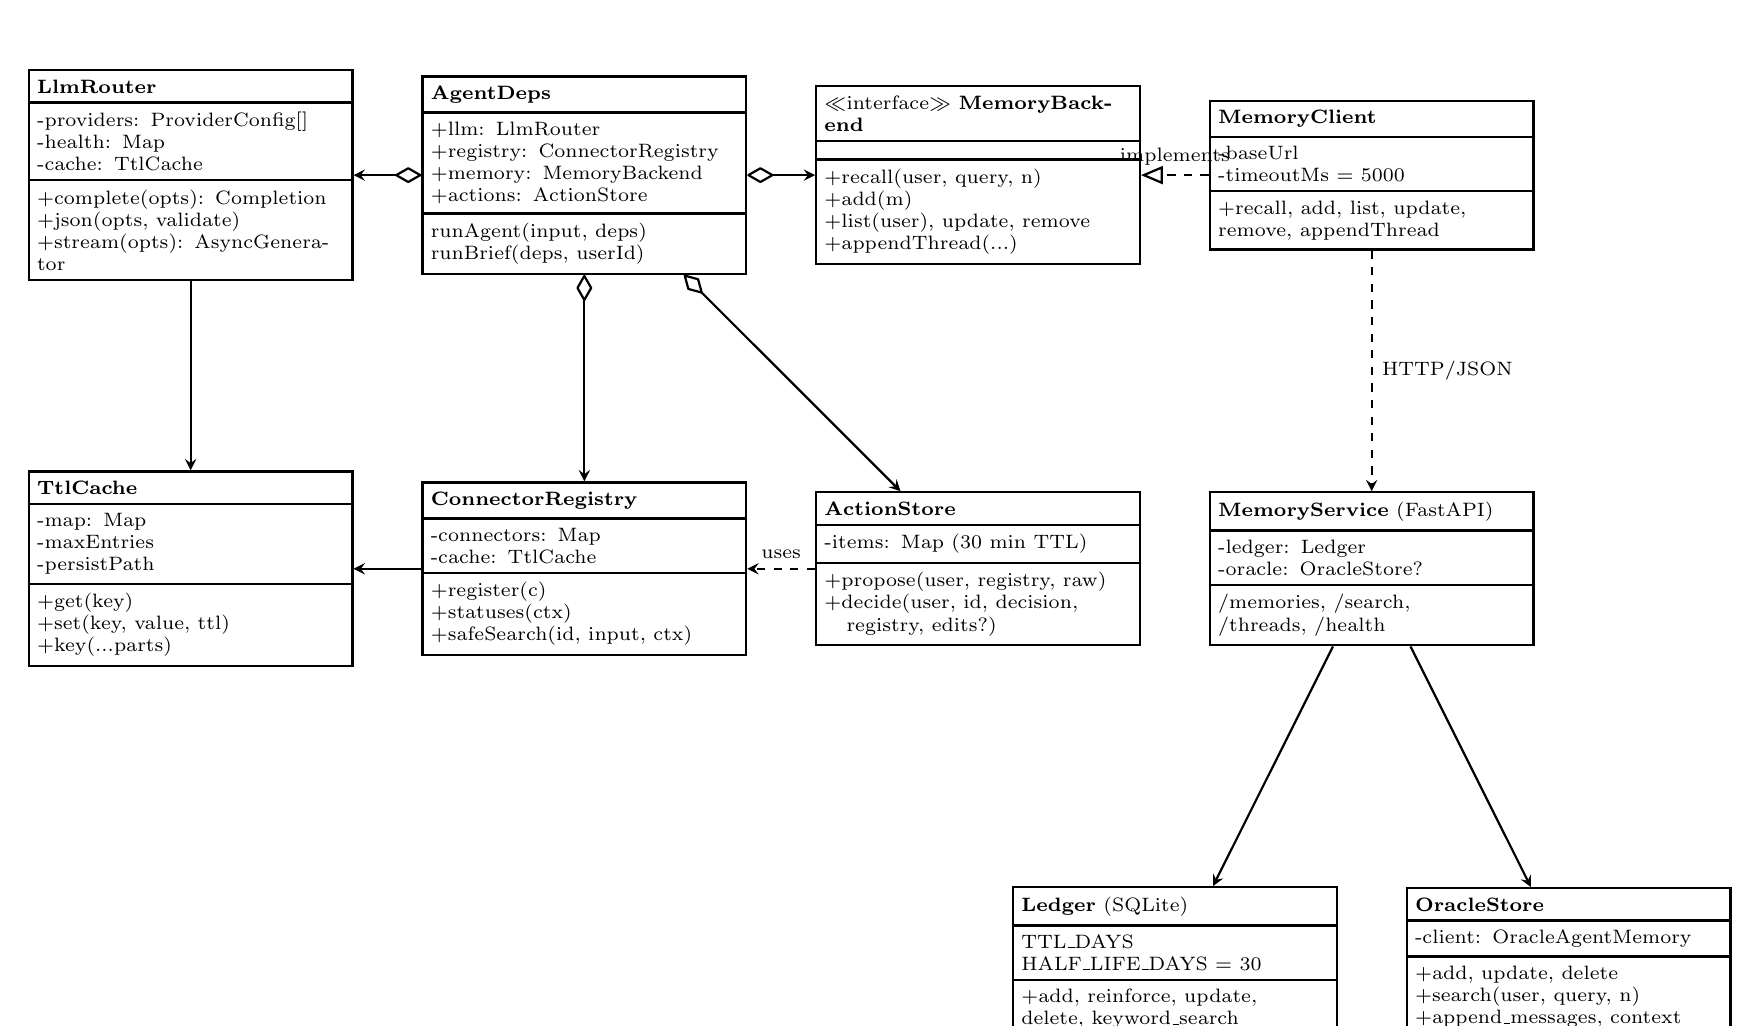
\begin{tikzpicture}[>=stealth, thick,
  cls/.style={draw, rectangle split, rectangle split parts=3, align=left, font=\scriptsize, inner sep=3pt, fill=white, text width=3.9cm, rectangle split part fill={blue!8,white,white}}]
\node[cls] (router) at (0,0) {\textbf{LlmRouter}\nodepart{second}-providers: ProviderConfig[]\\-health: Map\\-cache: TtlCache\nodepart{third}+complete(opts): Completion\\+json(opts, validate)\\+stream(opts): AsyncGenerator};
\node[cls] (deps) at (5,0) {\textbf{AgentDeps}\nodepart{second}+llm: LlmRouter\\+registry: ConnectorRegistry\\+memory: MemoryBackend\\+actions: ActionStore\nodepart{third}runAgent(input, deps)\\runBrief(deps, userId)};
\node[cls] (membe) at (10,0) {$\ll$interface$\gg$ \textbf{MemoryBackend}\nodepart{second}\mbox{}\nodepart{third}+recall(user, query, n)\\+add(m)\\+list(user), update, remove\\+appendThread(...)};
\node[cls] (memcl) at (15,0) {\textbf{MemoryClient}\nodepart{second}-baseUrl\\-timeoutMs = 5000\nodepart{third}+recall, add, list, update,\\remove, appendThread};
\node[cls] (cache) at (0,-5) {\textbf{TtlCache}\nodepart{second}-map: Map\\-maxEntries\\-persistPath\nodepart{third}+get(key)\\+set(key, value, ttl)\\+key(...parts)};
\node[cls] (reg) at (5,-5) {\textbf{ConnectorRegistry}\nodepart{second}-connectors: Map\\-cache: TtlCache\nodepart{third}+register(c)\\+statuses(ctx)\\+safeSearch(id, input, ctx)};
\node[cls] (store) at (10,-5) {\textbf{ActionStore}\nodepart{second}-items: Map (30 min TTL)\nodepart{third}+propose(user, registry, raw)\\+decide(user, id, decision,\\\quad registry, edits?)};
\node[cls] (svc) at (15,-5) {\textbf{MemoryService} (FastAPI)\nodepart{second}-ledger: Ledger\\-oracle: OracleStore?\nodepart{third}/memories, /search,\\/threads, /health};
\node[cls] (ledger) at (12.5,-10) {\textbf{Ledger} (SQLite)\nodepart{second}TTL\_DAYS\\HALF\_LIFE\_DAYS = 30\nodepart{third}+add, reinforce, update,\\delete, keyword\_search};
\node[cls] (ora) at (17.5,-10) {\textbf{OracleStore}\nodepart{second}-client: OracleAgentMemory\nodepart{third}+add, update, delete\\+search(user, query, n)\\+append\_messages, context};
\draw[open diamond->] (deps) -- (router);
\draw[open diamond->] (deps) -- (membe);
\draw[open diamond->] (deps) -- (reg);
\draw[open diamond->] (deps) -- (store);
\draw[dashed, ->] (store) -- node[above, font=\scriptsize] {uses} (reg);
\draw[dashed, -open triangle 45] (memcl) -- node[above, font=\scriptsize] {implements} (membe);
\draw[->] (router) -- (cache);
\draw[->] (reg) -- (cache);
\draw[dashed, ->] (memcl) -- node[right, font=\scriptsize] {HTTP/JSON} (svc);
\draw[->] (svc) -- (ledger);
\draw[->] (svc) -- (ora);
\end{tikzpicture}}}
		\caption{Agent, model router, actions and memory}
		\end{subfigure}

		\vspace{0.4cm}
		\begin{subfigure}{\textwidth}
		\centering
		\fbox{\resizebox{0.97\textwidth}{!}{%
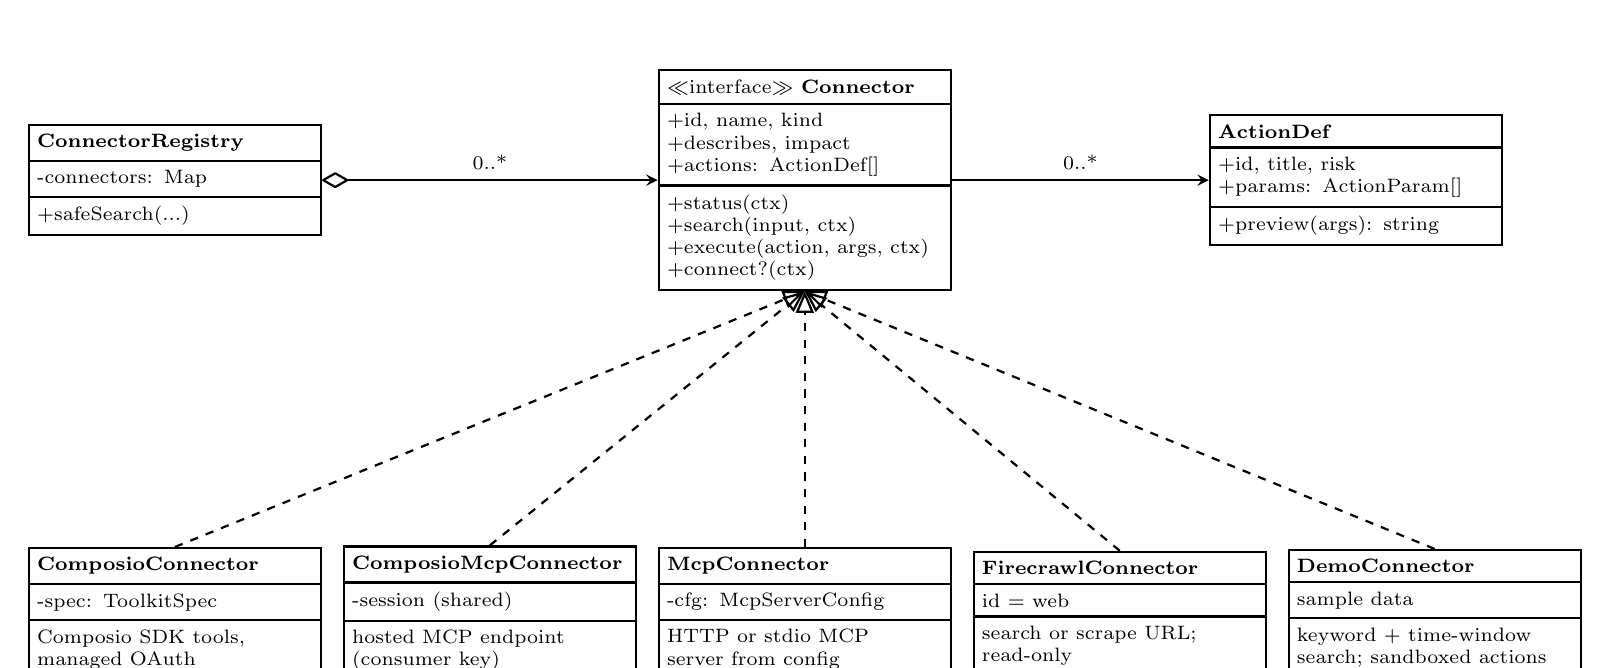
\begin{tikzpicture}[>=stealth, thick,
  cls/.style={draw, rectangle split, rectangle split parts=3, align=left, font=\scriptsize, inner sep=3pt, fill=white, text width=3.5cm, rectangle split part fill={blue!8,white,white}}]
\node[cls] (reg) at (0,0) {\textbf{ConnectorRegistry}\nodepart{second}-connectors: Map\nodepart{third}+safeSearch(...)};
\node[cls] (conn) at (8,0) {$\ll$interface$\gg$ \textbf{Connector}\nodepart{second}+id, name, kind\\+describes, impact\\+actions: ActionDef[]\nodepart{third}+status(ctx)\\+search(input, ctx)\\+execute(action, args, ctx)\\+connect?(ctx)};
\node[cls] (adef) at (15,0) {\textbf{ActionDef}\nodepart{second}+id, title, risk\\+params: ActionParam[]\nodepart{third}+preview(args): string};
\node[cls] (c1) at (0,-5.5) {\textbf{ComposioConnector}\nodepart{second}-spec: ToolkitSpec\nodepart{third}Composio SDK tools,\\managed OAuth};
\node[cls] (c2) at (4,-5.5) {\textbf{ComposioMcpConnector}\nodepart{second}-session (shared)\nodepart{third}hosted MCP endpoint\\(consumer key)};
\node[cls] (c3) at (8,-5.5) {\textbf{McpConnector}\nodepart{second}-cfg: McpServerConfig\nodepart{third}HTTP or stdio MCP\\server from config};
\node[cls] (c4) at (12,-5.5) {\textbf{FirecrawlConnector}\nodepart{second}id = web\nodepart{third}search or scrape URL;\\read-only};
\node[cls] (c5) at (16,-5.5) {\textbf{DemoConnector}\nodepart{second}sample data\nodepart{third}keyword + time-window\\search; sandboxed actions};
\draw[open diamond->] (reg) -- node[above, font=\scriptsize] {0..*} (conn);
\draw[->] (conn) -- node[above, font=\scriptsize] {0..*} (adef);
\foreach \cc in {c1,c2,c3,c4,c5} \draw[dashed, -open triangle 45] (\cc.north) -- (conn.south);
\end{tikzpicture}}}
		\caption{Connector layer}
		\end{subfigure}
	  \caption{Class Diagram}
	  \label{fig:class-dig}
	\end{figure}
\end{center}

\subsection{Interaction diagram for a consent-gated action}
Figure~\ref{fig:seq} shows the sequence of messages from a question that asks for an action to its execution. The agent's run ends after the proposal is stored; execution happens in a separate request, triggered only by the user.

\begin{figure}[!htbp]
\centering
\resizebox{\textwidth}{!}{%
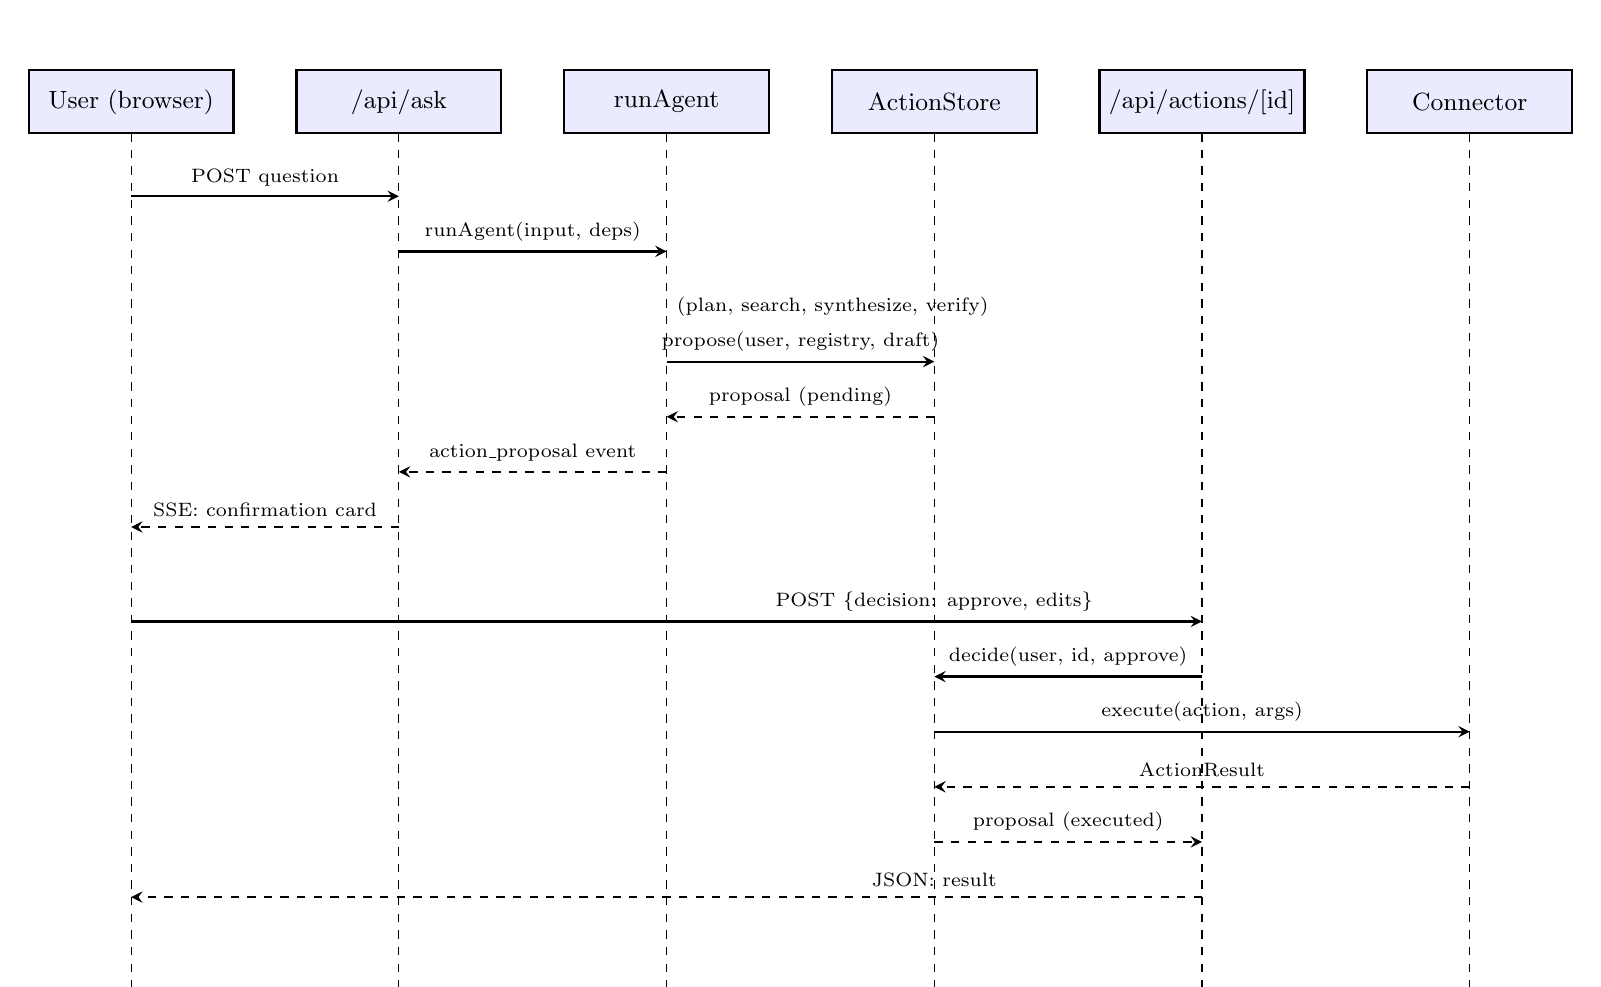
\begin{tikzpicture}[>=stealth, thick,
  hd/.style={draw, fill=blue!8, minimum width=2.6cm, minimum height=0.8cm, align=center, font=\small},
  msg/.style={->, font=\scriptsize},
  ret/.style={->, dashed, font=\scriptsize}]
\foreach \x/\n in {0/User (browser), 3.4/{/api/ask}, 6.8/runAgent, 10.2/ActionStore, 13.6/{/api/actions/[id]}, 17/Connector}
  { \node[hd] at (\x,0) {\n}; \draw[dashed, thin] (\x,-0.4) -- (\x,-11.4); }
\draw[msg] (0,-1.2) -- node[above] {POST question} (3.4,-1.2);
\draw[msg] (3.4,-1.9) -- node[above] {runAgent(input, deps)} (6.8,-1.9);
\node[font=\scriptsize, right] at (6.8,-2.6) {(plan, search, synthesize, verify)};
\draw[msg] (6.8,-3.3) -- node[above] {propose(user, registry, draft)} (10.2,-3.3);
\draw[ret] (10.2,-4.0) -- node[above] {proposal (pending)} (6.8,-4.0);
\draw[ret] (6.8,-4.7) -- node[above] {action\_proposal event} (3.4,-4.7);
\draw[ret] (3.4,-5.4) -- node[above] {SSE: confirmation card} (0,-5.4);
\draw[msg] (0,-6.6) -- node[above, pos=0.75] {POST \{decision: approve, edits\}} (13.6,-6.6);
\draw[msg] (13.6,-7.3) -- node[above] {decide(user, id, approve)} (10.2,-7.3);
\draw[msg] (10.2,-8.0) -- node[above] {execute(action, args)} (17,-8.0);
\draw[ret] (17,-8.7) -- node[above] {ActionResult} (10.2,-8.7);
\draw[ret] (10.2,-9.4) -- node[above] {proposal (executed)} (13.6,-9.4);
\draw[ret] (13.6,-10.1) -- node[above, pos=0.25] {JSON: result} (0,-10.1);
\end{tikzpicture}}
\caption{Sequence diagram of a consent-gated action}
\label{fig:seq}
\end{figure}


\chapter{Project Implementation}
\label{ch:impl}
  \section{Introduction}
Cortex is implemented as a TypeScript monorepository with npm workspaces (\texttt{apps/web}, \texttt{packages/agent}, \texttt{packages/connectors}, \texttt{packages/llm}, \texttt{packages/shared}) and a Python memory service (\texttt{services/memory}), together with an evaluation harness (\texttt{evals}) and helper scripts (\texttt{scripts}). The delivered code is about 6.1 thousand non-blank lines. This chapter lists the tools and technologies used and gives the main algorithms in pseudo code; every algorithm corresponds directly to code in the repository.
  \section{Tools and Technologies Used}
\begin{table}[!htbp]
\begin{center}
\def\arraystretch{1.25}
\small
\begin{tabularx}{\textwidth}{| p{3.4cm} | p{4.2cm} | X |}
\hline
Layer & Technology & Use in Cortex \\ \hline
Web application & Next.js 16, React 19, TypeScript & Screens, API route handlers, server-sent event streaming \\ \hline
Styling and motion & Tailwind CSS 4, Motion, Lucide icons & Interface styling, trace reveal animations, icons \\ \hline
Validation & Zod & Schemas for the plan, memory candidates, verification and brief outputs \\ \hline
Model access & OpenAI-compatible client & One client for Groq, Gemini, Cerebras, OpenRouter and Puter \\ \hline
Connectors & Composio SDK, MCP TypeScript SDK, Firecrawl SDK & Six work apps with managed OAuth; any MCP server; web search and scraping \\ \hline
Memory service & Python 3.11, FastAPI, Uvicorn, Pydantic, SQLite (FTS5) & Memory API, ledger and keyword search \\ \hline
Optional memory backend & Oracle AI Database, \texttt{oracledb}, Oracle Agent Memory & Vector search over memories, conversation threads \\ \hline
Observability & LangSmith SDK & Optional traces: run, model calls, searches \\ \hline
Testing & Vitest; \texttt{tsx} evaluation runner & 18 automated tests; 12-question evaluation \\ \hline
Interface review & Playwright (screenshots) & Desktop and mobile screenshots used in Chapter~\ref{ch:results} \\ \hline
\end{tabularx}
\end{center}
\caption{Tools and technologies}
\label{tab:tools}
\end{table}

  \section{Methodologies/Algorithm Details}
The orchestration follows a plan-then-execute methodology with fixed budgets. Algorithm~\ref{alg:run} is the agent run, Algorithm~\ref{alg:verify} the claim verification, Algorithm~\ref{alg:router} the model router's failover, and Algorithm~\ref{alg:memory} the memory policy.
  \subsection{Algorithm 1/Pseudo Code}
\begin{algorithm}[H]
\caption{Bounded agent run (runAgent)}
\label{alg:run}
\KwIn{question $q$, mode $m$, user $u$, history $H$}
\KwOut{ordered stream of typed events}
$C \leftarrow$ connected sources\; emit a failure event (source, reason, impact) for each unavailable source\;
$M \leftarrow$ recall$(u, q, 5)$ \tcp*{pinned memories always included}
\eIf{$m = \mathit{fast}$ \textbf{or} $C = \emptyset$}{
  $\Pi \leftarrow$ one sub-question over all sources (web only if hinted), keywords of $q$, locally parsed time window\;
}{
  $\Pi \leftarrow$ JSON plan from the fast model tier, validated and limited to 5 sub-questions over known sources\;
  \If{the output is unusable}{$\Pi \leftarrow$ the local single-step plan\;}
}
\If{intent$(\Pi) = \mathit{chat}$}{stream a short reply without retrieval\; \KwRet{}\;}
$T \leftarrow$ deduplicated pairs (source, query) of all sub-questions, $|T| \le 18$\;
run safeSearch for every $t \in T$ concurrently; collect evidence $E$; emit one failure event per failed source\;
\If{$m = \mathit{deep}$}{
  \ForEach{sub-question without evidence}{search its working sources again with the first two keywords and no time window, within the remaining tool budget\;}
}
$E^{*} \leftarrow$ the top $k$ items of $E$ by score after deduplication ($k = 16$ Deep, $8$ Fast), numbered $e_1, e_2, \ldots$\;
\If{$E^{*} = \emptyset$}{emit an honest ``not found'' answer naming the sources searched, without a model call\; \KwRet{}\;}
stream the synthesis (strong tier in Deep mode, fast tier in Fast mode), forwarding tokens only up to the first section marker\;
split the output into answer, conflicts, missing, actions, memory and follow-ups\;
$(L, G) \leftarrow$ VerifyClaims$(\mathit{answer}, E^{*})$\;
\If{$m = \mathit{deep}$ \textbf{and} some cited claims are not supported \textbf{and} the model budget allows}{
 re-judge up to 8 doubtful claims with the fast tier; keep the lexical verdicts if this fails\;}
emit the verdict: claims, $G$, conflicts mapped to evidence, missing items, follow-ups\;
\ForEach{action draft (at most 3)}{\If{ActionStore.propose succeeds}{emit the proposal with status pending\;}}
write explicit ``remember'' requests (salience 0.95) and model candidates with salience $\ge 0.6$, at most 2\;
append the turn to the conversation thread; emit usage and done\;
\end{algorithm}

  \subsection{Algorithm 2/Pseudo Code}
\begin{algorithm}[H]
\caption{Claim verification and groundedness (VerifyClaims)}
\label{alg:verify}
\KwIn{answer $A$, ranked evidence $E^{*}$}
\KwOut{claims $L$, groundedness $G$}
$L \leftarrow \emptyset$; $P \leftarrow \emptyset$ \tcp*{evidence cited by the previous sentence}
\ForEach{claim unit $c$ of $A$ (sentences and list items; code, quotes and remarks about Cortex's own drafts excluded)}{
  $R \leftarrow$ the citation numbers $[n]$ in $c$\;
  \eIf{$R = \emptyset$}{
    \If{$c$ states no fact \textbf{or} $c$ is a hedge (e.g. ``the evidence does not mention'')}{skip $c$\;}
    \eIf{$P \neq \emptyset$ \textbf{and} Score$(c, P) = \mathit{supported}$}{append $(c, P, \mathit{supported})$ to $L$\;}{append $(c, \emptyset, \mathit{unsupported})$ to $L$\;}
  }{
    $E_c \leftarrow \{E^{*}_n : n \in R\}$\;
    \eIf{$E_c = \emptyset$}{append $(c, \emptyset, \mathit{unsupported})$ to $L$\;}{$P \leftarrow E_c$; append $(c, E_c, \mathrm{Score}(c, E_c))$ to $L$\;}
  }
}
$G \leftarrow 1$ if $L = \emptyset$, otherwise $\frac{1}{|L|}\sum_{c \in L} w(c)$ with $w = 1, 0.5, 0$\;
\KwRet{$(L, G)$}\;
\BlankLine
\textbf{Score}$(c, E_c)$: $T(\cdot)$ lower-cases, removes stop words and short tokens and strips common suffixes\;
$o \leftarrow |T(c) \cap T(E_c)| \,/\, |T(c)|$; \textit{numbersOk} $\leftarrow$ every number in $c$ occurs in $E_c$\;
\KwRet{supported if $o \ge 0.4$ and numbersOk; partial if $o \ge 0.2$; unsupported otherwise}\;
\end{algorithm}

\subsection{Algorithm 3/Pseudo Code}
\begin{algorithm}[H]
\caption{Free-tier model router with failover (LlmRouter.complete)}
\label{alg:router}
\KwIn{tier (strong or fast), messages, options}
\KwOut{completion, or LlmUnavailableError}
$key \leftarrow$ SHA-256 of (tier, messages, JSON flag, token limit)\;
\If{the cache holds a live entry for $key$}{\KwRet{the cached completion (marked cached)}\;}
\For{$round \leftarrow 1$ \KwTo $2$}{
  \If{$round = 2$}{wait for the provider that recovers soonest if that is within 12~s; otherwise stop\;}
  \ForEach{provider $p$ not cooling down, in order (free tiers first, Puter last)}{
    request the model of the tier from $p$ (25~s timeout)\;
    \eIf{the reply is non-empty and, if JSON was requested, parseable}{reset the health of $p$; cache the reply (default 6~h)\; \KwRet{the reply}\;}{
      cooldown of $p$: rate limit (429) $\rightarrow$ retry-after or 60~s; invalid key (401/403) $\rightarrow$ 10~min; out of credit (402) $\rightarrow$ 1~h; model not found (404) $\rightarrow$ 10~min; otherwise $15~\mathrm{s} \times \min(\mathit{failures}, 4)$\;}
  }
}
raise LlmUnavailableError listing every provider and reason\;
\end{algorithm}
Streaming uses the same loop, but fails over only before the first token: a stream that breaks after it has started is reported honestly rather than silently restarted on another provider.

\subsection{Algorithm 4/Pseudo Code}
\begin{algorithm}[H]
\caption{Memory policy: write and recall}
\label{alg:memory}
\KwIn{memory candidate $m$ (user, content, kind, salience, reason, source, run); or a recall request $(u, q, n)$}
\textbf{Write}$(m)$:\;
\eIf{a live memory of the same user has similarity ratio $> 0.82$ with $m$}{reinforce it: salience $\leftarrow \max(\mathit{old}, \mathit{new})$, creation time $\leftarrow$ now\;}{
  insert $m$ with expiry from its kind (priority 45~d, decision 120~d, fact 90~d, person and preference never)\;
  if Oracle is configured, add it to Oracle Agent Memory with the same identifier\;}
\BlankLine
\textbf{Recall}$(u, q, n)$:\;
$R \leftarrow$ up to 3 pinned memories of $u$\;
$H \leftarrow$ Oracle vector search for $2n$ hits; if unavailable or empty, FTS5 BM25 search (or token overlap) for $2n$ hits\;
\ForEach{hit $h \in H$ not already in $R$, live and not expired}{
  $s_{\mathit{eff}} \leftarrow s$ if pinned, else $s \cdot 0.5^{\,\mathit{age}/30}$\;
  $\mathit{score}(h) \leftarrow \mathit{rel}(h) \cdot (0.5 + 0.5\, s_{\mathit{eff}})$\;
}
\KwRet{$R$ followed by the best $n - |R|$ hits by score}\;
\end{algorithm}

  \section{Verification and Validation for Acceptance}
The system is accepted against the goals and objectives of Section~\ref{sec:goals} with the following checks; Table~\ref{tab:acceptance} gives the status at the time of writing.

\begin{table}[!htbp]
\begin{center}
\def\arraystretch{1.25}
\small
\begin{tabularx}{\textwidth}{| X | p{4.2cm} | p{2.6cm} |}
\hline
Acceptance criterion & How it is checked & Status \\ \hline
Every factual sentence cites evidence; claims are verified & Verification unit test; groundedness in evaluation & Met (mean 0.88) \\ \hline
Expected facts are found in the cited evidence & Citation recall in evaluation & Met (0.92) \\ \hline
Unanswerable questions are answered honestly & ``Not found'' unit test and evaluation case & Met (1/1) \\ \hline
No action executes without explicit approval & ActionStore and Fast Mode unit tests; evaluation check & Met (0 executions without consent) \\ \hline
Cross-source conflicts are reported & Unit test; two evaluation cases & Partly met (1/2) \\ \hline
Requested actions are proposed & Two evaluation cases & Partly met (1/2) \\ \hline
A failed source is named and the run continues & Integration test with a failing connector & Met \\ \hline
Model provider failure is handled & Router failover and cooldown tests & Met \\ \hline
Fast Mode uses one model call & Unit test & Met \\ \hline
Real services work with real keys & Live checks of Groq, Gemini (Flash-Lite), Firecrawl, LangSmith and Composio hosted MCP & Met \\ \hline
Oracle memory backend & Local Oracle AI Database Free container & Not met yet (SQLite fallback in use) \\ \hline
\end{tabularx}
\end{center}
\caption{Acceptance checks}
\label{tab:acceptance}
\end{table}


\chapter{Software Testing}
\label{ch:testing}
 \section{Type of Testing Used}
\begin{itemize}
\item \textbf{Unit testing} (Vitest): pure functions and single classes, such as JSON parsing, claim verification, section splitting, time-window parsing, evidence extraction and the action store.
\item \textbf{Integration testing} (Vitest): the model router against local stub HTTP servers that imitate providers (including a rate-limited one); the connector registry with a failing connector; and the whole agent run over the sample workspace with a stubbed model, checking the event stream end to end.
\item \textbf{System testing and evaluation}: the evaluation harness runs 12 questions end to end in Deep mode over the sample workspace with real free-tier models and measures groundedness, citation recall, conflict detection, honest ``not found'' answers, action proposals, execution without consent, and latency.
\item \textbf{Live service checks}: a script lists the models of every configured provider and sends a JSON request to each tier, verifies every Composio tool used by the toolkits, and checks Firecrawl, printing names and status only, never keys.
\item \textbf{Interface review}: desktop and mobile screenshots of every screen were reviewed against the design brief, and the issues found were fixed in two review rounds.
\end{itemize}
   \section{Test Cases and Test Results}
All 18 automated tests pass. Tables~\ref{tab:test-llm}, \ref{tab:test-conn} and~\ref{tab:test-agent} list them by package. The evaluation results follow in Table~\ref{tab:eval}.

\begin{table}[!htbp]
\begin{center}
\def\arraystretch{1.25}
\small
\begin{tabularx}{\textwidth}{| c | X | X | c |}
\hline
ID & Test case & Expected result & Result \\ \hline
TL1 & Two providers, the first returns HTTP 429; then a second request & Answer comes from the healthy provider; the limited provider is not called again while cooling down & Pass \\ \hline
TL2 & The same prompt is sent twice & Second answer is served from the cache; the provider is called once & Pass \\ \hline
TL3 & No provider is configured & \texttt{LlmUnavailableError} is raised & Pass \\ \hline
TL4 & JSON inside a code fence, or embedded in prose & Both are parsed into the same object & Pass \\ \hline
\end{tabularx}
\end{center}
\caption{Test cases: model router (packages/llm)}
\label{tab:test-llm}
\end{table}

\begin{table}[!htbp]
\begin{center}
\def\arraystretch{1.25}
\small
\begin{tabularx}{\textwidth}{| c | X | X | c |}
\hline
ID & Test case & Expected result & Result \\ \hline
TC1 & Search Slack and GitHub of the sample workspace for Demo Day & Slack says Demo Day moved; GitHub returns the milestone (the planted conflict) & Pass \\ \hline
TC2 & Empty query with a one-week time window & Recent items are returned instead of nothing & Pass \\ \hline
TC3 & Execute ``send email'' on the sample Gmail connector & Recorded in the sandbox; message says nothing left the sample workspace & Pass \\ \hline
TC4 & A connector whose search always fails with ``fetch failed'' & Failure names Slack, reason ``could not be reached'', impact about blockers; exactly two attempts & Pass \\ \hline
TC5 & Nested tool output (data, messages, subject, text, timestamp, sender) & Evidence with title, quote, author and normalised timestamp & Pass \\ \hline
\end{tabularx}
\end{center}
\caption{Test cases: connectors (packages/connectors)}
\label{tab:test-conn}
\end{table}

\begin{table}[!htbp]
\begin{center}
\def\arraystretch{1.25}
\small
\begin{tabularx}{\textwidth}{| c | X | X | c |}
\hline
ID & Test case & Expected result & Result \\ \hline
TA1 & Fast Mode run over the sample workspace with a stub model & Exactly one model call; plan and tool calls emitted; no section markers reach the user; one conflict; proposal pending; stream ends with done & Pass \\ \hline
TA2 & Run with Slack failing & A source error names Slack; an answer is still produced & Pass \\ \hline
TA3 & Question with no matching evidence & ``Couldn't find'' answer; zero model calls & Pass \\ \hline
TA4 & ``Remember that Orbit is my top priority \ldots'' & The memory is written & Pass \\ \hline
TA5 & Claims with a correct number, a wrong number, and no citation & supported, partial, unsupported & Pass \\ \hline
TA6 & Synthesis output with sections; stream ending in a partial marker & One action parsed; partial marker held back & Pass \\ \hline
TA7 & ``this week'', ``upcoming deadlines'', ``hello'' & last 7 days, next 30 days, no window & Pass \\ \hline
TA8 & Approve by another user; approve by the owner; approve again & Refused; executed; refused as already executed & Pass \\ \hline
TA9 & Proposal missing a required field & Rejected naming the missing field & Pass \\ \hline
\end{tabularx}
\end{center}
\caption{Test cases: agent, verification and actions (packages/agent)}
\label{tab:test-agent}
\end{table}

\textbf{Evaluation.} The evaluation used Deep mode over the fictional sample workspace with free-tier models: Groq \texttt{openai/gpt-oss-120b} as the primary strong model (with \texttt{gpt-oss-20b} as the fast tier) and Gemini 3.5 Flash-Lite as the fallback. Questions were spaced six seconds apart. Because the router tries Groq first, the eight questions answered by Gemini are those for which Groq was rate-limited or failing at that moment. Table~\ref{tab:eval} gives the per-question results. These results are \emph{preliminary}: twelve questions over one small fictional workspace are not a benchmark, and repeated runs differ (conflict detection in particular varied between runs).

\begin{table}[!htbp]
\begin{center}
\def\arraystretch{1.2}
\small
\begin{tabular}{| l | c | c | c | c | c |}
\hline
Question ID & Groundedness & Citation recall & Specific check & Time (s) & Answered by \\ \hline
demo-day-change & 0.89 & 1.00 & conflict: yes & 5.4 & Groq \\ \hline
blockers & 1.00 & 1.00 & -- & 7.1 & Gemini \\ \hline
login-bug & 0.81 & 1.00 & -- & 3.7 & Groq \\ \hline
report-due & 0.67 & 0.50 & -- & 4.7 & Gemini \\ \hline
oa-deadline & 0.50 & 0.50 & -- & 3.3 & Gemini \\ \hline
user-testing & 1.00 & 1.00 & -- & 3.5 & Groq \\ \hline
chat-scope & 1.00 & 1.00 & -- & 8.0 & Gemini \\ \hline
oss-pr & 0.67 & 1.00 & -- & 2.8 & Gemini \\ \hline
risks-week & 1.00 & 1.00 & conflict: no & 4.9 & Gemini \\ \hline
unknown & 1.00 & 1.00 & not found: yes & 2.4 & Gemini \\ \hline
action-slack & 1.00 & 1.00 & action: yes & 2.4 & Gemini \\ \hline
action-email & 1.00 & 1.00 & action: no & 3.2 & Gemini \\ \hline
\textbf{Summary} & \textbf{0.88} & \textbf{0.92} & see text & p50 3.7, p90 7.1 & \\ \hline
\end{tabular}
\end{center}
\caption{Preliminary evaluation results (Deep mode, 12 questions)}
\label{tab:eval}
\end{table}

Summary of the evaluation: mean groundedness 0.88; citation recall 0.92; honest ``not found'' 1/1; action proposals 1/2; conflict detection 1/2; zero actions executed without consent; median latency 3.7~s and 90th percentile 7.1~s. Citation recall is the fraction of expected key facts that appear in the evidence the answer actually cites.

\chapter{Results}
\label{ch:results}
\section{Screen shots}
The screenshots below show the main screens over the sample workspace. They were captured for the interface review with the development mock model, which quotes evidence verbatim, so they show the interface and its states rather than the quality of a real model's answer; the measured quality is reported in Section~\ref{sec:outputs}.

\begin{figure}[!htbp]
\centering
\fbox{\includegraphics[width=0.95\textwidth]{screens/ask.png}}
\caption{Ask screen: a cited answer with a struck-through unsupported claim, a reported conflict between two sources, and the cited sources}
\label{fig:ss-ask}
\end{figure}

\begin{figure}[!htbp]
\centering
\fbox{\includegraphics[width=0.95\textwidth]{screens/trace.png}}
\caption{Live trace: step timings, the three-step plan and each tool call with its query, result count and latency}
\label{fig:ss-trace}
\end{figure}

\begin{figure}[!htbp]
\centering
\fbox{\includegraphics[width=0.95\textwidth]{screens/action.png}}
\caption{A proposed Slack message waiting for approval, with an exact preview and Edit, Decline and Approve controls}
\label{fig:ss-action}
\end{figure}

\begin{figure}[!htbp]
\centering
\fbox{\includegraphics[width=0.8\textwidth]{screens/brief.png}}
\caption{Daily Brief: at-risk items, conflicts, upcoming deadlines and recent changes, each linked to its sources}
\label{fig:ss-brief}
\end{figure}

\begin{figure}[!htbp]
\centering
\fbox{\includegraphics[width=0.95\textwidth]{screens/memory.png}}
\caption{Memory inspector (empty state) with the control to teach Cortex a memory of a chosen kind}
\label{fig:ss-memory}
\end{figure}

\begin{figure}[!htbp]
\centering
\fbox{\includegraphics[width=0.95\textwidth]{screens/connections.png}}
\caption{Connections: the sample workspace with six sources, and the language model and memory status}
\label{fig:ss-connections}
\end{figure}

\begin{figure}[!htbp]
\centering
\begin{subfigure}{0.45\textwidth}
\centering
\fbox{\includegraphics[height=9cm]{screens/ask-mobile.png}}
\caption{Ask}
\end{subfigure}
\begin{subfigure}{0.45\textwidth}
\centering
\fbox{\includegraphics[height=9cm]{screens/brief-mobile.png}}
\caption{Brief}
\end{subfigure}
\caption{Mobile layout}
\label{fig:ss-mobile}
\end{figure}

\section{Outputs}
\label{sec:outputs}
The outputs of the system for one question are: the streamed answer with numbered citations; the verdict (status of each claim, groundedness, conflicts, missing items, follow-up questions); any action proposals; any memories written; and the usage record (model calls, cached calls, tool calls, time, models used). Figures~\ref{fig:chart-g} and~\ref{fig:chart-t} summarise the measured outputs of the preliminary evaluation in Table~\ref{tab:eval}.

\begin{figure}[!htbp]
\centering
\resizebox{\textwidth}{!}{%
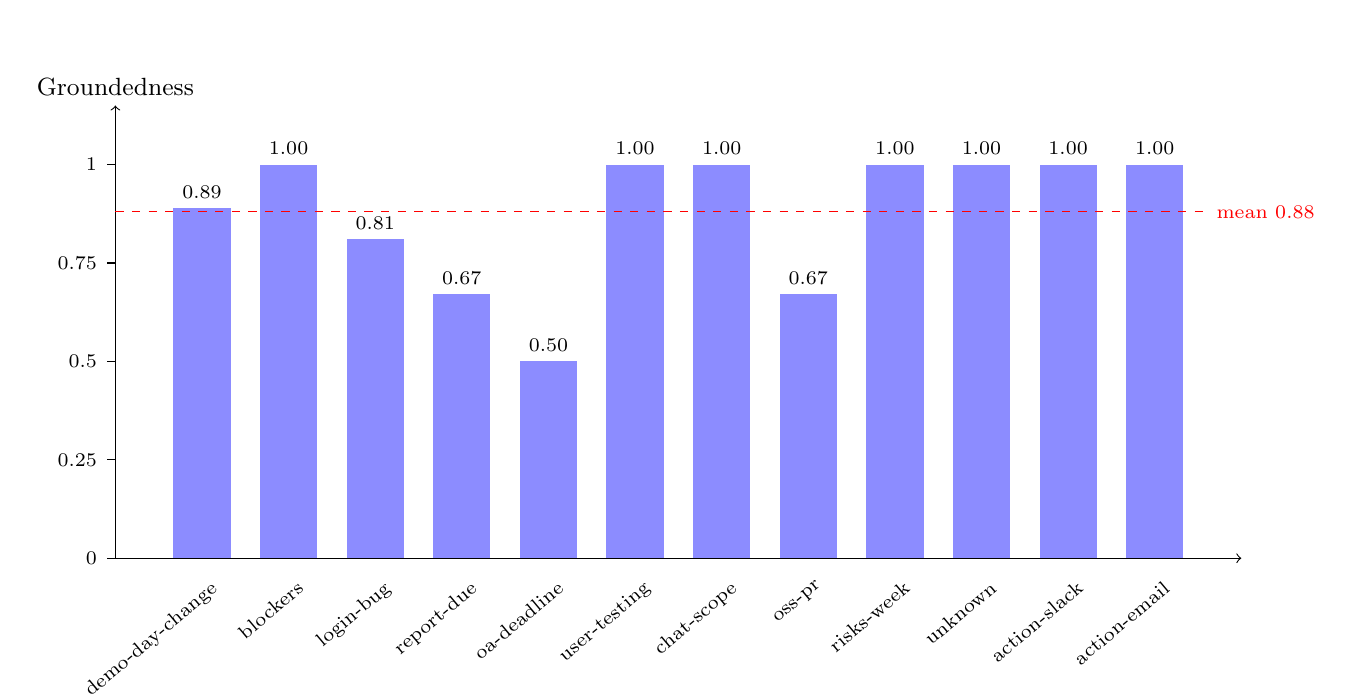
\begin{tikzpicture}[x=1.1cm, y=5cm]
\draw[->] (0,0) -- (13,0);
\draw[->] (0,0) -- (0,1.15) node[above, font=\small] {Groundedness};
\foreach \yv in {0,0.25,0.5,0.75,1} \draw (0,\yv) -- (-0.1,\yv) node[left, font=\scriptsize] {\yv};
\foreach \bi/\bv/\bn in {1/0.89/demo-day-change, 2/1.00/blockers, 3/0.81/login-bug, 4/0.67/report-due, 5/0.50/oa-deadline, 6/1.00/user-testing, 7/1.00/chat-scope, 8/0.67/oss-pr, 9/1.00/risks-week, 10/1.00/unknown, 11/1.00/action-slack, 12/1.00/action-email}
{
  \fill[blue!45] (\bi-0.33,0) rectangle (\bi+0.33,\bv);
  \node[font=\scriptsize, above] at (\bi,\bv) {\bv};
  \node[font=\scriptsize, rotate=40, anchor=north east] at (\bi+0.1,-0.02) {\bn};
}
\draw[dashed, red] (0,0.88) -- (12.6,0.88) node[right, font=\scriptsize] {mean 0.88};
\end{tikzpicture}}
\caption{Groundedness per evaluation question}
\label{fig:chart-g}
\end{figure}

\begin{figure}[!htbp]
\centering
\resizebox{\textwidth}{!}{%
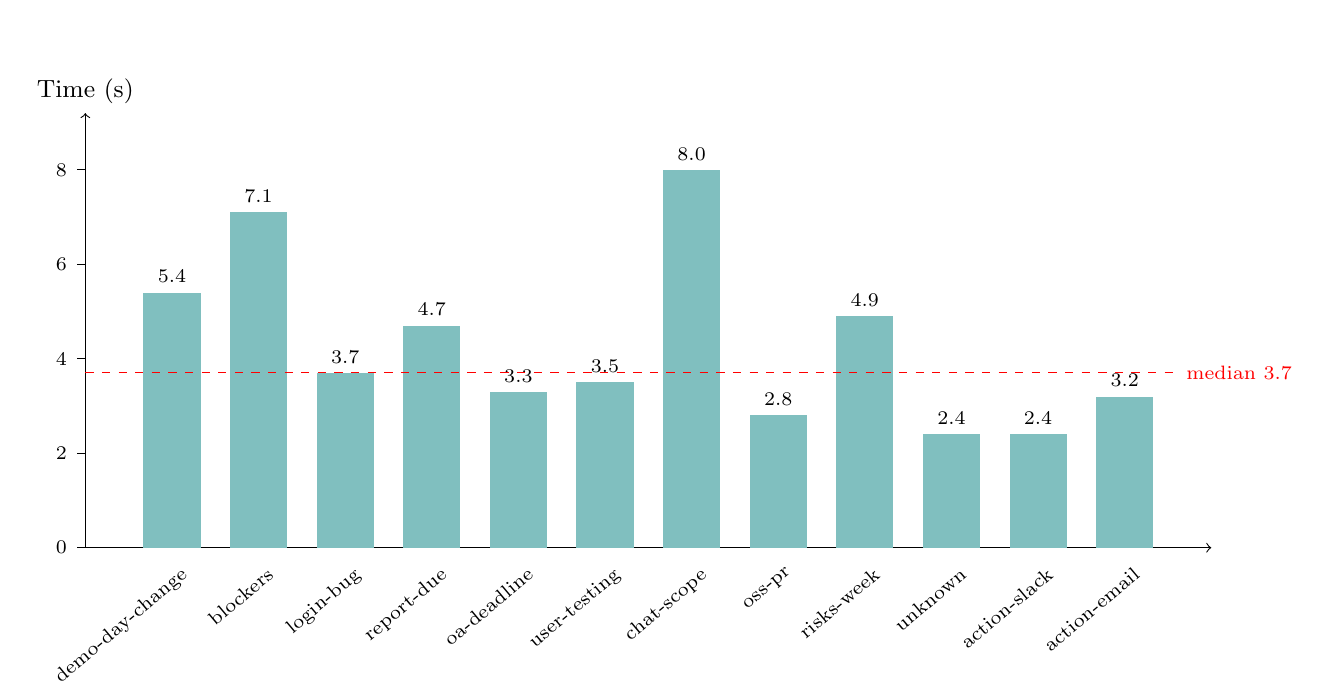
\begin{tikzpicture}[x=1.1cm, y=0.6cm]
\draw[->] (0,0) -- (13,0);
\draw[->] (0,0) -- (0,9.2) node[above, font=\small] {Time (s)};
\foreach \yv in {0,2,4,6,8} \draw (0,\yv) -- (-0.1,\yv) node[left, font=\scriptsize] {\yv};
\foreach \bi/\bv/\bn in {1/5.4/demo-day-change, 2/7.1/blockers, 3/3.7/login-bug, 4/4.7/report-due, 5/3.3/oa-deadline, 6/3.5/user-testing, 7/8.0/chat-scope, 8/2.8/oss-pr, 9/4.9/risks-week, 10/2.4/unknown, 11/2.4/action-slack, 12/3.2/action-email}
{
  \fill[teal!50] (\bi-0.33,0) rectangle (\bi+0.33,\bv);
  \node[font=\scriptsize, above] at (\bi,\bv) {\bv};
  \node[font=\scriptsize, rotate=40, anchor=north east] at (\bi+0.1,-0.1) {\bn};
}
\draw[dashed, red] (0,3.7) -- (12.6,3.7) node[right, font=\scriptsize] {median 3.7};
\end{tikzpicture}}
\caption{End-to-end time per evaluation question (Deep mode)}
\label{fig:chart-t}
\end{figure}

\textbf{Discussion.} Groundedness was 1.00 for seven of the twelve questions. The lowest values (0.50 and 0.67) came from questions about deadlines (``oa-deadline'', ``report-due''), where the answers added dates or details in sentences that the lexical check could not match to the cited evidence; these are also the two questions with a citation recall of 0.5. Of the two questions designed to expose the planted Demo Day conflict, the conflict was reported for the direct question but not for the broader weekly summary, and the behaviour varied between runs; conflict detection currently depends on the model writing the conflicts section, which is the main weakness to address. One of the two action requests was proposed; for the e-mail request, no Gmail proposal was produced in this run. In all twelve runs no action was executed, which is the property the design guarantees regardless of model behaviour. The unanswerable question about a company's Series B was answered as not found. Live tests with real keys confirmed that Groq, Gemini (Flash-Lite), Firecrawl, LangSmith and Composio's hosted MCP endpoint (consumer key) work with the system; the Oracle AI Database container was set up but could not be reached because of a Docker networking issue, so all memory results use the SQLite backend.

\chapter{Deployment and Maintenance}
\label{ch:deploy}
     \section{Installation and un-installation}
\textbf{Prerequisites:} Node.js 24 or later, npm, Python 3.11 and Git; optionally Docker for the local Oracle database.

\textbf{Installation:}
\begin{enumerate}
\item Obtain the source code and run \texttt{npm install} in the repository root.
\item Copy \texttt{.env.example} to \texttt{.env} and add at least one model key (for example \texttt{GEMINI\_API\_KEY} or \texttt{GROQ\_API\_KEY}). Optional keys: \texttt{COMPOSIO\_API\_KEY} (own accounts), \texttt{FIRECRAWL\_API\_KEY} (web), \texttt{LANGSMITH\_API\_KEY} (tracing), and the Oracle connection settings.
\item Run \texttt{npm run memory:setup} once to create the Python virtual environment of the memory service.
\item Start the memory service with \texttt{npm run memory} (port 8000) and, in a second terminal, the web application with \texttt{npm run dev} (\url{http://localhost:3000}).
\item Optional: \texttt{npm run oracle:local} starts a local Oracle AI Database Free container; set \texttt{ORACLE\_DB\_USER}, \texttt{ORACLE\_DB\_PASSWORD} and \texttt{ORACLE\_DB\_DSN} so that the memory service uses it.
\item Optional: to add an MCP server, copy \texttt{mcp.config.example.json} to \texttt{mcp.config.json}, edit it and set \texttt{CORTEX\_MCP\_CONFIG}.
\item Verification: \texttt{npm test} runs the 18 tests; \texttt{npm run eval} runs the evaluation; \texttt{npx tsx scripts/check-services.ts} checks the configured services.
\end{enumerate}
Without any keys, \texttt{npm run mock-llm} starts a development-only mock model; the application then uses it when \texttt{CORTEX\_MOCK\_LLM\_URL} is set.

\textbf{Un-installation:} stop both processes; delete the repository folder (this removes the dependencies, the virtual environment, the caches in \texttt{.cache} and the memory ledger in \texttt{services/memory/data}); if the Oracle container was created, remove it with \texttt{docker rm -f cortex-oracle} and its volume with \texttt{docker volume rm cortex-oradata}; revoke any API keys and Composio connections that are no longer needed.

\textbf{Maintenance:} free-tier catalogues change, so model identifiers are environment variables and the service check script reports missing models; Composio tool names are kept in one file; connector failures are visible in the interface and in optional LangSmith traces; and the evaluation is re-run after changes to prompts or models.
     \section{User help}
\begin{itemize}
\item \textbf{Ask:} type a question and press Enter. Choose \emph{Deep} (plans, searches in parallel, verifies every claim) or \emph{Fast} (single pass, quickest). Numbers in the answer are citations; select one to see its source. A claim drawn with a strike-through could not be matched to the sources. Conflicts and missing information are listed below the answer. Select \emph{Trace} to see the plan, the searches and their timings.
\item \textbf{Actions:} ask Cortex to draft or send something. It shows a card with the exact content; select \emph{Edit} to change it, \emph{Decline} to discard it or \emph{Approve} to run it once. Nothing is sent without this step.
\item \textbf{Brief:} open \emph{Brief} for what changed in the last week and what is due soon, with sources; select \emph{Ask} on a card to ask about it.
\item \textbf{Memory:} say ``remember that \ldots'' in a question, or use \emph{Teach Cortex something} on the Memory page. Each memory shows why it was kept; pin it to keep it from fading, edit it, or forget it.
\item \textbf{Connections:} use the sample workspace to try Cortex without accounts, or connect your own apps with one click (when the server has a Composio key).
\item \textbf{When something fails:} Cortex names the source that failed, why, and what may be missing from the answer, and continues with the others. If every model is busy, wait a minute or switch to Fast mode.
\end{itemize}

 \chapter{Conclusion and future scope}
\textbf{Summary.} This project designed and implemented Cortex, an agentic retrieval-augmented generation system over live work data. A bounded plan-then-execute pipeline decomposes each question, searches several sources in parallel through a uniform connector registry, streams an answer that must cite numbered evidence, verifies each claim, reports conflicts and missing information, proposes but never executes actions, and keeps a small, explainable memory. A free-tier model router with failover, cooldowns and caching keeps the operating cost at zero.

\textbf{Conclusion.} The preliminary results support the main design choices: a mean groundedness of 0.88 and a citation recall of 0.92 over twelve questions, an honest answer to the unanswerable question, a median end-to-end time of 3.7~s, and no action executed without consent in any run, a property that follows from the design rather than from model behaviour. The same evaluation shows where the system is weakest: conflict detection and action proposals succeeded in only one of two cases each, and deadline questions had the lowest groundedness. Following the base paper GRASP, which shows that the granularity and number of retrieval steps matter, Cortex keeps evidence small and retrieval bounded, but it does so with fixed rules rather than a learned policy.

\textbf{Future scope.}
\begin{itemize}
\item Make conflict detection independent of the synthesis model, for example by comparing dates and numbers extracted from evidence of different sources about the same entity.
\item Enlarge the evaluation to the planned 50 questions, repeat runs to report variance, and add citation precision.
\item Bring the Oracle AI Database backend into use for vector search over memories, and compare it with the SQLite keyword fallback.
\item Implement the remaining vision items: time-travel queries over source snapshots, an editable plan before execution, and shareable reasoning receipts.
\item Expose Cortex itself as an MCP server, so that other assistants can use its research and memory.
\item Study a learned, granularity-aware retrieval policy in the spirit of GRASP once a trainable model and data are available.
\item Deploy to a hosted environment with persistent storage for pending actions.
\end{itemize}

% \bibliographystyle{plain}

\bibliographystyle{ieeetr}
\bibliography{biblo}

\begin{appendices}

\chapter{References}
(Strictly in ACM Format)

The references cited in this report are listed below in the ACM reference format. The numbered list produced by BibTeX appears in the References chapter before the annexures.

\begin{enumerate}
\setlength{\itemsep}{2pt}
\small
\item Akari Asai, Zeqiu Wu, Yizhong Wang, Avirup Sil, and Hannaneh Hajishirzi. 2024. Self-RAG: Learning to Retrieve, Generate, and Critique through Self-Reflection. In \textit{The Twelfth International Conference on Learning Representations (ICLR 2024)}.
\item Michael Chui, James Manyika, Jacques Bughin, et al. 2012. \textit{The Social Economy: Unlocking Value and Productivity through Social Technologies}. McKinsey Global Institute.
\item Michael Chui, Eric Hazan, Roger Roberts, et al. 2023. \textit{The Economic Potential of Generative AI: The Next Productivity Frontier}. McKinsey \& Company.
\item Shahul Es, Jithin James, Luis Espinosa Anke, and Steven Schockaert. 2024. RAGAs: Automated Evaluation of Retrieval Augmented Generation. In \textit{Proceedings of the 18th Conference of the European Chapter of the Association for Computational Linguistics: System Demonstrations}. ACL, 150--158.
\item Varun Gandhi, Jaewook Lee, Shantanu Todmal, Franck Dernoncourt, Ryan Rossi, Zichao Wang, and Andrew Lan. 2026. GRASP: GRanularity-Aware Search Policy for Agentic RAG. arXiv:2607.10463.
\item Luyu Gao, Zhuyun Dai, Panupong Pasupat, Anthony Chen, Arun Tejasvi Chaganty, Yicheng Fan, Vincent Zhao, Ni Lao, Hongrae Lee, Da-Cheng Juan, and Kelvin Guu. 2023. RARR: Researching and Revising What Language Models Say, Using Language Models. In \textit{Proceedings of the 61st Annual Meeting of the Association for Computational Linguistics (Volume 1: Long Papers)}. ACL, 16477--16508.
\item Tianyu Gao, Howard Yen, Jiatong Yu, and Danqi Chen. 2023. Enabling Large Language Models to Generate Text with Citations. In \textit{Proceedings of the 2023 Conference on Empirical Methods in Natural Language Processing}. ACL, 6465--6488.
\item Xinyi Hou, Yanjie Zhao, Shenao Wang, and Haoyu Wang. 2025. Model Context Protocol (MCP): Landscape, Security Threats, and Future Research Directions. arXiv:2503.23278.
\item Soyeong Jeong, Jinheon Baek, Sukmin Cho, Sung Ju Hwang, and Jong C. Park. 2024. Adaptive-RAG: Learning to Adapt Retrieval-Augmented Large Language Models through Question Complexity. In \textit{Proceedings of the 2024 Conference of the North American Chapter of the Association for Computational Linguistics (NAACL 2024)}.
\item Bowen Jin, Hansi Zeng, Zhenrui Yue, Jinsung Yoon, Sercan Arik, Dong Wang, Hamed Zamani, and Jiawei Han. 2025. Search-R1: Training LLMs to Reason and Leverage Search Engines with Reinforcement Learning. arXiv:2503.09516.
\item Parag Kulkarni. 2015. \textit{Knowledge Innovation Strategy}. Bloomsbury Publishing India.
\item Patrick Lewis, Ethan Perez, Aleksandra Piktus, Fabio Petroni, Vladimir Karpukhin, Naman Goyal, Heinrich K\"{u}ttler, Mike Lewis, Wen-tau Yih, Tim Rockt\"{a}schel, Sebastian Riedel, and Douwe Kiela. 2020. Retrieval-Augmented Generation for Knowledge-Intensive NLP Tasks. In \textit{Advances in Neural Information Processing Systems 33 (NeurIPS 2020)}.
\item Nelson F. Liu, Kevin Lin, John Hewitt, Ashwin Paranjape, Michele Bevilacqua, Fabio Petroni, and Percy Liang. 2024. Lost in the Middle: How Language Models Use Long Contexts. \textit{Transactions of the Association for Computational Linguistics} 12 (2024), 157--173.
\item Sewon Min, Kalpesh Krishna, Xinxi Lyu, Mike Lewis, Wen-tau Yih, Pang Wei Koh, Mohit Iyyer, Luke Zettlemoyer, and Hannaneh Hajishirzi. 2023. FActScore: Fine-grained Atomic Evaluation of Factual Precision in Long Form Text Generation. In \textit{Proceedings of the 2023 Conference on Empirical Methods in Natural Language Processing}. ACL, 12076--12100.
\item Charles Packer, Vivian Fang, Shishir G. Patil, Kevin Lin, Sarah Wooders, and Joseph E. Gonzalez. 2023. MemGPT: Towards LLMs as Operating Systems. arXiv:2310.08560.
\item Joon Sung Park, Joseph C. O'Brien, Carrie J. Cai, Meredith Ringel Morris, Percy Liang, and Michael S. Bernstein. 2023. Generative Agents: Interactive Simulacra of Human Behavior. In \textit{Proceedings of the 36th Annual ACM Symposium on User Interface Software and Technology (UIST '23)}. ACM. https://doi.org/10.1145/3586183.3606763
\item Roger S. Pressman and Bruce R. Maxim. 2015. \textit{Software Engineering: A Practitioner's Approach} (8th ed.). McGraw-Hill Education.
\item Ofir Press, Muru Zhang, Sewon Min, Ludwig Schmidt, Noah A. Smith, and Mike Lewis. 2023. Measuring and Narrowing the Compositionality Gap in Language Models. In \textit{Findings of the Association for Computational Linguistics: EMNLP 2023}. ACL, 5687--5711.
\item Eric Ries. 2011. \textit{The Lean Startup}. Crown Business, New York.
\item Timo Schick, Jane Dwivedi-Yu, Roberto Dess\`{\i}, Roberta Raileanu, Maria Lomeli, Eric Hambro, Luke Zettlemoyer, Nicola Cancedda, and Thomas Scialom. 2023. Toolformer: Language Models Can Teach Themselves to Use Tools. In \textit{Advances in Neural Information Processing Systems 36 (NeurIPS 2023)}.
\item Aditi Singh, Abul Ehtesham, Saket Kumar, and Tala Talaei Khoei. 2025. Agentic Retrieval-Augmented Generation: A Survey on Agentic RAG. arXiv:2501.09136.
\item Harsh Trivedi, Niranjan Balasubramanian, Tushar Khot, and Ashish Sabharwal. 2023. Interleaving Retrieval with Chain-of-Thought Reasoning for Knowledge-Intensive Multi-Step Questions. In \textit{Proceedings of the 61st Annual Meeting of the Association for Computational Linguistics (Volume 1: Long Papers)}. ACL, 10014--10037.
\item Shi-Qi Yan, Jia-Chen Gu, Yun Zhu, and Zhen-Hua Ling. 2024. Corrective Retrieval Augmented Generation. arXiv:2401.15884.
\item Shunyu Yao, Jeffrey Zhao, Dian Yu, Nan Du, Izhak Shafran, Karthik Narasimhan, and Yuan Cao. 2023. ReAct: Synergizing Reasoning and Acting in Language Models. In \textit{The Eleventh International Conference on Learning Representations (ICLR 2023)}.
\item Anthropic. 2024. Introducing the Model Context Protocol. Retrieved from https://www.anthropic.com/news/model-context-protocol
\item Department for Promotion of Industry and Internal Trade, Government of India. Startup India. Retrieved from https://www.startupindia.gov.in
\end{enumerate}

% \chapter{ALGORITHMIC DESIGN}
\chapter{Laboratory assignments on Project Analysis of Algorithmic Design}
\label{app:algo}
\begin{itemize}
\item To develop the problem under consideration and justify feasibilty using
concepts of knowledge canvas and IDEA Matrix.\\
Both tools come from Kulkarni~\cite{innovationbook}. The IDEA matrix (Table~\ref{tab:imatrix}) is a grid of verbs, from Increase, Drive, Educate and Accelerate down to Ignore, Decrease, Eliminate and Avoid, that sorts what a product should push and what it should drop. The knowledge canvas is a one-page view of the opportunity a product addresses. We use both to argue feasibility from the user's and the business side.\\

\begin{table}[!htbp]
\begin{center}
  \begin{tabular}{| c | c | c | c |}
\hline
 I & D & E & A \\
\hline
Increase & Drive & Educate & Accelerate \\
\hline
Improve & Deliver & Evaluate & Associate  \\
 \hline
Ignore & Decrease & Eliminate & Avoid \\
\hline
\end{tabular}
 \caption { IDEA Matrix }
 \label{tab:imatrix}
\end{center}
\end{table}

The IDEA matrix applied to Cortex is given in Table~\ref{tab:imatrix-cortex}, and the knowledge canvas in Table~\ref{tab:canvas}.

\begin{table}[!htbp]
\begin{center}
\def\arraystretch{1.3}
\small
\begin{tabularx}{\textwidth}{| p{2.4cm} | X |}
\hline
Increase & Trust in answers: every factual sentence is cited and verified. \\ \hline
Improve & Coverage: all relevant sources are searched in parallel for each sub-question. \\ \hline
Ignore & Exhaustive ingestion of all user data; Cortex queries tools at question time instead. \\ \hline
Drive & Consent-first automation: drafts are prepared, the user decides. \\ \hline
Deliver & A cited answer within seconds (median 3.7~s in the evaluation). \\ \hline
Decrease & Time spent searching across tools and switching tabs. \\ \hline
Educate & Users about why each memory exists, where it came from and when it expires. \\ \hline
Evaluate & Every claim (groundedness) and every release (evaluation harness). \\ \hline
Eliminate & Silent resolution of contradictions and unrequested actions. \\ \hline
Accelerate & Repeated questions through response and search caches, and Fast Mode. \\ \hline
Associate & Evidence across sources, so that disagreements become visible risks. \\ \hline
Avoid & Paid APIs (free tiers only) and guessing (honest ``not found''). \\ \hline
\end{tabularx}
\end{center}
\caption{IDEA matrix for Cortex}
\label{tab:imatrix-cortex}
\end{table}

\begin{table}[!htbp]
\begin{center}
\def\arraystretch{1.3}
\small
\begin{tabularx}{\textwidth}{| p{3.2cm} | X |}
\hline
Opportunity & Knowledge workers spend a large share of their time looking for information~\cite{mckinseyweb}; generative AI targets this work~\cite{mckinsey}. \\ \hline
Users & Developers, professionals and undergraduates using several work tools. \\ \hline
Knowledge sources & Gmail, Calendar, Drive, Notion, Slack, GitHub, MCP servers, the web; the user's own memories. \\ \hline
Value proposition & Cited, verified answers; visible conflicts; explainable memory; actions only with consent; zero cost. \\ \hline
Differentiation & Compared with typical RAG chat: claim-level verification, conflict reporting, honest gaps, consent gate, governed memory. \\ \hline
Feasibility (business) & No infrastructure cost on free tiers; open, modular design; risk from changing free-tier limits and third-party APIs (Section~\ref{sec:schedule} and Table~\ref{tab:risk}). \\ \hline
\end{tabularx}
\end{center}
\caption{Knowledge canvas for Cortex}
\label{tab:canvas}
\end{table}

\item Project problem statement feasibility assessment using NP-Hard, NP-Complete or satisfy ability issues using modern algebra and/or relevant mathematical models.

\textbf{Evidence selection.} Let $E = \{e_1, \ldots, e_N\}$ be the retrieved evidence, each with a value $v_j$ (its usefulness for the question) and a cost $w_j$ (its length in tokens), and let $B$ be the prompt budget. Choosing the subset $S \subseteq E$ that maximises $\sum_{j \in S} v_j$ subject to $\sum_{j \in S} w_j \le B$ is the 0/1 knapsack problem, whose decision version is NP-complete; if value is instead measured as the number of sub-questions covered, the problem generalises set cover and is NP-hard as well. Cortex does not solve these problems exactly. It bounds the input (at most 18 searches, at most 6 items per search, so $N \le 108$), makes all costs nearly equal by compacting each quote, and then selects greedily by score, which takes $O(N \log N)$ time.

\textbf{Retrieval policy.} Choosing which tool to call, with which query and at what granularity, over several turns, is a sequential decision problem under uncertainty; GRASP~\cite{grasp2026} learns such a policy with reinforcement learning. Cortex replaces the policy by a fixed plan of at most five sub-questions and one bounded retry, so the number of steps is constant.

\textbf{Complexity of one run.} With $|C|$ sources, $p \le 5$ sub-questions, $N$ evidence items, $|A|$ answer tokens and a constant number of model calls (at most 4), the run takes $O(p\,|C| + N \log N + |L| \cdot (|c| + |E_c|))$ work besides the model and tool calls, i.e. polynomial time. The problem as implemented is therefore in class P, with model and tool calls treated as bounded oracle calls.

\item input x,output y, y=f(x)

$x = (q, m, H, u)$ and $y = f(x) = (A, L, G, K, R, W)$ with
$f = f_{\mathit{remember}} \circ f_{\mathit{propose}} \circ f_{\mathit{verify}} \circ f_{\mathit{synth}} \circ f_{\mathit{rank}} \circ f_{\mathit{search}} \circ f_{\mathit{plan}}$ as defined in Section~\ref{sec:math}. The function $f$ is not deterministic, because the model calls are not; the guarantees that hold for every output (each proposal is pending, each failed source is reported, at most four model calls) are enforced by code outside the model.
\end{itemize}

\chapter{Laboratory assignments on Project Quality and Reliability Testing of Project Design}
\label{app:quality}

It should include assignments such as
\begin{itemize}
\item Use of divide and conquer strategies to exploit distributed/parallel/concurrent processing of the above to identify object, morphisms, overloading in functions (if any), and functional relations and any other dependencies (as per requirements).
             It can include Venn diagram, state diagram, function relations, i/o relations; use this to derive objects, morphism, overloading

\textbf{Divide and conquer.} The question is divided into sub-questions; each sub-question is divided into one search per source; all searches are executed concurrently; the results are merged (deduplicated and ranked) and conquered by a single synthesis. Objects: Plan, SubQuestion, Evidence, Claim, Conflict, ActionProposal, MemoryItem. Morphisms: $f_{\mathit{search}}$ maps a (source, query) pair to evidence, $f_{\mathit{verify}}$ maps (answer, evidence) to claims. Overloading: \texttt{search}, \texttt{execute} and \texttt{status} are implemented differently by the five connector classes behind one interface. The state behaviour of a proposal is in Figure~\ref{fig:state-dig}. Figure~\ref{fig:venn} relates the sentences of an answer to the verification outcome.

\begin{figure}[!htbp]
\centering
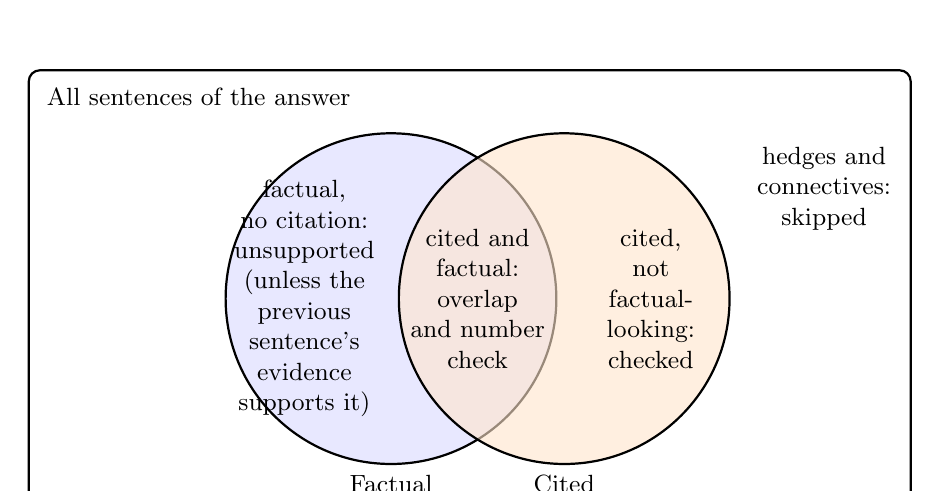
\begin{tikzpicture}[thick]
\draw[rounded corners] (-4.6,-2.6) rectangle (6.6,2.9);
\node[font=\small, anchor=north west] at (-4.5,2.8) {All sentences of the answer};
\draw[fill=blue!15, fill opacity=0.6] (0,0) circle (2.1);
\draw[fill=orange!20, fill opacity=0.6] (2.2,0) circle (2.1);
\node[font=\small, align=center] at (-1.1,0) {factual,\\no citation:\\unsupported\\(unless the\\previous\\sentence's\\evidence\\supports it)};
\node[font=\small, align=center] at (1.1,0) {cited and\\factual:\\overlap\\and number\\check};
\node[font=\small, align=center] at (3.3,0) {cited,\\not\\factual-\\looking:\\checked};
\node[font=\small] at (0,-2.35) {Factual};
\node[font=\small] at (2.2,-2.35) {Cited};
\node[font=\small, align=center] at (5.5,1.4) {hedges and\\connectives:\\skipped};
\end{tikzpicture}
\caption{Venn diagram of answer sentences and their verification}
\label{fig:venn}
\end{figure}

\item Use of above to draw functional dependency graphs and relevant Software modeling methods, techniques
including UML diagrams or other necessities using appropriate tools.

The UML diagrams are given in the SRS and design chapters (use case, activity, state, class and sequence diagrams). Figure~\ref{fig:fdg} is the functional dependency graph of the main functions.

\begin{figure}[!htbp]
\centering
\resizebox{\textwidth}{!}{%
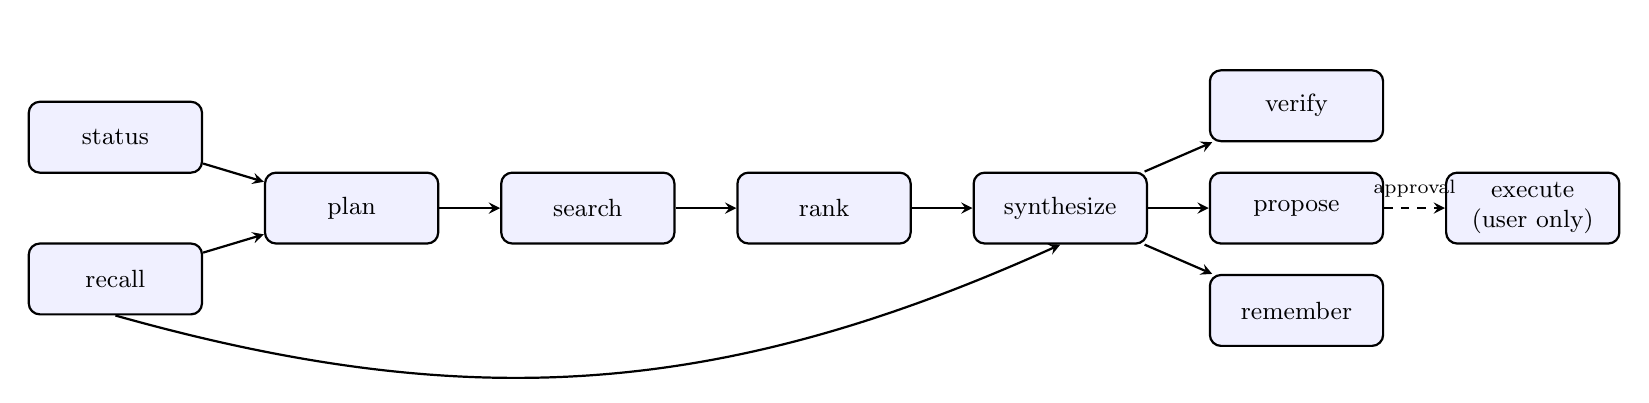
\begin{tikzpicture}[>=stealth, thick,
  fn/.style={draw, rounded corners, minimum width=2.2cm, minimum height=0.9cm, align=center, font=\small, fill=blue!6}]
\node[fn] (st) at (0,0) {status};
\node[fn] (rc) at (0,-1.8) {recall};
\node[fn] (pl) at (3,-0.9) {plan};
\node[fn] (se) at (6,-0.9) {search};
\node[fn] (rk) at (9,-0.9) {rank};
\node[fn] (sy) at (12,-0.9) {synthesize};
\node[fn] (ve) at (15,0.4) {verify};
\node[fn] (pr) at (15,-0.9) {propose};
\node[fn] (re) at (15,-2.2) {remember};
\node[fn] (ex) at (18,-0.9) {execute\\(user only)};
\draw[->] (st) -- (pl);
\draw[->] (rc) -- (pl);
\draw[->] (rc.south) to[bend right=20] (sy.south);
\draw[->] (pl) -- (se);
\draw[->] (se) -- (rk);
\draw[->] (rk) -- (sy);
\draw[->] (sy) -- (ve);
\draw[->] (sy) -- (pr);
\draw[->] (sy) -- (re);
\draw[->, dashed] (pr) -- node[above, font=\scriptsize] {approval} (ex);
\end{tikzpicture}}
\caption{Functional dependency graph}
\label{fig:fdg}
\end{figure}

\item Testing of project problem statement using generated test data (using mathematical models, GUI, Function testing principles, if any) selection and appropriate use of testing tools, testing of UML diagram's reliability. Write also test cases [Black box testing] for each identified functions.
You can use Mathematica or equivalent open source tool for generating test data.

Test data are generated by the sample workspace, whose dates are computed relative to the current day so that time-window questions always have data, and which contains deliberate cross-source conflicts; and by stub model providers and stub connectors in the automated tests. The tool used is Vitest. Black-box test cases for the identified functions are given in Table~\ref{tab:blackbox}; their results are covered by the tests in Chapter~\ref{ch:testing}.

\begin{table}[!htbp]
\begin{center}
\def\arraystretch{1.25}
\small
\begin{tabularx}{\textwidth}{| p{2.3cm} | X | X |}
\hline
Function & Input & Expected output \\ \hline
plan (Fast) & ``what changed this week'' & One sub-question over all sources, window ``last 7 days'' \\ \hline
search & Source down (connection refused) & Failure with name, reason ``could not be reached'', impact; run continues \\ \hline
rank & Duplicate items from two sub-questions & One copy kept; at most 16 (Deep) or 8 (Fast) items \\ \hline
synthesize & No evidence & ``Not found'' text, no model call \\ \hline
verify & ``11 of 19 issues closed [2]'' vs evidence ``11 of 19'' & supported \\ \hline
verify & ``15 of 19 issues closed [2]'' vs evidence ``11 of 19'' & partial (number mismatch) \\ \hline
verify & Factual sentence without citation & unsupported \\ \hline
propose & send\_email without subject & Rejected: ``missing subject'' \\ \hline
execute & Approve by another user & Refused \\ \hline
execute & Second approve & Refused: ``already executed'' \\ \hline
remember & ``Remember that X'' & Memory X stored with salience 0.95 \\ \hline
\end{tabularx}
\end{center}
\caption{Black-box test cases for the identified functions}
\label{tab:blackbox}
\end{table}

\item Additional assignments by the guide. If project type as Entreprenaur, Refer \cite{ehr},\cite{mckinsey},\cite{mckinseyweb}, \cite{govwebsite}

This is an internal project, so the entrepreneurship assignments do not apply. The references are kept for completeness; the McKinsey reports are also used in the motivation. [Additional assignments by the guide, if any, to be added by the team.]
\end{itemize}


\chapter{Project Planner}
\label{app:plan}
The project schedule is planned with a Gantt chart (Figure~\ref{fig:gantt}) for the academic year 2026-2027. Bars show planned durations; the status column shows the state at the time of writing.

\begin{figure}[!htbp]
\centering
\resizebox{\textwidth}{!}{%
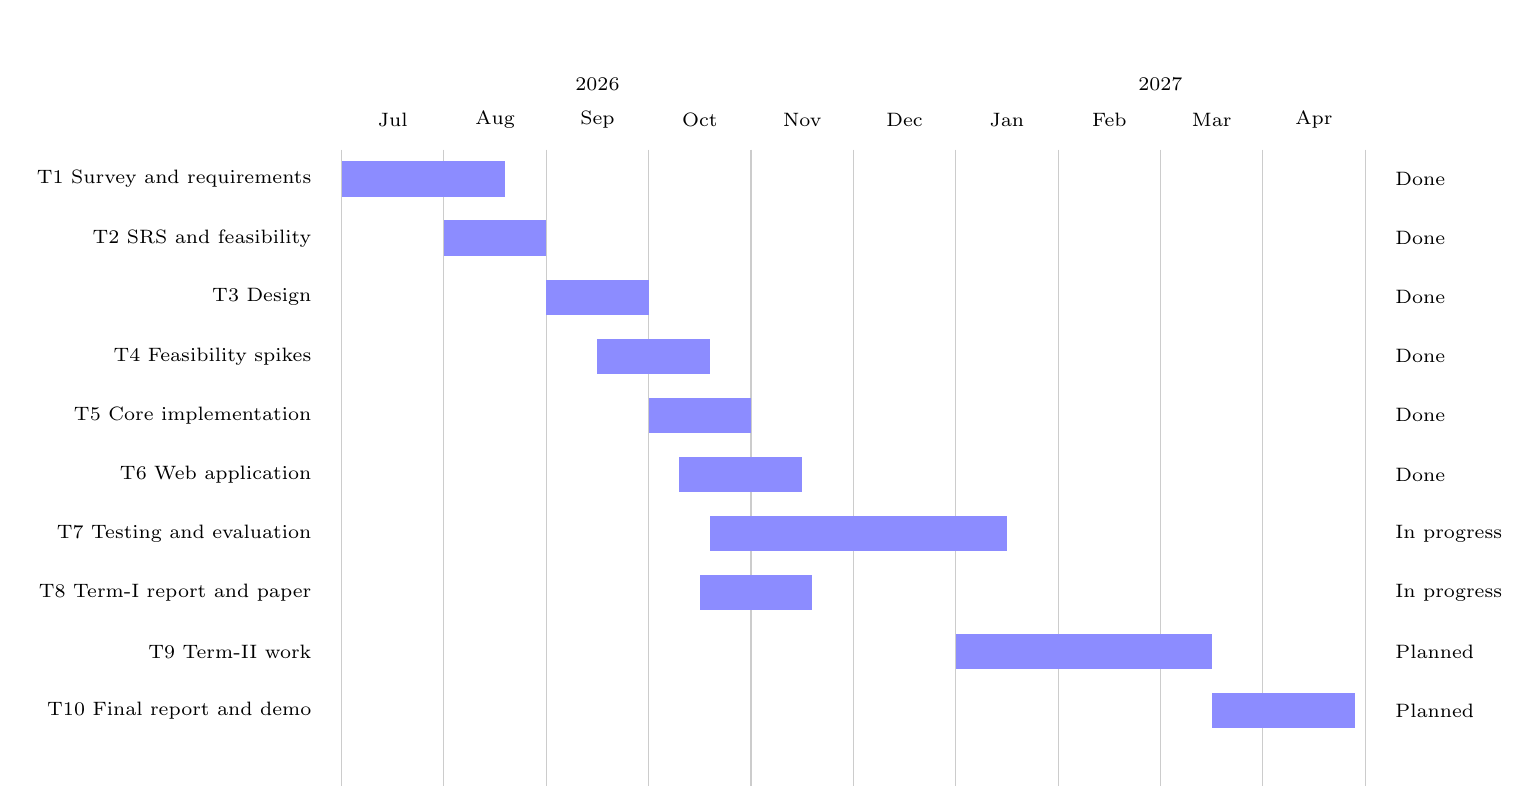
\begin{tikzpicture}[x=1.3cm, y=0.75cm]
\foreach \mo/\lbl in {0/Jul, 1/Aug, 2/Sep, 3/Oct, 4/Nov, 5/Dec, 6/Jan, 7/Feb, 8/Mar, 9/Apr}
{
  \draw[gray!40] (\mo,0.5) -- (\mo,-10.5);
  \node[font=\scriptsize] at (\mo+0.5,1) {\lbl};
}
\draw[gray!40] (10,0.5) -- (10,-10.5);
\node[font=\scriptsize] at (2.5,1.6) {2026};
\node[font=\scriptsize] at (8,1.6) {2027};
\foreach \row/\ts/\te/\tname/\tstat in {
  0/0/1.6/{T1 Survey and requirements}/Done,
  1/1/2/{T2 SRS and feasibility}/Done,
  2/2/3/{T3 Design}/Done,
  3/2.5/3.6/{T4 Feasibility spikes}/Done,
  4/3/4/{T5 Core implementation}/Done,
  5/3.3/4.5/{T6 Web application}/Done,
  6/3.6/6.5/{T7 Testing and evaluation}/{In progress},
  7/3.5/4.6/{T8 Term-I report and paper}/{In progress},
  8/6/8.5/{T9 Term-II work}/Planned,
  9/8.5/9.9/{T10 Final report and demo}/Planned}
{
  \node[font=\scriptsize, anchor=east] at (-0.2,-\row) {\tname};
  \fill[blue!45] (\ts,-\row-0.3) rectangle (\te,-\row+0.3);
  \node[font=\scriptsize, anchor=west] at (10.2,-\row) {\tstat};
}
\end{tikzpicture}}
\caption{Timeline chart (Gantt chart) of the project}
\label{fig:gantt}
\end{figure}

\begin{table}[!htbp]
\begin{center}
\def\arraystretch{1.25}
\small
\begin{tabularx}{\textwidth}{| c | X | c | c | c |}
\hline
Task & Description & Planned start & Planned end & Depends on \\ \hline
T1 & Survey and requirements & Jul 2026 & Aug 2026 & -- \\ \hline
T2 & SRS and feasibility & Aug 2026 & Aug 2026 & T1 \\ \hline
T3 & Design & Sep 2026 & Sep 2026 & T2 \\ \hline
T4 & Feasibility spikes & Sep 2026 & Oct 2026 & T2 \\ \hline
T5 & Core implementation & Oct 2026 & Oct 2026 & T3, T4 \\ \hline
T6 & Web application & Oct 2026 & Nov 2026 & T5 \\ \hline
T7 & Testing and evaluation & Oct 2026 & Jan 2027 & T6 \\ \hline
T8 & Term-I report and paper & Oct 2026 & Nov 2026 & T3 \\ \hline
T9 & Term-II work & Jan 2027 & Mar 2027 & T7, T8 \\ \hline
T10 & Final report and demo & Mar 2027 & Apr 2027 & T9 \\ \hline
\end{tabularx}
\end{center}
\caption{Project planner}
\label{tab:planner}
\end{table}




\chapter{Reviewers Comments of Paper Submitted}
(At-least one technical paper must be submitted in Term-I on the project design in the
conferences/workshops in IITs, Central Universities or UoP Conferences or equivalent International Conferences Sponsored by IEEE/ACM)
\begin{enumerate}
\item Paper Title: Agentic Retrieval-Augmented Generation over Live Workspace Data: A Survey and the Cortex Assistant (draft prepared in IEEE conference format; submission details to be filled by the team)
\item Name of the Conference/Journal where paper submitted : [to be filled by the team]
\item Paper accepted/rejected : [to be filled by the team]
\item Review comments by reviewer : [to be filled by the team]
\item Corrective actions if any : [to be filled by the team]

\end{enumerate}

\chapter{Plagiarism Report}
Plagiarism report: [to be attached by the team after the plagiarism check of the final report].
\chapter{ Term-II Project Laboratory Assignments}
\begin{enumerate}
\item Review of design and necessary corrective actions taking into consideration the feedback report of Term I assessment, and other competitions/conferences participated like IIT, Central Universities, University Conferences or equivalent centers of excellence etc.\\
\emph{Status:} to be completed after the Term-I assessment. [Feedback and corrective actions to be added by the team.]
\item Project workstation selection, installations along with setup and installation report preparations.\\
\emph{Status:} done for development workstations; the setup is described in Chapter~\ref{ch:deploy} and the hardware and software in Tables~\ref{tab:hreq} and~\ref{tab:tools}.
\item Programming of the project functions, interfaces and GUI (if any) as per 1 st Term term-work submission using corrective actions recommended in Term-I assessment of Term-work.\\
\emph{Status:} the functions, interfaces and GUI described in this report are implemented; Term-I corrective actions to be applied after the assessment.
\item Test tool selection and testing of various test cases for the project performed and generate various testing result charts, graphs etc. including reliability testing.\\
\emph{Status:} Vitest and the evaluation harness are in use (Chapter~\ref{ch:testing}, Figures~\ref{fig:chart-g} and~\ref{fig:chart-t}); a larger evaluation with repeated runs is planned.
\textbf{Additional assignments for the Entrepreneurship Project:}
\item Installations and Reliability Testing Reports at the client end.\\
\emph{Status:} not applicable (internal project).

\end{enumerate}
\chapter{Information of Project Group Members}
one page for each student .
\newpage
\begin{enumerate}
\item Name : Ajit Paraskar \hspace{60 mm}\fbox{\parbox[c][75pt][c]{60pt}{\centering\scriptsize [Photo]}}
\item Date of Birth : [to be filled]
\item Gender : [to be filled]
\item Permanent Address : [to be filled]
\item E-Mail : [to be filled]
\item Mobile/Contact No. : [to be filled]
\item Placement Details : [to be filled]
\item Paper Published : [to be filled]

\end{enumerate}
\newpage
\begin{enumerate}
\item Name : Harshvardhan Patil \hspace{52 mm}\fbox{\parbox[c][75pt][c]{60pt}{\centering\scriptsize [Photo]}}
\item Date of Birth : [to be filled]
\item Gender : [to be filled]
\item Permanent Address : [to be filled]
\item E-Mail : [to be filled]
\item Mobile/Contact No. : [to be filled]
\item Placement Details : [to be filled]
\item Paper Published : [to be filled]

\end{enumerate}
\newpage
\begin{enumerate}
\item Name : Prathamesh Kumbhar \hspace{50 mm}\fbox{\parbox[c][75pt][c]{60pt}{\centering\scriptsize [Photo]}}
\item Date of Birth : [to be filled]
\item Gender : [to be filled]
\item Permanent Address : [to be filled]
\item E-Mail : [to be filled]
\item Mobile/Contact No. : [to be filled]
\item Placement Details : [to be filled]
\item Paper Published : [to be filled]

\end{enumerate}
\newpage
\begin{enumerate}
\item Name : Bikram Ghosh \hspace{62 mm}\fbox{\parbox[c][75pt][c]{60pt}{\centering\scriptsize [Photo]}}
\item Date of Birth : [to be filled]
\item Gender : [to be filled]
\item Permanent Address : [to be filled]
\item E-Mail : [to be filled]
\item Mobile/Contact No. : [to be filled]
\item Placement Details : [to be filled]
\item Paper Published : [to be filled]

\end{enumerate}
\end{appendices}


\end{document}
